 %_____________________________________________________________________________
%=============================================================================
% main.tex v6 (10-11-2013) \ldots dibuat oleh Lionov - Informatika FTIS UNPAR
% 
% Ini adalah file utama (main.tex), berisi perintah-perintah yang khusus 
% dibuat untuk template ini
%
% 			JANGAN MENGUBAH APAPUN DI DALAM FILE INI,
%			KECUALI ANDA TAHU APA YANG ANDA LAKUKAN !!!
%
% Jika ada tambahan perintah, dapat anda tuliskan di tempat yang telah disediakan 
% di baris 295 pada file ini
% Jika daftar tabel tidak digunakan, anda harus menghapus (beri komentar) secara
% manual di baris 470
%
% Bug, kritik, saran: silahkan kirimkan via email ke lionov@unpar.ac.id
%
% Perubahan pada versi 6 (10-11-2013):
%	- perbaikan pada abstract dengan paragraf lebih dari satu: perbaikan vertical spacing
%	- perbaikan pada tampilan bab dan lampiran: tidak perlu menuliskan apapun untuk 
%	  menampilkan semuanya (di data.tex) atau -1 jika tidak ada lampiran
%	- halaman bernomor genap untuk halaman romawi sudah dimunculkan
%	- Kurikulum 2013 : perubahan nama buku skripsi 
%
% Perubahan dari versi sebelumnya :
%	versi 5 (21-10-2012)
%	- halaman terakhir setiap bab tidak ada headernya jika kosong
%	versi 4 (06-08-2012)
% 	- penggabungan main.tex, depan.tex dan setup.tex menjadi main.tex
% 	- menambahkan keterangan di lampiran untuk kode program 
% 	- ukuran font dapat diubah langsung di tiap lampiran
% 	versi 3 (09-07-2012): 
%	- Tidak ada di file ini
% 	versi 2 :
% 	- "Daftar Referensi" tidak perlu diubah secara manual (tidak perlu mengubah file bahasai.ldf)
% 	- Bahasa Indonesia dari abstract adalah abstrak (secara otomatis), bukan ringkasan
% 	- Spasi pada buku dokumen final adalah onehalfspacing
%
% to do : - hilangkan secara otomatis daftar tabel/gambar jika tidak digunakan
%         - (IT) aturan penulisan algoritma untuk IT (pakai algo.sty ?)
%=============================================================================

%=============================================================================
% setup.tex v2 (08-07-2012)
% Perubahan pada versi 2:
% - Menambahkan perintah untuk judulINA dan judulENG
% - Menghapus \usepackage{microtype}, yang pada beberapa kasus menjadi masalah
%=============================================================================
% depan.tex v2 (09-07-2012)
% Perubahan pada versi 2:
% - Menambahkan halaman depan dalam bahasa inggris
%=============================================================================

%setup.tex
\documentclass[11pt,a4paper,twoside,openright,notitlepage]{report} 

\usepackage[bahasa]{babel} %bahasa indonesia
\usepackage[T1]{fontenc}  %encoding
% \usepackage{mathptmx}
% \usepackage{venturisold}
% \usepackage{helvet}
% \usepackage{fouriernc} 
\usepackage{abstract} %manipulasi abstract
\usepackage{chappg} % format daftar isi 
\usepackage{color} %warna
\usepackage{etoolbox} %untuk programming if-then
\usepackage{fancyhdr} %format header & footer
\usepackage{float} %penempatan gambar di tempat yg seharusnya
\usepackage[inner=2.5cm,outer=2cm,top=2.5cm,bottom=2.5cm]{geometry} %margin
\usepackage{graphicx} %gambar
\usepackage{listings} %source code
\usepackage{lscape} %landscape untuk source code
\usepackage{multicol} %multiple column
\usepackage{ifthen} % if then
\usepackage[pagewise]{lineno} %line numbering
\usepackage{lipsum} % untuk testing
\usepackage{titlesec} %judul header
\usepackage{tocbibind} %daftar isi, gambar, tabel dll
\usepackage{tocloft} % format daftar isi 
\usepackage{setspace} %line spacing
\usepackage{xstring} %manipulasi string
\usepackage[plainpages=false,pdfpagelabels,unicode]{hyperref} %\autoref, \phantomsection & link 

\usepackage{emptypage}

\let\abstractname\Abstrak

\titleformat{\chapter}[display] {\Large\bfseries\centering}{\MakeUppercase{\chaptertitlename} \thechapter}{15pt}{\Large\MakeUppercase}

\renewcommand{\cftchapfont}{\scshape \bfseries}

\renewcommand{\cfttoctitlefont}{\hfil\Large\bfseries\MakeUppercase}
\renewcommand{\cftaftertoctitle}{\hfill}
\renewcommand{\cftloftitlefont}{\hfill\Large\bfseries\MakeUppercase}
\renewcommand{\cftafterloftitle}{\hfill}
\renewcommand{\cftlottitlefont}{\hfill\Large\bfseries\MakeUppercase}
\renewcommand{\cftafterlottitle}{\hfill}

% Tidak perlu ada kata "Bab", "Gambar" atau "Tabel" di daftar 
% \renewcommand{\cftchappresnum}{{\bf \scshape Bab} } 
% \renewcommand{\cftchapnumwidth}{1.5cm}
% \renewcommand{\cftfigpresnum}{{Gambar\ }} 
% \renewcommand{\cftfignumwidth}{2.5cm}
% \renewcommand{\cfttabpresnum}{{Tabel\ }} 
% \renewcommand{\cfttabnumwidth}{2cm}

\newcommand{\apptoc}{
	% Hapus kata "Lampiran" dari daftar isi
	%\addtocontents{toc}{\protect\renewcommand{\protect\cftchappresnum}{\bf \scshape Lampiran\  }}%
	%\addtocontents{toc}{\protect\renewcommand{\protect\cftchapnumwidth}{2.75cm}}
	\addtocontents{toc}{\protect\renewcommand{\protect\cftchappresnum}{\bf \scshape}}%	

}

\newcommand{\vnama}{Jane Doe}
\newcommand{\vlnama}{John Doe}
\newcommand{\vnpm}{1992700001}
\newcommand{\vprodiINA}{SAINS}
\newcommand{\vprodiENG}{SCIENCE}
\newcommand{\vstaINA}{UJIAN}
\newcommand{\vstaENG}{EXAM}
%\newcommand{\vjudul}{Judul Skripsi/Tugas Akhir}
\newcommand{\vpembu}{Plato}
\newcommand{\vpembs}{Euclid}
\newcommand{\vpengi}{Plato}
\newcommand{\vpengii}{Euclid}
\newcommand{\vtanggal}{1}
\newcommand{\vbulan}{Januari}
\newcommand{\vtahun}{1970}
\newcommand{\vmode}{final}
\newcommand{\vspacing}{double}
\newcommand{\vlineno}{yes}
\newcommand{\vkunciina}{Skripsi, Tugas Akhir}
\newcommand{\vkuncieng}{Undergraduate Thesis, Final Project}
\newcommand{\vkajur}{Jack Doe}
\newcommand{\vkajurmat}{Jack Doe}
\newcommand{\vkajurfis}{Jack Doe}
\newcommand{\vkajurtif}{Jack Doe}

\newcommand{\namanpm}[2]{
	\renewcommand{\vnama}{\uppercase{#1}} \renewcommand{\vlnama}{#1} \hypersetup{pdfauthor={#2 - #1}}
	\renewcommand{\vnpm}{#2} \hypersetup{pdfcreator={#2}} \StrChar{\vnpm}{6}[\vprodiN]
	\ifdefstring{\vprodiN}{1}{
		\renewcommand{\vprodiINA}{MATEMATIKA} \renewcommand{\vprodiENG}{MATHEMATICS} 
		\renewcommand{\vstaINA}{SKRIPSI} \renewcommand{\vstaENG}{FINAL PROJECT} \renewcommand{\vkajur}{\vkajurmat}}{}
	\ifdefstring{\vprodiN}{2}{
		\renewcommand{\vprodiINA}{FISIKA} \renewcommand{\vprodiENG}{PHYSICS} 
		\renewcommand{\vstaINA}{TUGAS AKHIR} \renewcommand{\vstaENG}{FINAL PROJECT} \renewcommand{\vkajur}{\vkajurfis}}{}
	\ifdefstring{\vprodiN}{3}{
		\renewcommand{\vprodiINA}{TEKNIK INFORMATIKA} \renewcommand{\vprodiENG}{INFORMATICS} 
		\renewcommand{\vstaINA}{SKRIPSI} \renewcommand{\vstaENG}{UNDERGRADUATE THESIS} \renewcommand{\vkajur}{\vkajurtif}}{}}

%\newcommand{\judul}[1]{\renewcommand{\vjudul}{\uppercase{#1}}\hypersetup{pdftitle={#1}, pdfsubject={#1}}}
\newcommand{\pembimbing}[2]{\renewcommand{\vpembu}{#1}\renewcommand{\vpembs}{#2}}
\newcommand{\penguji}[2]{\renewcommand{\vpengi}{#1}\renewcommand{\vpengii}{#2}}
\newcommand{\kajur}[3]{\renewcommand{\vkajurmat}{#1}\renewcommand{\vkajurfis}{#2}\renewcommand{\vkajurtif}{#3}}
\newcommand{\tanggal}[3]{\renewcommand{\vtanggal}{#1}\renewcommand{\vtahun}{#3}
	\newcommand{\vcbulan}{#2}
	\ifdefstring{\vcbulan}{1}{\renewcommand{\vbulan}{Januari}}{}
	\ifdefstring{\vcbulan}{2}{\renewcommand{\vbulan}{Februari}}{}
	\ifdefstring{\vcbulan}{3}{\renewcommand{\vbulan}{Maret}}{}
	\ifdefstring{\vcbulan}{4}{\renewcommand{\vbulan}{April}}{}
	\ifdefstring{\vcbulan}{5}{\renewcommand{\vbulan}{Mei}}{}
	\ifdefstring{\vcbulan}{6}{\renewcommand{\vbulan}{Juni}}{}
	\ifdefstring{\vcbulan}{7}{\renewcommand{\vbulan}{Juli}}{}
	\ifdefstring{\vcbulan}{8}{\renewcommand{\vbulan}{Agustus}}{}
	\ifdefstring{\vcbulan}{9}{\renewcommand{\vbulan}{September}}{}
	\ifdefstring{\vcbulan}{10}{\renewcommand{\vbulan}{Oktober}}{}
	\ifdefstring{\vcbulan}{11}{\renewcommand{\vbulan}{November}}{}
	\ifdefstring{\vcbulan}{12}{\renewcommand{\vbulan}{Desember}}{}	
}

\newcommand{\judulINA}[1]{\newcommand{\vjudulINA}{\uppercase{#1}}\hypersetup{pdftitle={#1},pdfsubject={#1}}}
\newcommand{\judulENG}[1]{\newcommand{\vjudulENG}{\uppercase{#1}}\hypersetup{pdftitle={#1},pdfsubject={#1}}}
\newcommand{\abstrakINA}[1]{\newcommand{\vabstrakina}{#1}}
\newcommand{\abstrakENG}[1]{\newcommand{\vabstrakeng}{#1}}
\newcommand{\kunciINA}[1]{\renewcommand{\vkunciina}{#1} \hypersetup{pdfkeywords={#1}}}
\newcommand{\kunciENG}[1]{\renewcommand{\vkuncieng}{#1}}
\newcommand{\untuk}[1]{\newcommand{\vuntuk}{#1}}
\newcommand{\prakata}[1]{\newcommand{\vprakata}{#1}}
\newcommand{\mode}[1]{\renewcommand{\vmode}{#1}}
\newcommand{\linespacing}[1]{\renewcommand{\vspacing}{#1}}
\newcommand{\linenumber}[1]{\renewcommand{\vlineno}{#1}}

\newcommand{\bab}[1]{\newcommand{\vbab}{#1}}
\newcommand{\lampiran}[1]{\renewcommand{\vlmp}{#1}}

\newcommand{\vpilbab}{0}
\newcommand{\vbaba}{0}\newcommand{\vbabb}{0}\newcommand{\vbabc}{0}
\newcommand{\vbabd}{0}\newcommand{\vbabe}{0}\newcommand{\vbabf}{0}
\newcommand{\vbabg}{0}\newcommand{\vbabh}{0}\newcommand{\vbabi}{0}
\newcommand{\vpillmp}{0}
\newcommand{\vlmpa}{0}\newcommand{\vlmpb}{0}\newcommand{\vlmpc}{0}
\newcommand{\vlmpd}{0}\newcommand{\vlmpe}{0}\newcommand{\vlmpf}{0}
\newcommand{\vlmpg}{0}\newcommand{\vlmph}{0}\newcommand{\vlmpi}{0}
\newcommand{\vlmp}{x}

%	\ifdefempty{#1}{\bab{1,2,3,4,5,6,7,8,9} \tampilbab{\vbab}}{
\newcommand{\tampilbab}[1]{
	\ifdefempty{#1}{
		\renewcommand{\vbaba}{1}\renewcommand{\vbabb}{1}\renewcommand{\vbabc}{1}
		\renewcommand{\vbabd}{1}\renewcommand{\vbabe}{1}\renewcommand{\vbabf}{1}
		\renewcommand{\vbabg}{1}\renewcommand{\vbabh}{1}\renewcommand{\vbabi}{1}}{
	\renewcommand{\do}[1]{
		\renewcommand{\vpilbab}{##1}
		\ifdefstring{\vpilbab}{1}{\renewcommand{\vbaba}{1}}{}
		\ifdefstring{\vpilbab}{2}{\renewcommand{\vbabb}{1}}{}
		\ifdefstring{\vpilbab}{3}{\renewcommand{\vbabc}{1}}{}
		\ifdefstring{\vpilbab}{4}{\renewcommand{\vbabd}{1}}{}
		\ifdefstring{\vpilbab}{5}{\renewcommand{\vbabe}{1}}{}
		\ifdefstring{\vpilbab}{6}{\renewcommand{\vbabf}{1}}{}
		\ifdefstring{\vpilbab}{7}{\renewcommand{\vbabg}{1}}{}
		\ifdefstring{\vpilbab}{8}{\renewcommand{\vbabh}{1}}{}
		\ifdefstring{\vpilbab}{9}{\renewcommand{\vbabi}{1}}{}
	}
	\expandafter\docsvlist\expandafter{#1}
	}
}

\newcommand{\tampillmp}[1]{
	\ifdefempty{#1}{
		\renewcommand{\vlmpa}{1}\renewcommand{\vlmpb}{1}\renewcommand{\vlmpc}{1}
		\renewcommand{\vlmpd}{1}\renewcommand{\vlmpe}{1}\renewcommand{\vlmpf}{1}
		\renewcommand{\vlmpg}{1}\renewcommand{\vlmph}{1}\renewcommand{\vlmpi}{1}}{
	\ifdefstring{#1}{-1}{ }{
		\renewcommand{\do}[1]{ 
			\renewcommand{\vpillmp}{##1}
			\ifdefstring{\vpillmp}{A}{\renewcommand{\vlmpa}{1}}{}
			\ifdefstring{\vpillmp}{B}{\renewcommand{\vlmpb}{1}}{}
			\ifdefstring{\vpillmp}{C}{\renewcommand{\vlmpc}{1}}{}
			\ifdefstring{\vpillmp}{D}{\renewcommand{\vlmpd}{1}}{}
			\ifdefstring{\vpillmp}{E}{\renewcommand{\vlmpe}{1}}{}
			\ifdefstring{\vpillmp}{F}{\renewcommand{\vlmpf}{1}}{}
			\ifdefstring{\vpillmp}{G}{\renewcommand{\vlmpg}{1}}{}
			\ifdefstring{\vpillmp}{H}{\renewcommand{\vlmph}{1}}{}
			\ifdefstring{\vpillmp}{I}{\renewcommand{\vlmpi}{1}}{}}
		}
	\expandafter\docsvlist\expandafter{#1}
	}
}

\newcommand{\appspacing}{
	\ifdefstring{\vspacing}{single}{\singlespacing}{}
	\ifdefstring{\vspacing}{onehalf}{\onehalfspacing}{}
	\ifdefstring{\vspacing}{double}{\doublespacing}{}
	\ifdefstring{\vmode}{final}{\onehalfspacing}{}
}

\newcommand{\appline}{
	\ifdefstring{\vmode}{final}{\renewcommand{\vlineno}{no}}{}
	\ifdefstring{\vlineno}{yes}{\linenumbers \def\linenumberfont{\normalfont\tiny\sffamily}}{}
	\ifdefstring{\vlineno}{no}{\lstset{numbers=left, stepnumber=1, numbersep=5pt}}{}
	
}

\newcommand{\appmargin}{
	\ifdefstring{\vmode}{final}{}{\newgeometry{inner=3cm,outer=2.75cm,top=2cm,bottom=2cm}}
}

\renewcommand{\abstractnamefont}{\bf \MakeUppercase}

\makeatletter
\def\headrule{{%
  \if@fancyplain\let\headrulewidth\plainheadrulewidth\fi
  \hrule\@height\footrulewidth\@width\headwidth\vskip2pt%
  \hrule\@height\headrulewidth\@width\headwidth\vskip-\headrulewidth\vskip-4pt
}}
\def\footrule{}

\def\cleardoublepage{
	\clearpage
	\if@twoside \ifodd\c@page
	\else
		\hbox{}
		\vspace{\fill}
		\thispagestyle{empty}
		\newpage
	\if@twocolumn\hbox{}\newpage\fi\fi\fi}
\makeatother

\renewcommand{\headrulewidth}{1.25pt}
\renewcommand{\footrulewidth}{0.25pt}

\setlength{\headheight}{15pt}
\fancyhead[LE,RO]{\thepage}
\fancyhead[RE]{\small{\textsc{\nouppercase{\leftmark}}}}
\fancyhead[LO]{\small{\textsc{\nouppercase{\rightmark}}}}
\fancyfoot{}

\hypersetup{unicode=true,colorlinks=true,linkcolor=blue,citecolor=green,filecolor=magenta, urlcolor=cyan}

\lstset{basicstyle=\tiny, commentstyle=\color{blue}}
\lstset{frame=leftline, tabsize=4, breaklines=true}

%=============================================================================

%tambahkan perintah yang anda butuhkan di sini :

%=============================================================================
%end setup.tex

%_____________________________________________________________________________
%=============================================================================
% data.tex v8 (02-10-2016) \ldots dibuat oleh Lionov - Informatika FTIS UNPAR
%
% Perubahan pada versi 8 (02-10-2016)
%	- Perubahan keterangan pada spacing: Otomatis spasi 1 untuk buku skripsi 
%	  final dan 1.5 untuk buku sidang
%	- Penggunaan kantlipsum
%_____________________________________________________________________________
%=============================================================================

%=============================================================================
% 								PETUNJUK
%=============================================================================
% Ini adalah file data (data.tex)
% Masukkan ke dalam file ini, data-data yang diperlukan oleh template ini
% Cara memasukkan data dijelaskan di setiap bagian
% Data yang WAJIB dan HARUS diisi dengan baik dan benar adalah SELURUHNYA !!
% Hilangkan tanda << dan >> jika anda menemukannya
%=============================================================================

%_____________________________________________________________________________
%=============================================================================
% 								BAGIAN 0
%=============================================================================
% PERHATIAN!! PERHATIAN!! Bagian ini hanya ada untuk sementara saja
% Jika "DAFTAR ISI" tidak bisa berada di bagian tengah halaman, isi dengan XXX
% jika sudah benar posisinya, biarkan kosong (i.e. \daftarIsiError{ })
%=============================================================================
\daftarIsiError{ }
%=============================================================================

%_____________________________________________________________________________
%=============================================================================
% 								BAGIAN I
%=============================================================================
% Tambahkan package2 lain yang anda butuhkan di sini
%=============================================================================
\usepackage{booktabs} 
\usepackage[table]{xcolor}
\usepackage{longtable}
\usepackage{amssymb}
\usepackage{todo}
\usepackage{verbatim} 		%multilne comment
\usepackage{pgfplots}
%=============================================================================

%_____________________________________________________________________________
%=============================================================================
% 								BAGIAN II
%=============================================================================
% Mode dokumen: menetukan halaman depan dari dokumen, apakah harus mengandung 
% prakata/pernyataan/abstrak dll (termasuk daftar gambar/tabel/isi) ?
% - kosong : tidak ada halaman depan sama sekali (untuk dokumen yang 
%            dipergunakan pada proses bimbingan)
% - cover : cover saja tanpa daftar isi, gambar dan tabel
% - sidang : cover, daftar isi, gambar, tabel 
% - sidang_akhir : mode sidang + abstrak + abstract
% - final : seluruh halaman awal dokumen (untuk cetak final)
% Jika tidak ingin mencetak daftar tabel/gambar (misalkan karena tidak ada 
% isinya), edit manual di baris 439 dan 440 pada file main.tex
%=============================================================================
% \mode{kosong}
% \mode{cover}
% \mode{sidang}
 \mode{sidang_akhir}
% \mode{final} 
%=============================================================================

%_____________________________________________________________________________
%=============================================================================
% 								BAGIAN III
%=============================================================================
% Line numbering: penomoran setiap baris, otomatis di-reset setiap berganti
% halaman
% - yes: setiap baris diberi nomor
% - no : baris tidak diberi nomor, otomatis untuk mode final
%=============================================================================
\linenumber{no}
%=============================================================================

%_____________________________________________________________________________
%=============================================================================
% 								BAGIAN IV
%=============================================================================
% Linespacing: jarak antara baris 
% - single	: wajib (dan otomatis jika ingin mencetak buku skripsi, opsi yang 
%			  disediakan untuk bimbingan, jika pembimbing tidak keberatan 
%			  (untuk menghemat kertas)
% - onehalf	: default dan wajib (dan otomatis) jika ingin mencetak dokumen
%             untuk sidang.
% - double 	: jarak yang lebih lebar lagi, jika pembimbing berniat memberi 
%             catatan yg banyak di antara baris (dianjurkan untuk bimbingan)
%=============================================================================
\linespacing{single}
%\linespacing{onehalf}
%\linespacing{double}
%=============================================================================

%_____________________________________________________________________________
%=============================================================================
% 								BAGIAN V
%=============================================================================
% Tidak semua skripsi memuat gambar dan/atau tabel. Untuk skripsi yang seperti
% itu, tidak diperlukan Daftar Gambar dan Daftar Tabel. Sayangnya hal ini 
% sulit dilakukan secara manual karena membutuhkan kedisiplinan pengguna 
% template.  
% Jika tidak akan menampilkan Daftar Gambar/Tabel, isi dengan NO. Jika ingin
% menampilkan, kosongkan parameter (i.e. \gambar{ }, \tabel{ })
%=============================================================================
\gambar{ }
\tabel{ }
%=============================================================================

%_____________________________________________________________________________
%=============================================================================
% 								BAGIAN VI
%=============================================================================
% Bab yang akan dicetak: isi dengan angka 1,2,3 s.d 9, sehingga bisa digunakan
% untuk mencetak hanya 1 atau beberapa bab saja
% Jika lebih dari 1 bab, pisahkan dengan ',', bab akan dicetak terurut sesuai 
% urutan bab (e.g. \bab{1,2,3}).
% Untuk mencetak seluruh bab, kosongkan parameter (i.e. \bab{ })  
% Catatan: Jika ingin menambahkan bab ke-10 dan seterusnya, harus dilakukan 
% secara manual
%=============================================================================
\bab{ }
%=============================================================================

%_____________________________________________________________________________
%=============================================================================
% 								BAGIAN VII
%=============================================================================
% Lampiran yang akan dicetak: isi dengan huruf A,B,C s.d I, sehingga bisa 
% digunakan untuk mencetak hanya 1 atau beberapa lampiran saja
% Jika lebih dari 1 lampiran, pisahkan dengan ',', lampiran akan dicetak 
% terurut sesuai urutan lampiran (e.g. \bab{A,B,C}).
% Jika tidak ingin mencetak lampiran apapun, isi dengan -1 (i.e. \lampiran{-1})
% Untuk mencetak seluruh mapiran, kosongkan parameter (i.e. \lampiran{ })  
% Catatan: Jika ingin menambahkan lampiran ke-J dan seterusnya, harus 
% dilakukan secara manual
%=============================================================================
\lampiran{ }
%=============================================================================

%_____________________________________________________________________________
%=============================================================================
% 								BAGIAN VIII
%=============================================================================
% Data diri dan skripsi/tugas akhir
% - namanpm: Nama dan NPM anda, penggunaan huruf besar untuk nama harus benar
%			 dan gunakan 10 digit npm UNPAR, PASTIKAN BAHWA BENAR !!!
%			 (e.g. \namanpm{Jane Doe}{1992710001}
% - judul : Dalam bahasa Indonesia, perhatikan penggunaan huruf besar, judul
%			tidak menggunakan huruf besar seluruhnya !!! 
% - tanggal : isi dengan {tangga}{bulan}{tahun} dalam angka numerik, jangan 
%			  menuliskan kata (e.g. AGUSTUS) dalam isian bulan
%			  Tanggal ini adalah tanggal dimana anda akan melaksanakan sidang 
%			  ujian akhir skripsi/tugas akhir
% - pembimbing: isi dengan pembimbing anda, lihat daftar dosen di file dosen.tex
%				jika pembimbing hanya 1, kosongkan parameter kedua 
%				(e.g. \pembimbing{\JND}{  } ) , \JND adalah kode dosen
% - penguji : isi dengan para penguji anda, lihat daftar dosen di file dosen.tex
%				(e.g. \penguji{\JHD}{\JCD} ) , \JND dan \JCD adalah kode dosen
% !!Lihat singkatan pembimbing dan penguji anda di file dosen.tex
%=============================================================================
\namanpm{Ariq Rahmaeri}{2011730066}	%hilangkan tanda << & >>
\tanggal{<<tanggal>>}{<<bulan>>}{2016}			%hilangkan tanda << & >>
\pembimbing{Pascal Alfadian}{<<pembimbing pendamping/2>>} %hilangkan tanda << & >>    
\penguji{<<penguji 1>>}{<<penguji 2>>} 				%hilangkan tanda << & >>
%=============================================================================

%_____________________________________________________________________________
%=============================================================================
% 								BAGIAN IX
%=============================================================================
% Judul dan title : judul bhs indonesia dan inggris
% - judulINA: judul dalam bahasa indonesia
% - judulENG: title in english
% PERHATIAN: - langsung mulai setelah '{' awal, jangan mulai menulis di baris 
%			   bawahnya
%			 - Gunakan \texorpdfstring{\\}{} untuk pindah ke baris baru
%			 - Judul TIDAK ditulis dengan menggunakan huruf besar seluruhnya !!
%			 - Gunakan perintah \texorpdfstring{\\}{} untuk baris baru
%=============================================================================
\judulINA{Konversi Jadwal Mengawas Ujian ke Format ICS dengan Apache POI, iCal4j, dan JavaFX}
\judulENG{Convertion Overseen Exam Schedule to ICS Format with Apache POI, iCal4j, and JavaFX}
%_____________________________________________________________________________
%=============================================================================
% 								BAGIAN X
%=============================================================================
% Abstrak dan abstract : abstrak bhs indonesia dan inggris
% - abstrakINA: abstrak bahasa indonesia
% - abstrakENG: abstract in english
% PERHATIAN: langsung mulai setelah '{' awal, jangan mulai menulis di baris 
%			 bawahnya
%=============================================================================
\abstrakINA{Setiap tahun dosen FMIPA UNPAR menerima \textit{printout} jadwal mengawas ujian yang dibuat dengan excel. Walaupun datanya bersifat dijital, namun lebih baik jika data tersebut dibuat terstruktur sehingga dapat dibaca oleh mesin. Dari permalasahan tersebut maka dalam tugas akhir ini akan dibahas tentang pengembangan suatu program yang dapat membaca data excel tersebut dan merubahnya dalam format calendar dijital atau biasa disebut .ics, dengan format .ics jadwal dapat di integrasikan dengan aplikasi iCalendar. Program ini akan menggunakan tiga \textit{library} yaitu Apache POI, iCal4j, dan JavaFX. Apache ROI bertugas membaca struktur data excel sehingga dapat dibaca oleh program, JavaFX berfungsi sebagai \textit{interface} program, dan Ical4j bertugas mengkonversi data yang telah dibaca program kedalam format iCalendar atau .ics .}
\abstrakENG{Every year lecture of FMIPA UNPAR get printout schedule of invigilation in excel format. Although, the excel data is digital data, but it`s better if the data is structured so can be read by machine. Based of the problem above, then this thesis will be discussing about developing program that can read invigilation schedule in excel format and converting the schedule to digital calendar format or commonly called .ics, with .ics format the schedule can be integrated with iCalendar apps . This software will be build based on three library Apache POI, iCal4j, and JavaFX. Apache POI will be handle reading input data so the data can be imported to software, JavaFX is functionate as interface of the software, and iCal4j handles of converting previously read data to iCalendar format or .ics .} 
%=============================================================================

%_____________________________________________________________________________
%=============================================================================
% 								BAGIAN XI
%=============================================================================
% Kata-kata kunci dan keywords : diletakkan di bawah abstrak (ina dan eng)
% - kunciINA: kata-kata kunci dalam bahasa indonesia
% - kunciENG: keywords in english
%=============================================================================
\kunciINA{Apache POI, iCal4j, JavaFX}
\kunciENG{Apache POI, iCal4j, JavaFX}
%=============================================================================

%_____________________________________________________________________________
%=============================================================================
% 								BAGIAN XII
%=============================================================================
% Persembahan : kepada siapa anda mempersembahkan skripsi ini ...
%=============================================================================
\untuk{Keluarga dan kerabat}
%=============================================================================

%_____________________________________________________________________________
%=============================================================================
% 								BAGIAN XIII
%=============================================================================
% Kata Pengantar: tempat anda menuliskan kata pengantar dan ucapan terima 
% kasih kepada yang telah membantu anda bla bla bla ....  
%=============================================================================
\prakata{\kant[3-4]}
%=============================================================================

%_____________________________________________________________________________
%=============================================================================
% 								BAGIAN XIV
%=============================================================================
% Tambahkan hyphen (pemenggalan kata) yang anda butuhkan di sini 
%=============================================================================
\hyphenation{ma-te-ma-ti-ka}
\hyphenation{fi-si-ka}
\hyphenation{tek-nik}
\hyphenation{in-for-ma-ti-ka}
%=============================================================================

%_____________________________________________________________________________
%=============================================================================
% 								BAGIAN XV
%=============================================================================
% Tambahkan perintah yang anda buat sendiri di sini 
%=============================================================================
\newcommand{\vtemplateauthor}{lionov}
\pgfplotsset{compat=newest}
\usetikzlibrary{patterns}
%=============================================================================

% Copyright \textcopyright [Lionov] [09-10-2016]. All rights reserved
%_____________________________________________________________________________
%=============================================================================
% dosen.tex v4 (01-03-2014) \ldots dibuat oleh Lionov - Informatika FTIS UNPAR
%
% Perubahan pada versi 4 (01-03-2014)
% 	- Perubahan ketua jurusan teknik informatika menjadi TAB
%	- Penambahan dosen jurusan informatika (Lucky)
%
% Perubahan pada versi 3 (10-11-2013)
% 	- Perubahan ketua jurusan teknik informatika menjadi MAR
%	- Penambahan dosen jurusan informatika (Joanna, Wahyu)
%	- Penghapusan dosen informatika (Lucky, Dharu)
%
% Perubahan pada versi sebelumnya
% 	versi 2 (25-02-2013)
% 	- Tambahan catatan untuk mhs T. Inf. terkait dosen yg tidak bisa menjadi pemb.
% 	- Update data gelar untuk Taufik (MAT)
% 	- Penambahan baru (Farica-Fisika, Husnul-T.Informatika)
% 	- Dosen keluar atau tidak menjadi pembimbing lagi (Nisa, Ghifary)
%
% 	versi 1 (21-10-2012)
% 	- Data dosen dipindah dari data.tex agar jika ada perubahan/update data dosen
%     mahasiswa tidak perlu mengubah data.tex
% 	- Beberapa dosen Informatika yang tidak boleh menjadi pembimbing digantikan OSS
% 	- Update data gelar untuk Maria (MAT)
% 	- Penambahan baru (Flaviana-Fisika, Elok-Fisika)
% 	- Dosen keluar atau tidak menjadi pembimbing lagi (Monika, David)
%_____________________________________________________________________________
%=============================================================================
% Data dosen dan kajur FTIS - JANGAN MENGUBAH APAPUN DI BAGIAN INI, KECUALI
% untuk mengubah kajur (jika kajur telah berganti orang) atau menambahkan 
% pembimbing anda yang tidak/belum tercantum pada daftar ini atau 
% memperbaiki penulisan gelar jika penguji anda meminta
% perintah: \kajur{1}{2}{3} 1: Matematika 2: Fisika 3: Teknik Informatika
%_____________________________________________________________________________
%=============================================================================
% CATATAN UNTUK MAHASISWA TEKNIK INFORMATIKA :
% dosen yang ditandai * :
% - jika menjadi penguji, tetap, hapus komentar (tanda % & *) agar dapat digunakan
% - jika menjadi pembimbing, ganti dengan (prioritas):
%   1. OSS
%   2. CEN
%   3. TAB
%   mis : jika OSS menjadi penguji, ganti dengan CEN, dst
%_____________________________________________________________________________

\kajur{\FJP}{\PNG}{\TAB}

%dummy person
\newcommand{\JND}{Jane Doe} 
\newcommand{\JHD}{John Doe}
\newcommand{\JCD}{Jack Doe}

% Dosen-dosen Program Studi Matematika
\newcommand{\JDL}{Dr. J. Dharma Lesmono}
\newcommand{\FAR}{Farah Kristiani, M.Si.}
\newcommand{\ERW}{Erwinna Chendra, M.Si.}
\newcommand{\FJP}{Dr. Ferry Jaya Permana}
\newcommand{\AGS}{Agus Sukmana, M.Sc.}
\newcommand{\WSB}{M. Wono Setya Budhi, Ph.D}
\newcommand{\LIM}{Liem Chin, M.Si.}
\newcommand{\HAR}{Y.E. Hariman Sanoe, M.Si.}
\newcommand{\IWS}{Iwan Sugiarto, M.Si.}
\newcommand{\IVM}{Ivonne Martin, M.Sc.}
\newcommand{\OWN}{Livia Owen, M.Si.}
\newcommand{\BNY}{Benny Yong, M.Si.}
\newcommand{\TFK}{Taufik Limansyah, M.T.}
\newcommand{\MRA}{Maria Anestasia, M.Si.}

% Dosen-dosen Program Studi Fisika
\newcommand{\PCT}{Paulus Cahyono Tjiang, Ph.D.}
\newcommand{\BSB}{Prof. B. Suprapto Brotosiswojo, Ph.D.}
\newcommand{\RUS}{Dr. Aloysius Rusli}
\newcommand{\KMG}{Kian Ming, S.Si.}
\newcommand{\SHS}{Sylvia Hastuti Sutanto, Ph.D.}
\newcommand{\JVS}{Janto Vincent Sulungbudi, S.Si.}
\newcommand{\FLA}{Flaviana, S.Si.}
\newcommand{\PNG}{Philips N. Gunawidjaja, Ph.D.}
\newcommand{\ELK}{Elok Fidiani, M.Sc.}
\newcommand{\FEY}{Farica E. Yosafat, M.T.}

% Dosen-dosen Program Studi Teknik Informatika
\newcommand{\CEN}{Dr. rer. nat. Cecilia Esti Nugraheni}
\newcommand{\VSM}{Dr. Veronica Sri Moertini}
\newcommand{\RDL}{Rosa De Lima, M.T.}
\newcommand{\TAB}{Thomas Anung Basuki, Ph.D.}
\newcommand{\LNV}{Lionov, M.Sc.}
\newcommand{\OSS}{Dr. Oerip S. Santoso}
% * \newcommand{\MAR}{Mariskha Tri Aditia, PDEng}
\newcommand{\LCA}{Luciana Abednego, M.T.}
\newcommand{\ELH}{Elisati Hulu, M.T.}
% * \newcommand{\CAN}{Chandra Wijaya, M.T.}
\newcommand{\GDK}{Gede Karya, M.T.}
\newcommand{\NIS}{Nico Saputro, M.T.}
% * \newcommand{\JNH}{Joanna Helga, M.Sc.}
% * \newcommand{\WHY}{Wahyu Pratomo, M.T.}
% * \newcommand{\VER}{Verliyantina, M.T.} 
% * \newcommand{\PAS}{Pascal Alfadian, M.Com.} 
% * \newcommand{\HUS}{Husnul Hakim, M.T.} 
\newcommand{\LAD}{Lucky Adhie, M.T.}

\begin{document}

\def\bibname{Daftar Referensi}
\def\abstractname{Abstrak}

\pagestyle{empty}

%depan.tex
\ifdefstring{\vmode}{kosong}{}{

\pagenumbering{roman}

%cover INA
\begin{center}
	{\Large\bf \vstaINA \\} 	\vspace{1.5cm}
	{\Large \bf \vjudulINA \\} \vspace{2.5cm}
	
\includegraphics[scale=0.4]{Gambar/logo-unpar}\\ \vspace{1cm}
	{\Large \bf \vnama \\} \vspace{0.5cm}
	{\Large \bf NPM: \vnpm \\}
	\vfill
	\Large{ \textbf { 
		PROGRAM STUDI \vprodiINA \\
		FAKULTAS TEKNOLOGI INFORMASI DAN SAINS\\
		UNIVERSITAS KATOLIK PARAHYANGAN\\
		\vtahun 
	}}
\end{center}
\cleardoublepage

%cover ENG
\begin{center}
	{\Large\bf \vstaENG \\} 	\vspace{1.5cm}
	{\Large \bf \vjudulENG \\} \vspace{2.5cm}
	
\includegraphics[scale=0.4]{Gambar/logo-unpar}\\ \vspace{1cm}
	{\Large \bf \vnama \\} \vspace{0.5cm}
	{\Large \bf NPM: \vnpm \\}
	\vfill
	\Large{ \textbf { 
		DEPARTMENT OF \vprodiENG \\
		FACULTY OF INFORMATION TECHNOLOGY AND SCIENCES\\
		PARAHYANGAN CATHOLIC UNIVERSITY\\
		\vtahun 
	}}
\end{center}
\cleardoublepage


% Lembar pengesahan
\ifdefstring{\vmode}{final}{
\begin{center}
	{\Large\bf LEMBAR PENGESAHAN \\} 	\vspace{1.5cm}
	{\Large \bf \vjudulINA \\} 			\vspace{1cm}
	{\Large \bf \vnama \\}				\vspace{0.5cm}
	{\Large \bf NPM: \vnpm \\}			\vspace{1.5cm}
	\large{ \bfseries{
		\begin{centering} 
			Bandung, \vtanggal\ \vbulan\ \vtahun \\ \vspace{0.25cm} Menyetujui,\\
			\vspace{0.75cm}
			\ifdefempty{\vpembs}
					{\centering Pembimbing Tunggal\\ \vspace{2cm} \vpembu\\}
					{ 	\begin{minipage}[b]{0.46\linewidth}
							\centering Pembimbing Utama \\ \vspace{2.25cm} \vpembu \\
						\end{minipage} \hspace{0.5cm}
						\begin{minipage}[b]{0.46\linewidth}
							\centering Pembimbing Pendamping \\	\vspace{2.25cm} \vpembs \\
						\end{minipage}	
					}
		\end{centering}
		\vspace{1.25cm}
		\begin{centering}	
			\begin{minipage}[b]{0.46\linewidth}
				\centering Ketua Tim Penguji \\ \vspace{2.25cm} \vpengi \\
			\end{minipage} \hspace{0.5cm}
			\begin{minipage}[b]{0.46\linewidth}
				\centering Anggota Tim Penguji \\ \vspace{2.25cm} \vpengii 
			\end{minipage}
		\end{centering}
		\vspace{1.5cm} \\
		\centering Mengetahui,\\ \vspace{0.5cm}	
		Ketua Program Studi \\ \vspace{2.25cm} \vkajur\\
	}}			
\end{center}
\cleardoublepage

% Lembar Pernyataan
\vspace*{4cm}
{\Large\bf \centering PERNYATAAN\\} \vspace{1cm}
\noindent
Dengan ini saya yang bertandatangan di bawah ini menyatakan bahwa \MakeLowercase{\vstaINA} dengan judul:  \vspace{0.5cm}
\begin{center}
	{\large \bf \vjudulINA \\}
\end{center}
\vspace{0.75cm}
adalah benar-benar karya saya sendiri, dan saya tidak melakukan penjiplakan atau pengutipan dengan cara-cara yang tidak sesuai dengan etika keilmuan yang berlaku dalam masyarakat keilmuan.
			
Atas pernyataan ini, saya siap menanggung segala risiko dan sanksi yang dijatuhkan kepada saya, apabila di kemudian hari ditemukan adanya pelanggaran terhadap etika keilmuan dalam karya saya, atau jika ada tuntutan formal atau non-formal dari pihak lain berkaitan dengan keaslian karya saya ini.\\
\vspace{0.25cm}

\begin{flushright}	
	Dinyatakan di Bandung,\\
	Tanggal \vtanggal\ \vbulan\ \vtahun \\ \vspace{0.5cm}
	\begin{tabular}{|p{1.75cm}|}
		\hline
		\\ Meterai \\ \\  
		\hline
	\end{tabular}\\
	\vspace{0.5cm} 
	\vlnama \\
	NPM: \vnpm
\end{flushright}
 \cleardoublepage
}{}

% Abstrak & Abstract
\ifthenelse{{\equal{\vmode}{sidang_akhir}}\or{\equal{\vmode}{final}}}{
\ifdefempty{\vabstrakina}{}
	  { \vspace*{4cm}
		\begin{abstract}
			%\noindent \normalsize{\onehalfspacing{\vabstrakina \vspace*{1cm}\\
			\noindent \normalsize{\vabstrakina \vspace*{1cm}\\
			{\bfseries Kata-kata kunci:\ } \vkunciina}
		\end{abstract}
  		\cleardoublepage
	  }
\ifdefempty{\vabstrakeng}{}
	  { \def\abstractname{Abstract}
		\vspace*{4cm}
		\begin{abstract}
			%\noindent \normalsize{\onehalfspacing{\vabstrakeng \vspace*{1cm}\\
			\noindent \normalsize{\vabstrakeng \vspace*{1cm}\\
			{\bfseries Keywords:\ } \vkuncieng}
		\end{abstract}			
 		\cleardoublepage
	  }
}{}

% Lembar persembahan
\ifdefstring{\vmode}{final}{
\ifdefempty{\vuntuk}{}
	  { \vspace*{5cm}
		\begin{quote}
			\em \raggedleft \Large{\vuntuk} 
		\end{quote}
 		\cleardoublepage
	  }

\pagestyle{plain}
	
% Kata pengantar
\ifdefempty{\vprakata}{}
	  {	\chapter*{Kata Pengantar}
		\label{ch:prakata}
		\addcontentsline{toc}{chapter}{Kata Pengantar}
		\vprakata \vspace{0.25cm}
		\begin{flushright}	
			Bandung,\ \vbulan\ \vtahun \\ \vspace{1cm}
			Penulis \\
		\end{flushright}
		\cleardoublepage		
	  }
}{}

\ifthenelse{{\equal{\vmode}{kosong}}\or{\equal{\vmode}{cover}}}{}
	{ \tableofcontents \newpage 	% Daftar isi
	  \listoffigures \newpage 	% Daftar gambar
	  \listoftables \newpage 		% Daftar tabel
	}
	\cleardoublepage
}  

%end depan.tex
\clearpage
\pagenumbering{arabic}

\appmargin
\appspacing
\appline

\pagestyle{fancy}

\tampilbab{\vbab}
\ifdefstring{\vbaba}{1}{%versi 2 (8-10-2016) 
\chapter{Pendahuluan}
\label{chap:intro}
   
\section{Latar Belakang}
\label{sec:latar_belakang}
\indent Jadwal mengawas ujian di FTIS merupakan hal yang rutin dipublikasikan kepada dosen setiap tengah dan akhir semester. Jadwal mengawas tersebut dipublikasikan oleh tata usaha. Sebelum dibagikan jadwal mengawas dibuat dalam file excel, lalu dicetak dan dibagikan kepada setiap dosen. Format jadwal mengawas ujian bersifat umum, dalam arti jadwal tersebut menyimpan nama semua dosen yang mengawas, nama mata kuliah, dan tempat pelaksanaan ujian. Dosen diharuskan melihat satu persatu baris untuk mendapatkan informasi mengenai waktu, nama matakuliah, dan tanggal dosen tersebut mengawas. Walaupun jadwal mengawas tersebut telah disusun dalam file excel, namun tetap dirasa kurang efisien karena tidak tersusun berdasarkan dosen yang mengawas dan memungkinkan terjadi kesalahan dalam membaca jadwal oleh dosen. 
iCalendar merupakan format file \textit{calendar} pada komputer yang memudahkan penggunanya untuk mengirimkan undangan \textit{meeting} dan melakukan pekerjaan bersama pengguna lainnya, via email, atau file \textit{sharing} menggunakan ekstensi .ics . Format iCalendar sendiri telah didukung dan kompatibel dengan produk lainnya, seperti Google Calendar, Microsoft Outlook, Yahoo Calendar, Mozilla Thunderbird, Apple Calendar.
Dari penjelasan diatas, tugas akhir ini dimaksudkan untuk memudahkan dosen untuk melihat jadwal mengawas ujian dimanapun dan kapanpun. Pengembangan perangkat lunak ini menggunakan tiga library yaitu Apache POI, JavaFX, dan iCal4j.    

\section{Rumusan Masalah}
\label{sec:rumusan}
Berdasarkan penjelasan di latar belakang, maka dapat dipaparkan rumusan masalah sebagai berikut :
\begin{enumerate}
	\item Bagaimana perangkat lunak dapat membaca file excel jadwal mengawas ujian yang dibuat oleh TU ?
	\item Bagaimana menampilkan jadwal ke layar ?
	\item Bagaimana perangkat lunak mengkonversi jadwal mengawas menjadi iCalendar ? 
\end{enumerate}


\section{Tujuan}
\label{sec:tujuan}
Tujuan dari karya ilmiah ini dapat dipaparkan sebagai berikut:
\begin{enumerate}
	\item Merancang PL yang mampu membaca file excel yang dipublikasikan oleh TU.
	\item Membuat PL yang mampu menampilkan jadwal mengawas ujian yang telah dibaca ke layar.
	\item Merancang PL dapat mengkonversi jadwal mengawas menjadi iCalendar.
\end{enumerate}

\section{Batasan Masalah}
\label{sec:batasan}
Batasan masalah dalam penelitian ini agar dapat fokus pada pengembangan perangkat lunak konversi jadwal mengawas ujian :
\begin{itemize}
	\item Diasumsikan TU menggunakan layout yang sama setiap tahunnya.  
\end{itemize}

\section{Metodologi}
\label{sec:metlit}
Untuk menunjang penelitian maka diperlukan data untuk pengujian maupun pengetahuan teori yang akan diterapkan. Berikut adalah kegiatan yang akan dilakukan:
\begin{enumerate}
		\item Melakukan studi pustaka mengenai
			\begin{enumerate}
				\item Apache POI
				\item JavaFX
				\item iCal4j
				\item Memperdalam Netbeans
			\end{enumerate}
		\item Melakukan analisis pada file excel jadwal mengawas ujian yang dikeluarkan oleh TU.
		\item Melakukan perancangan yang terdiri dari use case, diagram aktifitas, dan \textit{user interface}.
		\item Mengimplementasikan rancangan kedalam Netbeans. 
		\item Melakukan pengujian perangkat lunak dengan berbagai kemungkinan kasus.
		\item Menyimpulkan atas serangkaian pengembangan yang dilakukan
		\item Menulis dokumen skripsi
	\end{enumerate}

\section{Sistematika Pembahasan}
\label{sec:sispem}
\begin{enumerate}
	\item Bab 1 Pendahuluan\\
	Bab ini berisi tentang latar belakang, rumusan masalah, tujuan, batasan masalah, metodologi penelitian, dan sistematika pembahasan.
	\item Bab 2 Dasar Teori\\
	Bab ini berisi tentang teori dasar tentang JavaFX, Apache POI, iCal4j.
	\item Bab 3 Analisis\\
	Bab ini berisi tentang analisis kebutuhan dan fitur PL, diagram aktifitas PL, use case, diagram kelas.
	\item Bab 4 Perancangan\\
	Bab ini berisi tentang perancangan kelas dalam PL dan gambaran \textit{user interface}.
	\item Bab 5 Implementasi dan Pengujian\\
	Bab ini berisi tentang penerapan hasil rancangan pada bab sebelumnya serta pengujian perangkat lunak.
	\item Bab 6 Kesimpulan dan Saran\\
	Bab ini berisi tentang kesimpulan yang didapatkan dari hasil pengujian serta saran apabila ingin melanjutkan pengembangan ini.
\end{enumerate}}{}
\ifdefstring{\vbabb}{1}{%versi 2 (8-10-2016)
\chapter{Landasan Teori}
\label{chap:teori}
Pada bab ini akan dijelaskan mengenai konsep-konsep dasar pendukung PL, yaitu JavaFX, Apache POI, iCal4j.

\section{Apache POI}
\label{sec:apache} 

POI merupakan singkatan dari \textit{Poor Obfuscation Implementation} yang dikembangkan oleh Apache. Apache POI pada hakikatnya merupakan \textit{library} untuk memanipulasi dan menciptakan sesuatu melalui Java API( \textit{application programming interface}) dengan memanipulasi berbagai format file berdasarkan \textit{Office Open XML standards}(OOXML) dan dokumen \textit{Microsoft OLE 2 Document Compound Format}(OLE2), Singkatnya dengan library ini memungkinkan untuk membaca dan menulis pada MS Excel menggunakan Java.\cite{apachepoi} \\


\subsection{Komponen Apache POI}
\label{subs:komponen} 
Untuk membaca aplikasi MS Office Apache POI mempunyai modul berisi komponen java api untuk membaca dokumen dengan format OLE2 dan OOXML. Berikut ini komponen-komponen dalam Apache POI.\cite{apachepoi}  

\begin{enumerate}
	\item Excel \textit{workbooks} (HSSF dan XSSF)
	\item Word \textit{document} (HWPF dan XWPF)
	\item PowerPoint \textit{presentation} (HSLF dan XSLF)
	\item Outlook (HSMF)
	\item Visio (HDGF dan XDGF)
	\item Publisher (HPBF)
\end{enumerate}

HSSF merupakan singkatan dari \textit{Horrible Spreadsheet Format}, sedangkan XSSF merupakan singkatan dari \textit{XML Spreadsheet Format}. HSSF dan XSSF memberikan cara untuk membuat, membaca, dan memodifikasi XLS spreadsheet. Pada sub bab ini akan difokuskan untuk membahas XSSF sesuai kebutuhan untuk menganalisa file excel jadwal mengawas ujian yang dikeluarkan oleh TU FTIS.\cite{apachepoi}


\subsection{Kelas Inti Apache POI}
\label{subs:kelas_inti}

\begin{figure}[H]
	\centering
	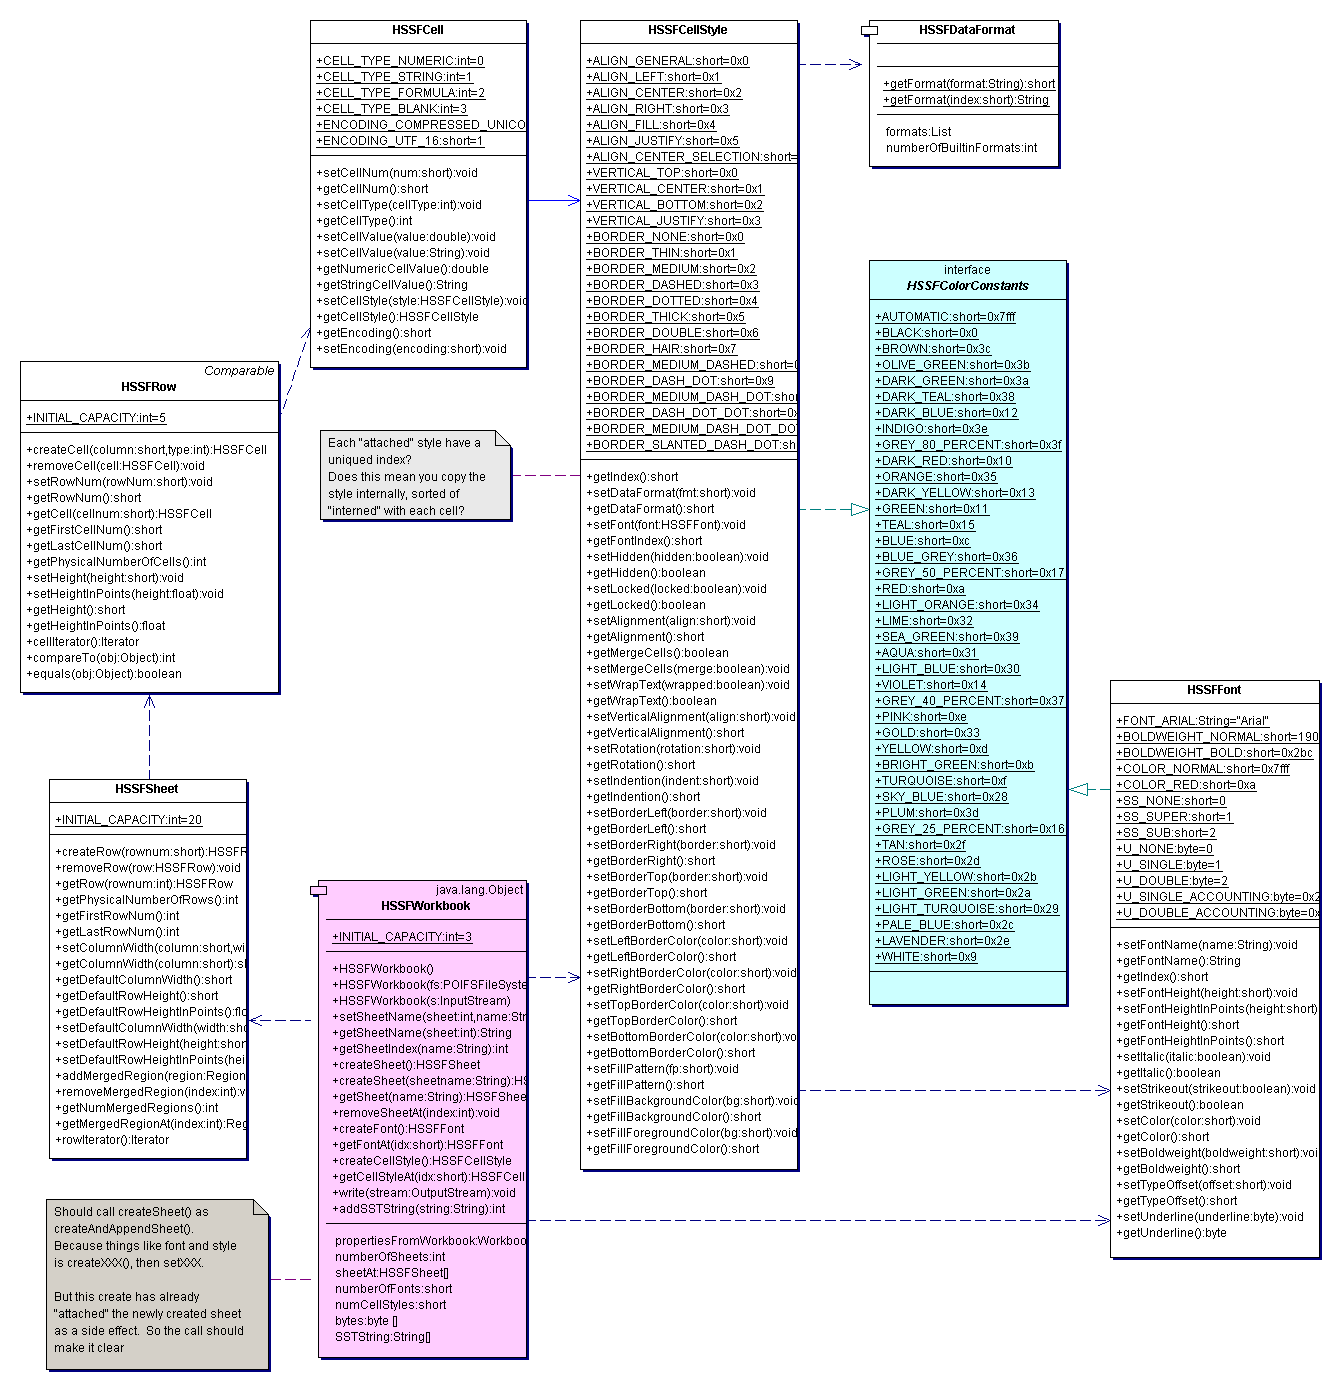
\includegraphics[scale=0.3]{Gambar/hssf}
	\caption{Kelas diagram hssf}
\end{figure}

Pada sub bab ini akan membahas introduksi mengenai beberapa kelas dan method yang ada di Apache POI API yang merupakan bagian penting untuk bekerja dengan file excel mengunakan program Java. Kelas HSSF dan XSSF mempunyai struktur kelas yang sama yang membedakan adalah kompatibilitas versi format excel yang dapat dibaca. \cite{apachepoi2}

\subsubsection{Workbook}
\label{subs:workbook} 
\textbf{org.apache.poi.ss.usermodel} \textit{package} merupakan \textit{super-interface} dari semua kelas yang berhubungan dengan pembuatan atau me-\textit{maintain} Excel workbook. Dua kelas yang mengimplementasikan \textit{interface} tersebut sebagai berikut:\cite{apachepoi2}

\begin{itemize}
	\item \textbf{HSSFWorkbook} : Kelas ini mempunyai method yang dapat membaca dan menulis file Microsoft Excel dengan format .xls. Kelas ini kompatibel dengan MS-Office versi 97-2003.
	\item \textbf{XSSFWorkbook} : Kelas ini mempunyai method untuk menulis dan membaca Microsoft Excel dan OpenOffice xml dengan format .xlsx. Kelas ini kompatibel dengan MS-Office versi 2007 atau versi barunya.
\end{itemize}  

\subsubsection{XSSFWorkbook}
\label{subs:XSSFWorkbook}
Kelas ini merepresentasikan baik \textit{high} dan \textit{low} level format file excel. XSSFWorkbook merupakan kelas yang berada dalam \textit{package} \textbf{org.apache.xssf.usermodel} dan mengimplementasikan antarmuka workbook. Berikut ini list method dan constructor dalam kelas ini.\cite{apachepoi2}
\\
\noindent \textbf{Class Constructor}
\begin{table}[H]
		\centering
		\caption{Tabel kelas Konstruktor XSSFWorkbook}
		\label{tab:konstrukXSSF}
	\begin{tabular}{|c|p{12cm}|}
		\hline
		\textbf{No} & \textbf{Constructor dan Deskripsi} \\ \hline \hline
		1 & \textbf{XSSFWorkbook()}\\
			&	Membuat objek XSSFWorkbook.\\ \hline 
		2 & \textbf{XSSFWorkbook(java.io.File file)}\\
			&	Membangun sebuah objek XSSFWorkbook dari file yang diberikan.\\ \hline
		3 & \textbf{XSSFWorkbook(java.io.InputStream is)}\\
			&	Membangun sebuah object XSSFWorkbook dengan \textit{buffering} semua input stream ke dalam memory, dilanjutkan dengan membuka objek OPCPackage.\\ \hline 
		4 & \textbf{XSSFWorkbook(java.lang.String path)}\\
			&	Membangun sebuah objek XSSFWorkbook dengan diberikan \textit{full path} dari sebuah file.\\ \hline
	\end{tabular}
\end{table}

\noindent \textbf{Class Methods}

\begin{table}[H]
		\centering
		\caption{Tabel kelas method XSSFWorkbook}
		\label{tab:methodXSSF}
	\begin{tabular}{|c|p{12cm}|}
		\hline
		\textbf{No} & \textbf{Method dan Deskripsi} \\ \hline \hline
		1 & \textbf{CreateSheet()}\\
			&	Menciptakan atau menambahkan sebuah XSSFSheet pada workbook.\\ \hline 
		2 & \textbf{createSheet(java.lang.String sheetname)}\\
			&	Membuat sheet baru untuk workbook .\\ \hline
		3 & \textbf{createFont()}\\
			&	Membuat font baru dan menambahkannya pada tabel font pada workbook.\\ \hline 
		4 & \textbf{createCellStyle()}\\
			&	Membuat XSSFCellStyle Baru dan menambahkannya pada tabel style workbook.\\ \hline
		5 & \textbf{setPrintArea(int sheetIndex, int startColumn, int endColumn, int startRow,int endRow)}\\
			&	Menentukan area print dari kertas dengan parameter yang spesifik.\\ \hline	
	\end{tabular}
	\end{table}
	
\subsubsection{Sheet}
\label{subs:Sheet}
\textit{Sheet} merupakan sebuah interface dibawah package org.apache.ss.usermodel. \textit{Sheet} merupakan representasi sebuah \textit{grid} dari cell.\cite{apachepoi2}
	
\subsubsection{XSSFSheet}
\label{subs:XSSFSheet}
Kelas ini merupakan representasi dari \textit{high level} excel spreadsheet. Kelas ini berada di bawah package org.apache.poi.hssf.usermodel.\cite{apachepoi2}
\\
\noindent \textbf{Class Constructor}
\begin{table}[H]
		\centering
		\caption{Tabel kelas Konstruktor XSSFSheet}
		\label{tab:konstrukXSSFSheet}
	\begin{tabular}{|c|p{12cm}|}
		\hline
		\textbf{No} & \textbf{Constructor dan Deskripsi} \\ \hline \hline
		1 & \textbf{XSSFSheet()}\\
			&	Membuat baru XSSFSheet yang disebut XSSFWorkbook dalam pembuatan sheet baru .\\ \hline 
	\end{tabular}
\end{table}

\noindent \textbf{Class Methods}
\begin{table}[H]
		\centering
		\caption{Tabel kelas method XSSFSheet}
		\label{tab:methodXSSFSheet}
	\begin{tabular}{|c|p{12cm}|}
		\hline
		\textbf{No} & \textbf{Constructor dan Deskripsi} \\ \hline \hline
		1 & \textbf{addMergedRegion(CellRangeAddress region))}\\
			&	Menambahkan gabungan wilayah dari cell.(beberapa cell menjadi satu)   .\\ \hline 
		2 & \textbf{autoSizeColumn(int column)}\\
			& Menyesuaikan lebar kolom agar sesuai dengan isinya.\\ \hline
		3 & \textbf{iterator()}\\
			&	Method ini alias rowIterator() untuk memungkinkan foreach loop .\\ \hline
		4 & \textbf{addHyperlink(XSSFHyperlink hyperlink)}\\
			&	Mendaftarkan sebuah hyperlink kedalam koleksi hyperlink yang ada di sheet.\\ \hline	
	\end{tabular}
\end{table}

\subsubsection{Row}
\label{subs:Row}
Row merupakan interface berada di bawah \textit{package} \textbf{org.apache.poi.ss.usermodel}. Row ini digunakan untuk \textit{high-level representation} dari sebuah row pada sebuah spreadsheet. Row juga merupakan super-interface dari semua kelas yang mewakili row dalam POI \textit{Library}.\cite{apachepoi2}

\subsubsection{XSSFRow}
\label{subs:XSSFRow}
XSSFRow merupakan sebuah kelas di bawah \textit{package} \textbf{org.apache.poi.xssf.usermodel} dan mengimplementasi Row interface. Selain itu, kelas ini dapat membuat row dalam sebuah spreadsheet. List dibawah ini merupakan \textit{method} dan constructors pada kelas ini.\cite{apachepoi2}
 \\ 
\noindent \textbf{Class Methods}
\begin{table}[H]
		\centering
		\caption{Tabel kelas method XSSFRow}
		\label{tab:methodXSSFRow}
	\begin{tabular}{|c|p{12cm}|}
		\hline
		\textbf{No} & \textbf{Deskripsi} \\ \hline \hline
		1 & \textbf{createCell(int columnIndex)}\\
			&	Membuat cell baru dalam baris.\\ \hline 
		2 & \textbf{setHeight(short height)}\\
			&	Mengatur tinggi dalam satuan short.\\ \hline
	\end{tabular}
\end{table}

\subsubsection{Cell}
\label{subs:Cell}
Cell merupakan interface yang berada di bawah \textit{package} \textbf{org.apache.poi.ss.usermodel}. Cell merupakan sebuah super-interface dari semua kelas yang mewakili cell dalam baris sebuah spreadsheet.\\

Cell dapat berupa berbagai atribut seperti \textit{blank, numeric, date, error}. Sebelum ditambahkan ke baris cell memiliki nomer tersendiri(dari mulai 0).\cite{apachepoi2}

\subsubsection{XSSFCell}
\label{subs:XSSFCell}  
Kelas ini berada di bawah \textit{package} \textbf{org.apache.poi.xssf.usermodel}. Kelas ini mewakili cell interface. XSSFCell adalah \textit{high-level representation} cell dalam row dari sebuah spreadsheet.\cite{apachepoi2}

\subsubsection{Ringkasan Tipe Cell}
\label{subs:Ringkasan_Tipe_Cell}
List di bawah ini adalah sebagian \textit{field} dari kelas XSSFCell beserta deskripsinya.
\begin{table}[H]
		\centering
		\caption{Tabel ringkasan tipe cell}
		\label{tab:ringkasan_tipe_cell}
	\begin{tabular}{|c|c|}
		\hline
		\textbf{Tipe Cell} & \textbf{Deskripsi} \\ \hline \hline
		CELL\_TYPE\_BLANK & Representasi cell kosong\\ \hline 
		CELL\_TYPE\_BOOLEAN &	Representasi cell Boolean (True atau False)\\ \hline 
		CELL\_TYPE\_ERROR & Representasi nilai error dari cell\\ \hline
		CELL\_TYPE\_FORMULA	&	Representasi dari hasil sebuah formula dalam cell\\ \hline
		CELL\_TYPE\_NUMERIC	&	Representasi dari data numerik dalam cell\\ \hline
		CELL\_TYPE\_STRING	&	Representasi dari String(teks) dalam cell\\ \hline
	\end{tabular}
\end{table}
	
\noindent \textbf{Class Methods}
\begin{table}[H]
		\centering
		\caption{Tabel kelas method XSSFCell}
		\label{tab:methodXSSFCell}
	\begin{tabular}{|c|p{12cm}|}
		\hline
		\textbf{No} & \textbf{Deskripsi} \\ \hline \hline
		1 & \textbf{setCellStyle(CellStyle style)}\\
			&	Mengatur style untuk cell.\\ \hline 
		2 & \textbf{setCellType(int cellType)}\\
			&	Mengatur tipe cell (numeric, formula, atau String).\\ \hline
		3 & \textbf{setCellValue(boolean value)}\\
			&	Mengatur nilai bolean dalam sebuah cell.\\ \hline
		4 & \textbf{setCellValue(java.util.Calendar value)}\\
			&	Mengatur nilai tanggal dari cell .\\ \hline	
		5 & \textbf{setCellValue(double value)}\\
			&	Mengatur nilai numerik dari cell.\\ \hline
		6 & \textbf{setCellValue(java.lang.String str)}\\
			&	Mengatur nilai String dari cell.\\ \hline
		7 & \textbf{setHyperlink(Hyperlink hyperlink)}\\
			&	Menambahkan sebuah hyperlink kedalam cell\\ \hline					
	\end{tabular}
\end{table}

\subsubsection{XSSFCellStyle}
\label{subs:XSSFCellStyle}
XSSFCellStyle merupakan sebuah kelas yang berada di bawah \textit{package} \textbf{org.apache.poi.usermodel}. kelas ini memberikan infomarsi yang mungkin mengenai format konten pada suatu cell dari spreadsheet. Kelas ini juga memberikan opsi untuk merubah format tersebut. Kelas ini mewakili \textit{CellStyle interface}.\cite{apachepoi2}

\subsubsection{Ringkasan Cell Style}
\label{subs:Ringkasan_Cell_Style}
List di bawah ini adalah sebagian \textit{field} yang diwariskan dari CellStyle interface.\cite{apachepoi2}\\

\begin{table}[H]
		\centering
		\caption{Tabel ringkasan cell style}
		\label{tab:ringkasan_cell_style}
		
	
	\begin{tabular}{|c|c|}
		\hline
		\textbf{Nama Field} & \textbf{Deskripsi Field} \\ \hline \hline
		ALIGN\_CENTER & Rata tengah \textit{content cell}\\ \hline 
		ALIGN\_CENTER\_SELECTION &	Posisi seleksi tengah horizontal\\ \hline 
		ALIGN\_FILL & Mencocokan ukuran \textit{cell content} \\ \hline
		ALIGN\_JUSTIFY	&	Mencocokan ukuran \textit{cell content} terhadap lebarnya\\ \hline
		ALIGN\_LEFT	&	Rata kiri \textit{cell content}\\ \hline
		ALIGN\_RIGHT &	Rata kanan \textit{cell content}\\ \hline
		BORDER\_DASH\_DOT &	\textit{Cell style} dengan garis dan titik \\ \hline
		BORDER\_DOTTED &	\textit{Cell style} dengan border titik\\ \hline
		BORDER\_DASHED &	\textit{Cell style} dengan border garis\\ \hline
		BORDER\_THICK &	\textit{Cell style} dengan border tebal\\ \hline
		BORDER\_THIN &	\textit{Cell style} dengan border tipis\\ \hline
		VERTICAL\_BOTTOM &	Posisi \textit{cell content} vertikal kebawah\\ \hline
		VERTICAL\_CENTER & \textit{cell content} vertikal ketengah\\ \hline
		VERTICAL\_JUSTIFY &	Posisi \textit{cell content} sejajar secara vertikal \\ \hline
		VERTICAL\_TOP &	Posisi selaras keatas secara vertikal\\ \hline
	\end{tabular}
\end{table}

\noindent \textbf{Class Constructor}
\begin{table}[H]
		\centering
		\caption{Tabel kelas konstruktor XSSFCellStyle}
		\label{tab:konstrukXSSFCellStyle}
	\begin{tabular}{|c|p{15cm}|}
		\hline
		\textbf{No} & \textbf{Constructor dan Deskripsi} \\ \hline \hline
		1 & \textbf{XSSFCellStyle(int cellXfId, int cellStyleXfId, StylesTable stylesSource, ThemesTable theme)}\\
			&	Menciptakan cell style dengan bagian yang sudah disediakan.\\ \hline
		2 & \textbf{XSSFCellStyle(StylesTable stylesSource)}\\
			&	Membuat cell Style kosong.\\ \hline 	
	\end{tabular}
\end{table}

\noindent \textbf{Class Methods}
\begin{table}[H]
		\centering
		\caption{Tabel kelas method XSSFCellStyle}
		\label{tab:methodXSSFCellStyle}
	\begin{tabular}{|c|p{12cm}|}
		\hline
		\textbf{No} & \textbf{Method dan Deskripsi} \\ \hline \hline
		1 & \textbf{setAlignment(short align)}\\
			&	Mengatur style secara horizontal untuk cell.\\ \hline 
		2 & \textbf{setBorderBottom(short border)}\\ \hline
		3 & \textbf{setBorderColor(XSSFCellBorder.BorderSide side, XSSFColor color)}\\
			&	Mengatur warna untuk border yang dipilih.\\ \hline
		4 & \textbf{setBorderLeft(Short border)}\\
			&	Mengatur tipe border untuk border kiri dari cell .\\ \hline	
		5 & \textbf{setBorderRight(short border)}\\
			&	Mengatur tipe border untuk border kanan dari cell .\\ \hline
		6 & \textbf{setBorderTop(short border)}\\
			&	Mengatur tipe border untuk border atas dari cell \\ \hline
		7 & \textbf{setFillBackgroundColor(XSSFColor color)}\\
			&	Mengatur latar belakang warna yang diwakili oleh nilai XSSFColor\\ \hline
		8 & \textbf{setFillForegroundColor(XSSFColor color)}\\
			&	Mengatur latar depan warna yang diwakili oleh nilai XSSFColor\\ \hline
		9 & \textbf{setFillPattern(short fp)}\\
			&	Menentukan isi informasi cell dengan pola dan warna solid\\ \hline
	  10 & \textbf{setFont(Font font)}\\
			 &	Mengatur font\\ \hline
		11 & \textbf{setRotation(short rotation)}\\
			 &	Mengatur derajat rotasi pada teks dalam cell.\\ \hline
		12 & \textbf{setVerticalAlignment(short align)}\\
			 &	Menetapkan tipe posisi vertical pada cell\\ \hline		
	\end{tabular}
\end{table}


\subsubsection{XSSFColor}
\label{subs:XSSFColor}
XSSFColor merupakan sebuah kelas dibawah \textit{package} \textbf{org.apache.poi.xssf.usermodel}. Kelas ini mewakili warnma pada spreadsheet. Kelas ini mengimplementasika interface warna. List dibawah ini merupakan beberapa method XSSFColor dan constructornya.\cite{apachepoi2}
\\
\noindent \textbf{Class Constructor}
\begin{table}[H]
		\centering
		\caption{Tabel kelas konstruktor XSSFColor}
		\label{tab:KonstrukXSSFColor}
	\begin{tabular}{|c|p{12cm}|}
		\hline
		\textbf{No} & \textbf{Constructor dan Deskripsi} \\ \hline \hline
		1 & \textbf{XSSFColor()}\\
			&	Menciptakan \textit{instance} baru dari XSSFColor.\\ \hline
		2 & \textbf{XSSFColor(byte[] rgb)}\\
			&	Membuat  \textit{instance} baru dari XSSFColor menggunakan RGB.\\ \hline
		3 & \textbf{XSSFColor(java.awt.Color clr))}\\
			&	Membuat  \textit{instance} baru dari XSSFColor menggunakan kelas warna dari \textit{awt package}.\\ \hline 		
	\end{tabular}
\end{table}

\noindent \textbf{Class Methods}
\begin{table}[H]
		\centering
		\caption{Tabel kelas method XSSFColor}
		\label{tab:methodXSSFColor}
	\begin{tabular}{|c|p{12cm}|}
		\hline
		\textbf{No} & \textbf{Method dan Deskripsi} \\ \hline \hline
		1 & \textbf{setAuto(boolean auto)}\\
			&	Mengatur sebuah nilai boolean untuk mengindikasikan bahwa ctColor bersifat otomatis dan bergantung pada sistem ctColor.\\ \hline
		2 & \textbf{setIndexed(int indexed)}\\
			&	Mengatur nilai indeks ctColor sebagai sistem ctColor.\\ \hline
	\end{tabular}
\end{table}

\subsubsection{XSSFFFont}
\label{subs:XSSFFFont}
XSSFFont merupakan kelas dibawah \textit{package} \textbf{org.aoache.poi.xssf.usermodel}. Kelas ini mengimplementasikan \textit{Font interface} dan oleh sebab itu kelas ini dapat menangani font berbeda pada sebuah workbook.\cite{apachepoi2}
\\
\noindent \textbf{Class Constructor}
\begin{table}[H]
		\centering
		\caption{Tabel kelas konstruktor XSSFFont}
		\label{tab:KonstrukXSSFFont}
	\begin{tabular}{|c|p{12cm}|}
		\hline
		\textbf{No} & \textbf{Constructor dan Deskripsi} \\ \hline \hline
		1 & \textbf{XSSFFont()}\\
			&	Menciptakan \textit{instance} baru dari XSSFFont.\\ \hline
	\end{tabular}
\end{table}

\noindent \textbf{Class Methods}
\begin{table}[H]
		\centering
		\caption{Tabel kelas method XSSFFont}
		\label{tab:methodXSSFFont}
	\begin{tabular}{|c|p{12cm}|}
		\hline
		\textbf{No} & \textbf{Method dan Deskripsi} \\ \hline \hline
		1 & \textbf{setBold(boolean bold)}\\
			&	Mengatur sebuah nilai boolean untuk atribut 'bold'.\\ \hline
		2 & \textbf{setColor(short color)}\\
			&	Mengatur nilai indeks warna untuk font.\\ \hline
		3 & \textbf{setColor(XSSFColor color)}\\
			&	Mengatur warna untuk font dalam standar nilai warna Alpha RGB.\\ \hline
		4 & \textbf{setFontHeight(short height)}\\
			&	Mengatur tinggi font dalam poin.\\ \hline
		5 & \textbf{setFontName(java.lang.String name)}\\
			&	Mengatur nama dari font.\\ \hline
		6 & \textbf{setItalic(boolean italic)}\\
			&	Mengatur nilai boolean pada properti 'italic'.\\ \hline					
	\end{tabular}
\end{table}

\subsubsection{XSSFHyperlink}
\label{subs:XSSFHyperlink}
XSSFHyperlink merupakan kelas dibawah \textit{package} \textbf{org.apache.poi.xssf.usermodel}. Kelas ini mengimplementasikan \textit{Hyperlink interface}. Kelas ini digunakan untuk mengatur sebuah hyperlink pada \textit{cell content} dalam sebuah spreadsheet.\cite{apachepoi2}
\\
\noindent \textbf{Field}\\
Field dalam kelas ini akan didefinisikan sebagai berikut. Field disini dalam arti tipe dari hyperlink yang dipakai.
\begin{table}[H]
		\centering
		\caption{Tabel field XSSFHyperlink}
		\label{tab:fieldXSSFHyperlink}
\begin{tabular}{|c|c|}
		\hline
		\textbf{Field} & \textbf{Deskripsi} \\ \hline \hline
		LINK\_DOCUMENT & Dipakai untuk menghubungkan dengan dokumen lainnya\\ \hline 
		LINK\_EMAIL &	Digunakan untuk menghubungkan dengan email\\ \hline 
		LINK\_FILE & Digunakan untuk menghubungkan dengan file lain dalam berbagai format \\ \hline
		LINK\_URL	&	Digunakan untuk menghubungkan dengan URL \textit{website}\\ \hline
	\end{tabular}
\end{table}

	\noindent \textbf{Class Methods}
	\begin{table}[H]
		\centering
		\caption{Tabel kelas method XSSFHyperlink}
		\label{tab:methodXSSFHyperlink}
	\begin{tabular}{|c|p{12cm}|}
		\hline
		\textbf{No} & \textbf{Method dan Deskripsi} \\ \hline \hline
		1 & \textbf{setAddress(java.lang.String address)}\\
			&	Alamat Hyperlink.\\ \hline
	\end{tabular}
\end{table}

\subsubsection{XSSFCreationHelper}
\label{subs:XSSFCreationHelper}
XSSFCreationHelper merupakan kelas dibawah \textit{package} \textbf{org.apache.poi.xssf.usermodel}. Kelas ini mengimplementasikan \textit{CreationHelper interface}. Kelas ini digunakan sebagai bentuk kelas pendukung untuk \textit{formula evaluation} dan penyusun hyperlink.\cite{apachepoi2}
\\
\noindent \textbf{Class Methods}
\begin{table}[H]
		\centering
		\caption{Tabel kelas method XSSFCreationHelper}
		\label{tab:methodXSSFCreationHelper}
	\begin{tabular}{|c|p{12cm}|}
		\hline
		\textbf{No} & \textbf{Method dan Deskripsi} \\ \hline \hline
		1 & \textbf{createFormulaEvaluator()}\\
			&	Membuat sebuh \textit{instance} XSSFFormulaEvaluator, objek yang dapat mengevaluasi formula dalam cell.\\ \hline
		2 & \textbf{createHyperlink(int type)}\\
			&	Membuat sebuah XSSFHyperlink baru.\\ \hline
	\end{tabular}
\end{table}

\subsubsection{XSSFPrintSetup}
\label{subs:XSSFPrintSetup}
XSSFPrintSetup merupakan kelas dibawah \textit{package} \textbf{org.apache.poi.xssf.usermodel}. Kelas ini mengimplementasikan \textit{PrintSetup interface}. Kelas ini digunakan untuk mengatur ukuran cetak pada halaman, wilayah cetak, opsi, dan pengaturan.\cite{apachepoi2}
\\
\noindent \textbf{Class Methods}
\begin{table}[H]
		\centering
		\caption{Tabel kelas method XSSFPrintSetup}
		\label{tab:methodXSSFPrintSetup}
	\begin{tabular}{|c|p{12cm}|}
		\hline
		\textbf{No} & \textbf{Method dan Deskripsi} \\ \hline \hline
		1 & \textbf{setLandscape(boolean ls)}\\
			&	Mengatur sebuah nilai boolean yang dapat mengijinkan atau menolak \textit{landscape printing}.\\ \hline
		2 & \textbf{setLeftToRight(boolean ltor)}\\
			&	Mengatur perintah ke kiri, kanan, atas, atau bawah ketika proses cetak.\\ \hline
		3 & \textbf{setPaperSize(short size)}\\
			&	Mengatur ukuran kertas.\\ \hline
	\end{tabular}
\end{table}
	
\section{iCal4j}
\label{sec:iCal4j}
iCal4j merupakan \textit{Java library} yang digunakan untuk membaca dan menulis data iCalendar yang didefinisikan dalam RFC2445. iCalendar standar menyediakan sebuah format data yang umumnya digunakan untuk menyimpan informasi tentang spesifikasi kalender seperti acara, pertemuan, \textit{to-do list}, dll. Semua \textit{tool} kalender yang populer, seperti Lotus Notes, Outlook, Google Calendar, Apple iCal mensupport standar iCalendar.\cite{ical2}
\\ \\
Sebagai pengurai kalender dan \textit{object model}, iCal4j memudahkan untuk memodifikasi data kalender yang sudah ada atau membuat model data baru. Validasi juga diperlukan untuk memastikan data terjaga baik dan konsisten dengan spesifikasi yang diperlukan.\cite{ical2}


\subsection{Komponen iCal4j}
\label{subs:Komponen_iCal4j}
Berikut ini merupakan kumpulan \textit{package} yang ada dalam iCal4j.\cite{ical}
\begin{table}[H]
		\centering
		\caption{Tabel komponen iCal4j}
		\label{tab:komponeniCal4j}
\begin{tabular}{|c|p{12cm}|}
		\hline
		\textbf{No} & \textbf{Package dan Deskripsi} \\ \hline \hline
		1 & \textbf{net.fortuna.ical4j.data}\\
			&	Menyediakan berbagai tipe RFC2445 input, output, serta fungsi parsing.\\ \hline
		2 & \textbf{net.fortuna.ical4j.filter}\\
			&	Aturan untuk menyaring list komponen yang digunakan, \textit{properties}, maupun parameter yang digunakan.\\ \hline
		3 & \textbf{net.fortuna.ical4j.model}\\
			&	Berisikan komponen utama yang digunakan untuk mendefinisikan model iCalendar.\\ \hline
		4 & \textbf{net.fortuna.ical4j.model.component	
}\\
			&	Berisikan respresentasi tipe yang digunakan dalam komponen model iCalendar.\\ \hline
		5 & \textbf{net.fortuna.ical4j.model.parameter}\\
			&	Berisikan respresentasi tipe yang digunakan dalam parameter model iCalendar.\\ \hline
		6 & \textbf{net.fortuna.ical4j.model.property}\\
			&	Berisikan respresentasi tipe yang digunakan dalam properti model iCalendar.\\ \hline
		7 & \textbf{net.fortuna.ical4j.transform}\\
			&	Berisikan perubahan tipe yang digunakan komponen model iCalendar sesuai RFC2446   .\\ \hline
		8 & \textbf{net.fortuna.ical4j.util}\\
			&	Berisikan tipe utilitas yang mendukung fungsi dari iCal4j.\\ \hline							
	\end{tabular}
\end{table}

\subsection{Kelas Inti dari iCal4j}
\label{subs:Kelas_inti_iCal4j}
Pada bagian ini \textit{package} yang ditulis di sub bab sebelumnya akan dijelaskan lebih dalam apa kegunaannya.\cite{ical}

\subsection{net.fortuna.ical4j.data}
\label{subs:net.fortuna.ical4j.data}
\noindent \textbf{Ringkasan Interface}
\begin{table}[H]
		\centering
		\caption{Tabel ringkasan interface net.fortuna.ical4j.data}
		\label{tab:net.fortuna.ical4j.data}
	\begin{tabular}{|c|p{12cm}|}
		\hline
		\textbf{No} & \textbf{Method dan Deskripsi} \\ \hline \hline
		1 & \textbf{CalendarParser}\\
			&	Pelaksana yang menyediakan fungsi parsing pada iCalendar.\\ \hline
		2 & \textbf{ContentHandler}\\
			&	Pelaksana yang menyediakan fungsi yang berlaku selama parsing aliran data dari iCalendar(misalnya membangun model objek).\\ \hline
	\end{tabular}
\end{table}
 
	\noindent \textbf{Ringkasan Kelas}
	\begin{table}[H]
		\centering
		\caption{Tabel ringkasan kelas net.fortuna.ical4j.data}
		\label{tab:kelas_net.fortuna.ical4j.data}
	\begin{tabular}{|c|p{12cm}|}
		\hline
		\textbf{No} & \textbf{Method dan Deskripsi} \\ \hline \hline
		1 & \textbf{AbstractOutputter}\\
			&	kelas dasar untuk model \textit{output}.\\ \hline
		2 & \textbf{CalendarBuilder}\\
			&	Parsing dan menangani sebuah model iCalendar dari input stream.\\ \hline
		3 & \textbf{CalendarOutputter}\\
			&	Menuliskan sebuah model iCalendar pada output stream.\\ \hline
		4 & \textbf{CalendarParserFactory}\\
			&	Menyediakan akses pada CalenderParser yang telah dikonfigurasi.\\ \hline
		5 & \textbf{CalendarParserImpl}\\
			&	Implementasi \textit{default} dari CalenderParser.\\ \hline
		6 & \textbf{DefaultCalendarParserFactory	
}\\
			&	Implementasi \textit{default} dari CalenderParser.\\ \hline
		7 & \textbf{FoldingWriter}\\
			&	Fungsi penulisan yang mendukung penulisan iCalendar berlipat.\\ \hline
		8 & \textbf{HCalendarParser}\\
			&	Menguraikan dokumen XHTML yang meliputi data kalender, ditandai dengan mikroformat hCalendar.\\ \hline
		9 & \textbf{HCalendarParserFactory}\\
			&	kumpulan parser untuk mikroformat hCal\\ \hline
		10 & \textbf{UnfoldingReader}\\
			&	Fungsi membaca bagian iCalendar yang wajib dibaca.\\ \hline
	\end{tabular}
\end{table}
	
\subsection{net.fortuna.ical4j.filter}
\label{subs:net.fortuna.ical4j.filter}
\noindent \textbf{Ringkasan Interface}\cite{ical}
\begin{table}[H]
		\centering
		\caption{Tabel ringkasan interface net.fortuna.ical4j.filter}
		\label{tab:net.fortuna.ical4j.filter}
	\begin{tabular}{|c|p{12cm}|}
		\hline
		\textbf{No} & \textbf{Method dan Deskripsi} \\ \hline \hline
		1 & \textbf{Rule}\\
			&	Pelaksana yang menentukan apakah suatu objek tertentu diklasifikasikan sebagai pasangannya dapat dijadikan sebagai filter lampiran.\\ \hline
	\end{tabular}
\end{table}

	\noindent \textbf{Ringkasan Kelas}\cite{ical}
	
	\begin{table}[H]
		\centering
		\caption{Tabel ringkasan kelas net.fortuna.ical4j.filter}
		\label{tab:kelas_net.fortuna.ical4j.filter}
	\begin{tabular}{|c|p{12cm}|}
		\hline
		\textbf{No} & \textbf{Method dan Deskripsi} \\ \hline \hline
		1 & \textbf{DateInRangeRule}\\
			&	Mengimplementasikan Rule.\\ \hline
		2 & \textbf{Filter}\\
			&	Melakukan filtering dari seperangkat aturan. Sebuah filter dapat menentukan apakah setidaknya satu aturan tersebut cocok atau tidak. \\ \hline
		3 & \textbf{HasPropertyRule}\\
			&	Sebuah aturan yang mencocokan komponen memuat poperti yang spesifik.\\ \hline
		4 & \textbf{PeriodRule<T extends Component>	
}\\
			&	Sebuah aturan yang mencocokan komponen terjadi atau tidak dalam jangka waktu yang ditentukan.\\ \hline
	\end{tabular}
\end{table}
	
\subsection{net.fortuna.ical4j.model}
\label{subs:net.fortuna.ical4j.model}
\noindent \textbf{Ringkasan Interface}\cite{ical}
\begin{table}[H]
		\centering
		\caption{Tabel ringkasan interface net.fortuna.ical4j.model}
		\label{tab:net.fortuna.ical4j.model}
	\begin{tabular}{|c|p{12cm}|}
		\hline
		\textbf{No} & \textbf{Method dan Deskripsi} \\ \hline \hline
		2 & \textbf{Escapable}\\
			&	Pelaksana yang mengkonversi ke/dari nilai string kedalam bentuk iCalendar.\\ \hline
		4 & \textbf{ParameterFactory<T extends Parameter>}\\
			&	Pelaksana yang menyediakan pembuatan \textit{service} parameter.\\ \hline
		5 & \textbf{PropertyFactory<T extends Property>}\\
			&	Membuat properti iCalendar.\\ \hline
		6 & \textbf{TimeZoneRegistry}\\
			&	Menyediakan daftar definisi wilayah yang berlaku untuk digunakan objek iCalendar.\\ \hline
	\end{tabular}
\end{table}

	\noindent \textbf{Ringkasan Kelas}\cite{ical}
	\begin{table}[H]
		\centering
		\caption{Tabel ringkasan kelas net.fortuna.ical4j.model}
		\label{tab:kelas_net.fortuna.ical4j.model}
	\begin{tabular}{|c|p{12cm}|}
		\hline
		\textbf{No} & \textbf{Method dan Deskripsi} \\ \hline \hline
		1 & \textbf{AddressList}\\
			&	Mendefinisikan list dari alamat pada iCalendar.\\ \hline
		2 & \textbf{Calendar}\\
			&	Mendefinisikan kalendar pada iCalendar. \\ \hline
		3 & \textbf{CalendarDateFormatFactory}\\
			&	Membuat objek dateFormat untuk optimisasi pola tanggal pada iCalendar.\\ \hline
		4 & \textbf{Date}\\
			&	Representasi dari objek DATE sesuai RFC5445.\\ \hline
		5 & \textbf{DateList}\\
			&	Representasi list tanggal dari iCalendar.\\ \hline
		6 & \textbf{DateTime}\\
			&	Representasi dari objek DATE-TIME sesuai RFC5445.\\ \hline
		7 & \textbf{LocationTypeList}\\
			&	Menetapkan sebuah list tipe lokasi dari iCalendar.\\ \hline
		8 & \textbf{NumberList}\\
			&	Menetapkan list dari nomer.\\ \hline
		9 & \textbf{Parameter}\\
			&	Mendefinisikan parameter.\\ \hline
		10 & \textbf{Period}\\
			&	Mendefinisikan periode waktu.\\ \hline
		11 & \textbf{Property}\\
			&	Mendefinisikan properti dari iCalendar.\\ \hline		12 & \textbf{Time}\\
			&	Sebuah tipe yang merepresentasikan nilai waktu pada iCalendar.\\ \hline
		13 & \textbf{TimeZone}\\
			&	Implementasi zona waktu java.\\ \hline
		14 & \textbf{WeekDay}\\
			&	Mendefinisikan hari dalam seminggu dengan diimbangi terkait dengan kejadian bulanan atau tahunan.\\ \hline	
	\end{tabular}
\end{table}
	
\subsection{net.fortuna.ical4j.model.component}
\label{subs:net.fortuna.ical4j.model.component}
	\noindent \textbf{Ringkasan Kelas}\cite{ical}
	\begin{table}[H]
		\centering
		\caption{Tabel ringkasan kelas net.fortuna.ical4j.model.component}
		\label{tab:kelas_net.fortuna.ical4j.model.component}
	\begin{tabular}{|c|p{12cm}|}
		\hline
		\textbf{No} & \textbf{Method dan Deskripsi} \\ \hline \hline
		1 & \textbf{Available}\\
			&	Mendefinisikan komponen tersedia di iCalendar.\\ \hline
		2 & \textbf{Daylight}\\
			&	Mendefinisikan waktu siang dalam zona waktu. \\ \hline
		3 & \textbf{Standard}\\
			&	Mendefinisikan komponen zona waktu standar.\\ \hline
		4 & \textbf{Standard.Factory	 
VAlarm}\\
			&	Mendefinisikan komponen VALARM pada iCalendar.\\ \hline
		5 & \textbf{Standard.Factory	 
VAvailability}\\
			&	Mendefinisikan komponen VAvailability pada iCalendar.\\ \hline
		6 & \textbf{VAvailability.Factory	 
VEvent}\\
			&	Mendefinisikan komponen VEvent pada iCalendar.\\ \hline
		7 & \textbf{VEvent.Factory	 
VFreeBusy}\\
			&	Mendefinisikan komponen VFreeBusy pada iCalendar.\\ \hline
		8 & \textbf{VFreeBusy.Factory	 
VJournal}\\
			&	Mendefinisikan komponen VJournal pada iCalendar.\\ \hline
		9 & \textbf{VJournal.Factory	 
VTimeZone}\\
			&	Mendefinisikan komponen VTimeZone pada iCalendar.\\ \hline
		10 & \textbf{VTimeZone.Factory	 
VToDo}\\
			&	Mendefinisikan komponen VToDo pada iCalendar.\\ \hline
		11 & \textbf{VToDo.Factory	 
VVenue}\\
			&	Mendefinisikan komponen VVenue pada iCalendar.\\ \hline	
	\end{tabular}
\end{table}
	
\subsection{net.fortuna.ical4j.model.parameter}
\label{subs:net.fortuna.ical4j.model.parameter}
	\noindent \textbf{Ringkasan Kelas}\cite{ical}
	\begin{table}[H]
		\centering
		\caption{Tabel ringkasan kelas net.fortuna.ical4j.model.parameter}
		\label{tab:kelas_net.fortuna.ical4j.model.parameter}
	\begin{tabular}{|c|p{12cm}|}
		\hline
		\textbf{No} & \textbf{Method dan Deskripsi} \\ \hline \hline
		1 & \textbf{Abbrev}\\
			&	Mendefinisikan parameter singkatan.\\ \hline
		2 & \textbf{AltRep}\\
			&	Mendefinisikan alternatif representasi parameter teks. \\ \hline
		3 & \textbf{Rsvp}\\
			&	Mendefinisikan parameter RSVP.\\ \hline
		4 & \textbf{ScheduleAgent}\\
			&	Mendefinisikan penjadwalan.\\ \hline
		5 & \textbf{ScheduleStatus}\\
			&	Mendefinisikan status penjadwalan.\\ \hline
		6 & \textbf{SentBy}\\
			&	Mendefinisikan parameter pengirim.\\ \hline
		7 & \textbf{Type}\\
			&	Mendefinisikan parameter tipe.\\ \hline
		8 & \textbf{TzId}\\
			&	Mendefinisikan parameter zona waktu.\\ \hline
		9 & \textbf{Value}\\
			&	Mendefinisikan parameter nilai tipe data.\\ \hline
		10 & \textbf{Vvenue}\\
			&	Mendefinisikan parameter Vvenue.\\ \hline
		11 & \textbf{XParameter}\\
			&	Mendefinisikan parameter pemicu alarm.\\ \hline
		12 & \textbf{Related}\\
			&	Mendefinisikan penambahan parameter.\\ \hline
	\end{tabular}
\end{table}

\subsection{net.fortuna.ical4j.model.property}
\label{subs:net.fortuna.ical4j.model.property}
	\noindent \textbf{Ringkasan Kelas}\cite{ical}
	\begin{table}[H]
		\centering
		\caption{Tabel ringkasan kelas net.fortuna.ical4j.model.property}
		\label{tab:net.fortuna.ical4j.model.property}
	\begin{longtable}{|c|p{12cm}|}
		\hline
		\textbf{No} & \textbf{Method dan Deskripsi} \\ \hline \hline
		1 & \textbf{Action}\\
			&	Mendefinisikan aksi dari komponen properti iCalendar .\\ \hline
		2 & \textbf{Attach}\\
			&	Mendefinisikan lampiran dari komponen properti iCalendar. \\ \hline
		3 & \textbf{Attendee}\\
			&	Mendefinisikan kedatangan dari komponen properti iCalendar.\\ \hline
		4 & \textbf{Contact}\\
			&	Mendefinisikan kontak pada komponen properti.\\ \hline
		5 & \textbf{Country}\\
			&	Mendefinisikan negara pada komponen properti.\\ \hline
		6 & \textbf{Created}\\
			&	Mendefinisikan pembuatan pada komponen properti.\\ \hline
		7 & \textbf{Description}\\
			&	Mendefinisikan deskripsi pada komponen properti.\\ \hline
		8 & \textbf{DtEnd}\\
			&	Mendefinisikan DtEnd pada komponen properti.\\ \hline
		9 & \textbf{DtStamp}\\
			&	Mendefinisikan DtStamp pada komponen properti.\\ \hline
		10 & \textbf{DtStart}\\
			&	Mendefinisikan DtStart pada komponen properti.\\ \hline
		11 & \textbf{Due}\\
			&	Mendefinisikan Due pada komponen properti.\\ \hline
		12 & \textbf{Duration}\\
			&	Mendefinisikan Durasi pada komponen properti.\\ \hline
		13 & \textbf{Location}\\
			&	Mendefinisikan lokasi pada komponen properti.\\ \hline
		14 & \textbf{Name}\\
			&	Mendefinisikan nama pada komponen properti\\ \hline
		15 & \textbf{StreetAddress}\\
			&	Mendefinisikan alamat pada komponen properti.\\ \hline
		16 & \textbf{Summary}\\
			&	Mendefinisikan ringkasan pada komponen properti.\\ \hline
		17 & \textbf{Url}\\
			&	Mendefinisikan url pada komponen properti.\\ \hline
	\end{longtable}
\end{table}

\subsection{net.fortuna.ical4j.model.transform}
\label{subs:net.fortuna.ical4j.model.transform}
	\noindent \textbf{Ringkasan Kelas}\cite{ical}
	\begin{table}[H]
		\centering
		\caption{Tabel ringkasan kelas net.fortuna.ical4j.model.transform}
		\label{tab:kelas_net.fortuna.ical4j.model.transform}
	\begin{tabular}{|c|p{12cm}|}
		\hline
		\textbf{No} & \textbf{Method dan Deskripsi} \\ \hline \hline
		1 & \textbf{PublishTransformer}\\
			&	Merubah kalendar untuk dipublikasikan.\\ \hline
		2 & \textbf{Transformer}\\
			&	\textit{Base Class} untuk transforasi kalender. \\ \hline
		\end{tabular}
	\end{table}	
	
	\subsection{net.fortuna.ical4j.model.util}
\label{subs:net.fortuna.ical4j.model.util}
	\noindent \textbf{Ringkasan Interface}\cite{ical}
	\begin{table}[H]
		\centering
		\caption{Tabel ringkasan interface net.fortuna.ical4j.model.util}
		\label{tab:net.fortuna.ical4j.model.util}
	\begin{tabular}{|c|p{12cm}|}
		\hline
		\textbf{No} & \textbf{Method dan Deskripsi} \\ \hline \hline
		1 & \textbf{HostInfo}\\
			&	Menyediakan informasi host berupa \textit{paltform} yang independen.\\ \hline
	\end{tabular}
\end{table}

	\noindent \textbf{Ringkasan Kelas}\cite{ical}
	\begin{table}[H]
		\centering
		\caption{Tabel ringkasan kelas net.fortuna.ical4j.model.util}
		\label{tab:kelas_net.fortuna.ical4j.model.util}
	\begin{tabular}{|c|p{12cm}|}
		\hline
		\textbf{No} & \textbf{Method dan Deskripsi} \\ \hline \hline
		1 & \textbf{Calendars}\\
			&	Method utility untuk bekerja dengan kalender.\\ \hline
		2 & \textbf{Dates}\\
			&	Mengimplementasikan koleksi dari method utility yang relevan untuk memproses tanggal. \\ \hline
		3 & \textbf{Numbers}\\
			&	kelas utility untuk memproses nomer. \\ \hline
		4 & \textbf{Strings}\\
			&	method utility yang bekerja dengan parameter. \\ \hline
		5 & \textbf{TimeZones}\\
			&	method utility yang relevan dengan zona waktu Java. \\ \hline
		\end{tabular}
\end{table}

\section{JavaFX}
\label{sec:JavaFX}
JavaFX merupakan seperangkat grafis dan paket media yang memungkinkan pengembang untuk merancang, membuat, menguji, \textit{debug} , dan  beroperasi secara konsisten di seluruh platform yang beragam.\cite{javafx2}\\
Berikut ini ilustrasi arsitektur dari gambar JavaFX.
\begin{figure}[H]
	\centering
	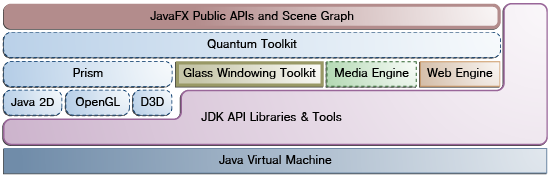
\includegraphics[scale=0.7]{Gambar/arsitekturJavaFX}
	\caption{Arsitektur JavaFX}
	\end{figure}
	
Ilustrasi dari gambar \textbf{2.1} mendeskripsikan setiap komponen saling berhubungan. Dibawah JavaFX Public API terdapat mesin yang menjalankan code JavaFX. Mesin tersebut terdiri dari sub komponen termasuk mesin grafis berperforma tinggi yang dinamakan Prism. Selain itu, terdapat sistem \textit{windowing} kecil dan efisien yang dinamakan Glass. Terakhir dalam mesin dibawah JavaFX Public API terdapat sebuah \textit{media engine} dan \textit{web engine}. Berikut ini elemen-elemen yang terdapat pada arsitektur JavaFX : \cite{javafx}
\begin{enumerate}
	\item \textit{Scene Graph}
	\item Java Public API untuk Fitur JavaFX
	\item \textit{Graphics System}
	\item \textit{Glass Windowing Toolkit}
	\item Gambar dan Media
	\item Komponen Web
	\item CSS
	\item \textit{UI Control}
	\item Layout
	\item Transformasi 2-D dan 3-D
	\item \textit{Visual Effecs}
\end{enumerate}

\subsection{Scene Graph}
\label{subs:Scene_Graph}
\textit{Scene Graph} merupakan sebuah pohon hirarki dari sekumpulan node yang merepresentasikan elemen visual dari antarmuka suatu aplikasi. Sebuah elemen dari \textit{scene graph} dinamakan node. Setiap node mempunya ID, \textit{style class} dan \textit{boundling volume}. Node dalam \textit{scene graph} juga memiliki :\cite{javafx}
\begin{enumerate}
	\item \textit{Effect}, seperti blur dan shadow
	\item \textit{Opacity}
	\item \textit{Transform}
	\item \textit{Event handler} (Mouse, keyboard, dan input method lainnya)
	\item Perintah spesifik dari sebuah aplikasi
\end{enumerate} 

Penggunaan \textbf{javafx.scene} API memungkinkan \textit{developer} untuk menggunakan beberapa jenis konten dialamnya, seperti : \cite{javafx}
\begin{enumerate}
	\item \textbf{Node} : Bentuk(2-D dan 3-D), gambar, media, \textit{embedded web browser}, teks, \textit{UI control}, grafik, grup, dan \textit{container}.
	\item \textbf{State} : Transformasi (posisi dan orientasi dari node), efek visual, dan konten visual lainnya.
	\item \textbf{Effect} : objek sederhana yang dapat merubah penampilan dari node \textit{scene graph}, seperti blur, shadow, dan \textit{color adjustment}
\end{enumerate}

\subsection{Java Public API untuk Fitur JavaFX}
\label{subs:API}
Pada lapisan atas arsitektur JavaFX pada gambar \textbf{2.1} API Java memberikan kebebasan dan fleksibilitas untuk membangun berbagai \textit{client} dari sebuah aplikasi. Platform JavaFX menggabungkan kemampuan terbaik yang dimiliki platform Java secara menyeluruh dan mendalam serta intuitif dengan memasukan fungsi media kedalamnya, sehingga tercipta lingkup konsep \textit{one-stop development}. Berikut contoh kegunaan Java API untuk fitur JavaFX :\cite{javafx}
\begin{enumerate}
	\item Memungkinkan penggunaan fitur Java yang poweful seperti \textit{generics, annotations, multithreading}.
	\item Lebih mudah mengembangan web menggunakan JavaFX dibanding \textit{JVM-base dynamic languages} lainnya seperti Grovvy, dan JavaScript.
	\item Memungkinkan Java developer untuk menggunakan bahasa sistem seperti Groovy untuk menulis file besar atau kompleks pada aplikasi JavaFX.
	\item Memungkinkan penggunaan binding.
	\item Menambahkan koleksi library Java dengan memasukan urutan dan memetakan perubahan sehingga memngukinkan aplikasi untuk menghubungkan antarmuka kedalam data model, mengamati perubahan pada data model, dan memperbarui kontrol UI yang sesuai dengan perubahan tersebut.   
\end{enumerate}

\subsection{Graphic System}
\label{subs:Graphic_System}
\textit{JavaFX Graphic System} pada gambar \textbf{2.1} merupakan implementasi dari JavaFX \textit{scene graph layer}. Sistem grafis pada JavaFX mendukung tampilan 2-D dan 3-D, selain itu sistem grafis ini menyediakan \textit{software rendering} untuk mendukung akselerasi \textit{rendering} dari \textit{hardware}. Berukut ini merupakan dua \textit{graphic accelerated pipeline} yang ada pada JavaFX platform :\cite{javafx}
\begin{enumerate}
	\item \textbf{Prism} yang bekerja pada proses render. Prism dapat bekerja pada kedua sisi baik \textit{hardware} maupun \textit{software} rendering termasuk 3-D rendering. Prism juga bertanggung jawab untuk proses \textit{rasterization}(mengubah vektor menjadi pixel atau dot) dan rendering pada JavaFX.
	\item \textbf{Quantum Toolkit} merupakan perpaduan Prism dan Windowing Toolkit yang bekerja di lapisan teratas pada JavaFX untuk mengatur \textit{threading rule} yang berhubungan dengan rendering dan \textit{event handling}. 
\end{enumerate}

\subsection{Glass Windowing Toolkit}
\label{subs:Glass_Windowing_Toolkit}
Tugas pada lapisan ini adalah membantu \textit{service} pada sistem operasi, seperti mengatur windows, waktu , dan \textit{surface}. Glass Toolkit juga bertanggung jawab atas pengaturan \textit{event queue}.\cite{javafx}

\subsection{Media dan Gambar}
\label{subs:Media_Gambar}
Fungsi -fungsi media pada JavaFX tersedia pada \textbf{javafx.scene.media} API. JavaFX mensuport baik visual maupun audio. Beberapa format yang disuport seperti MP3, AIFF, WAV pada file audio dan format FLV pada video. Ada tiga komponen yang berperan pada JavaFX media, yaitu :\cite{javafx} 
\begin{enumerate}
	\item \textit{Media object} merepresentasikan sebuah file media.
	\item \textit{Media Player} memutar sebuah file media.
	\item \textit{Media View} merupakan sebuah node yang menampilkan media tersebut.
\end{enumerate}

\subsection{Komponen Web}
\label{subs:Komponen_Web}
Mesin Web pada JavaFX merupakan bagian dari JavaFX UI control yang berbasis Webkit, dimana mesin web ini dapat menampilkan sebuah website dan melakukan browsing melalui APInya. Berikut ini fitur JavaFX yang dapat di implementasikan pada program java :\cite{javafx}
\begin{enumerate}
	\item Render konten HTML dari local atau remote URL.
	\item Mendukung history dan menyediakan navigasi Back dan Forward.
	\item \textit{Reload Content}.
	\item Edit konten HTML.
	\item Mengeksekusi perintah JavaScript.
	\item \textit{Handle event}.
\end{enumerate} 

Komponen dari browser tersebut terbagi kedalam ke kelas-kelas berikut :\cite{javafx}
\begin{enumerate}
	\item \textbf{WebEngine} : menyediakan kemampuan dasar dari halaman web.
	\item \textbf{WebView} : merangkum sebuah \textit{WebEngine object}, Menggabungkan konten HTML kedalam layar aplikasi, dan mendukung \textit{field} dan \textit{method} untuk menerapkan efek dan transformasi berupa ekstensi maupun sebuah kelas Node.
\end{enumerate}

\subsection{CSS}
\label{subs:CSS}
JavaFX Cascading Style Sheet (CSS) mendukung kemampuan untuk mengkustom styling pada antarmuka sebuah aplikasi JavaFX tanpa merubah \textit{source code} aplikasi tersebut.\cite{javafx}   

\subsection{UI Control}
\label{subs:UI_Control}
JavaFX UI Control dalam JavaFX API dibangun menggunakan node pada scene graph. JavaFX UI Control dapat mengambil keuntungan dari fitur yang diberikan platform JavaFX dan bersifat \textit{portable} pada platform yang berbeda.\cite{javafx}

\begin{figure}[H]
	\centering
	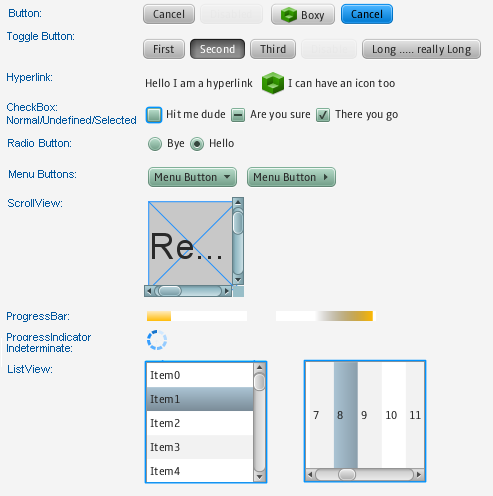
\includegraphics[scale=0.8]{Gambar/JavaFXuicontrols}
	\caption{Contoh JavaFX UI Control}
	\end{figure}
	
	pada gambar \textbf{2.2} menunjukan UI Control yang sementara didukung oleh JavaFX. Java UI control baru seperti TitlePane atau Accordion sebelumnya telah diperkenalkan pada JavaFX SDK. UI control tersebut terdapat pada \textbf{javafx.scene.control} \textit{package}.\cite{javafx}
 
\subsection{Layout}
\label{subs:Layout}
 \textit{Layout container} atau panel digunakan untuk pengatruan UI control secara dinamis dan fleksibel dalam scene graph pada aplikasi JavaFX. JavaFX Layout API mempunyai kelas-kelas yang dapat mengotomatiskan tata letak model sebagai berikut:\cite{javafx}
\begin{enumerate}
	\item \textbf{BorderPane} merupakan kelas yang mengatur bagian atas, bawah, kiri, kanan layout.
	\item \textbf{Hbox} merupakan kelas yang mengatur konten node secara horizontal dalam satu baris.
	\item  \textbf{Vbox} merupakan kelas yang mengatur konten node secara vertikal dalam satu baris.
	\item \textbf{StackPane} adalah kelas yang menempatkan \textit{back-to-front} konten node pada suatu \textit{stack}.
	\item \textbf{GridPane} adalah kelas yang memungkinkan developer untuk membuat sebuah grid baris dan kolom secara flexible untuk memetakan konten node.
	\item \textbf{FlowPane} adalah kelas yang mengatur alur konten node baik horizontal maupun vertical, \textit{wrapping} pada batas lebar konten (untuk horizontal) atau tinggi konten (untuk vertical).
	\item \textbf{AnchorPane} adalah kelas yang memungkinkan developer untuk membuat \textit{anchor} node pada layout atas, bawah, sisi kiri atau ditengah layout. 
\end{enumerate}

\subsection{Transformasi 2-D dan 3-D}
\label{subs:Layout}
Setiap node pada JavaFX scene graph dapat ditransformasikan dalam koordinat x-y melalui kelas-kelas \textit{javafx.scene.transform} berikut ini:\cite{javafx}
\begin{enumerate}
	\item \textbf{translate} - Memindahkan sebuah node dari satu posisi ke posisi lain bersama koordinat x,y,z yang relatif terhadap posisi awalnya.
	\item \textbf{scale} - Meresize sebuah node untuk membesar atau mengecil sesuai koordinat x,y,z tergantung skala faktornya.
	\item \textbf{rotate} - Merotasi sebuah node sesuai titik porosnya.
	\item \textbf{affine} - Melakukan pemetaan linear dari koordinat 2-D / 3-D ke koordinat 2-D / 3-D lainnya dengan menjaga lurus dan paralel sifat garis tersebut. Kelas ini digunakan bersamaan dengan kelas lainya dibanding penggunaan langsung.
\end{enumerate}

\subsection{Komponen JavaFX}
\label{subs:Komponen_Java_FX}
Berikut ini merupakan kumpulan \textit{package} yang ada dalam JavaFX.\cite{javafx3}
\begin{table}[H]
		\centering
		\caption{Tabel komponen JavaFX}
		\label{tab:komponen_javafx}
	\begin{tabular}{|c|p{12cm}|}
		\hline
		\textbf{No} & \textbf{Package dan Deskripsi} \\ \hline \hline
		1 & \textbf{javafx.application}\\
			&	Menyediakan kelas-kelas dalam siklus aplikasi.\\ \hline
		2 & \textbf{javafx.event}\\
			&	Memberikan kerangka dasar untuk FX event, dari mulai pengiriman hingga handling.\\ \hline	
		3 & \textbf{javafx.fxml}\\
			&	Berisi kelas untuk membuat hirarki objek dari markup.\\ \hline
		4 & \textbf{javafx.scene}\\
			&	Memberikan set basis kelas - kelas untuk JavaFX Scene Graph API .\\ \hline
		5 & \textbf{javafx.scene.control}\\
			&	JavaFX \textit{User Interface Control }(kontrol UI atau kontrol saja) dimana node khusus dalam JavaFX Scenegraph yang dapak digunakan untuk banuak konteks aplikasi yang berbeda.\\ \hline
		6 & \textbf{javafx.scene.input}\\
			&	Menyediakan set kelas - kelas untuk mouse dan keyboard \textit{input event handling}.\\ \hline
		7 & \textbf{javafx.scene.layout}\\
			&	Menyediakan kelas - kelas untuk mendukung UI layout.\\ \hline
		8 & \textbf{javafx.scene.text}\\
			&	Menyediakan set kelas - kelas untuk font dan teks node yang dapat di render.\\ \hline
		9 & \textbf{javafx.util}\\
			&	Berisi berbagai utilitas dan kelas pembantu.\\ \hline
		10 & \textbf{javafx.util.converter}\\
			&	\textit{Package} ini untuk konversi String pada JavaFX.\\ \hline
		11 & \textbf{javafx.beans}\\
			&	\textit{Package} ini berisi interface yang mendefinisikan bentuk umum dari \textit{observability}.\\ \hline
		12 & \textbf{javafx.beans.binding}\\
			&	\textit{Package} ini untuk menjelaskan karakter dari \textit{Binding}.\\ \hline	
		13 & \textbf{javafx.beans.value}\\
			&	\textit{Package} ini berisi fundamental interface dari \textit{observableValue} dan \textit{WritebleValue} dan semua sub interface di dalamnya.\\ \hline
		14 & \textbf{javafx.collections}\\
				&	\textit{Package} ini berisi koleksi penting dari javaFX dan koleksi utilitas lainnya.\\ \hline						
	\end{tabular}
\end{table}
\subsection{Property}
Properti merupakan \textit{interface} generik yang mendefinisikan metode umum untuk sifat yang dapat ditulis secara independen sesuai tipenya.\cite{javafx3}
\subsection{javafx.collections}
\subsubsection{ObservableList}
Dalam \textit{package} javafx.collections terdapat sebuah \textit{interface} yang bernama ObservableList. \textit{Interface} ini merupakan sebuah \textit{list} yang memungkinkan \textit{listeners} melacak ketika terjadi perubahan pada \textit{list} tersebut.
. Berikut ini \textit{method} yang ada pada \textit{interface} ObservableList.\cite{javafx3}
\begin{table}[H]
		\centering
		\caption{Tabel method ObservableList}
		\label{tab:method_ObservableList}
	\begin{tabular}{|c|p{12cm}|}
		\hline
		\textbf{No} & \textbf{Method dan Deskripsi} \\ \hline \hline
		1 & \textbf{addAll(E... elements)}\\
			&	Sebuah metode untuk menambah semua variabel dari sebuah elemen.\\ \hline
		2 & \textbf{addListener(ListChangeListener<? super E> listener)}\\
			&	Menambahkan \textit{listeners} pada sebuah observableList.\\ \hline
	\end{tabular}
\end{table}

\subsubsection{ListChangeListener}
\textit{Interface} ini menerima informasi perubahan dari sebuah ObservableList. Berikut ini \textit{method} yang ada pada \textit{interface} ListChangeListener.\cite{javafx3}
\begin{table}[H]
		\centering
		\caption{Tabel method ListChangeListener}
		\label{tab:method_ListChangeListener}
	\begin{tabular}{|c|p{12cm}|}
		\hline
		\textbf{No} & \textbf{Method dan Deskripsi} \\ \hline \hline
		1 & \textbf{onChanged(ListChangeListener.Change<? extends E> c)}\\
			&	Metode ini dipanggil ketika perubahan telah dilakukan terhadap sebuah ObservableList.\\ \hline
	\end{tabular}
\end{table}

\subsection{javafx.scene.control}
JavaFX UI \textit{control}(kontrol UI atau Kontrol) merupakan Node khusus pada JavaFX \textit{scenegraph} yang dapat digunakan berulang kali menyesuaikan kebutuhan rancangan aplikasi. Kontrol UI dapat disesuaikan visualnya oleh desainer atau pengembang aplikasi. \textit{Interface} ini didesain untuk berkerja dalam \textit{layout system}. Contoh \textit{interface} ini adalah Button, Label, ListView, TableView, dan TextField.\cite{javafx3}

\subsubsection{TextField}
TextField merupakan komponen \textit{input} teks yang memungkinkan pengguna untuk memasukan satu baris teks terformat. Berikut ini \textit{method} pada kelas TextField.\cite{javafx3}
\begin{table}[H]
		\centering
		\caption{Tabel method TextField}
		\label{tab:method_textField}
	\begin{tabular}{|c|p{12cm}|}
		\hline
		\textbf{No} & \textbf{Method dan Deskripsi} \\ \hline \hline
		1 & \textbf{getOnAction()}\\
			&	Metode ini menangani aksi terkait \textit{text field} ini. Method ini mengembalikan nilai null bila tidak ada aksi yang diberikan.\\ \hline
	\end{tabular}
\end{table}

\subsubsection{TableView}
TableView dirancang untuk memvisualisasikan jumlah baris data. Jumlah baris data tersebut akan dipecah menjadi kolom-kolom dalam TabelView. Berikut \textit{method} dalam kelas TabelView.\cite{javafx3}

\begin{table}[H]
		\centering
		\caption{Tabel method TabelView}
		\label{tab:method_TabelView}
	\begin{tabular}{|c|p{12cm}|}
		\hline
		\textbf{No} & \textbf{Method dan Deskripsi} \\ \hline \hline
		1 & \textbf{setItems(ObservableList<S> value)}\\
			&	Menetapkan nilai dari properti item pada tabel.\\ \hline
		2 & \textbf{getOnSort()}\\
			&	\textit{Method} ini dipanggil ketika ada permintaan untuk \textit{sorting}.\\ \hline		
	\end{tabular}
\end{table}

\subsubsection{TableColumn}
Sebuah TableView terdiri dari sejumlah TableColumn. Setiap TableColumn pada tabel bertanggung jawab menampilkan dan mengedit isi kolom. Berikut \textit{method} pada TableColumn.\cite{javafx3}
\begin{table}[H]
		\centering
		\caption{Tabel method TableColumn}
		\label{tab:method_TableColumn}
	\begin{tabular}{|c|p{14cm}|}
		\hline
		\textbf{No} & \textbf{Method dan Deskripsi} \\ \hline \hline
		1 & \textbf{setCellValueFactory(Callback<TableColumn.CellDataFeatures<S,T>}\\
			& \textbf{,ObservableValue<T>> value)}\\
			&	Menetapkan nilai properti \textit{CellFactory} yang dibutuhkan untuk menentukan bagaimana sel terisi pada satu TableColumn .\\ \hline	
	\end{tabular}
\end{table}
}{}
\ifdefstring{\vbabc}{1}{ \chapter{Analisis}
\label{chap:analysis}
Pada bab ini, akan dijelaskan mengenai analisis \textit{input} dan fitur perangkat lunak, deskripsi pengguna perangkat lunak,  pengembangan perangkat lunak, \textit{use case} dari perangkat lunak serta diagram aktifitas dari perangkat lunak.
\section{Analisis Input}
\subsection{Analisis File Excel Jadwal Mengawas Ujian}
Sub bab ini akan membahas analisis file excel yang dikeluarkan oleh TU(Tata Usaha).\\
TU FTIS mengeluarkan jadwal setiap semester yang dibagikan kepada dosen FTIS. 
berikut ini contoh file excel yang dikeluarkan oleh TU. 
\begin{figure}[H]
	\centering
	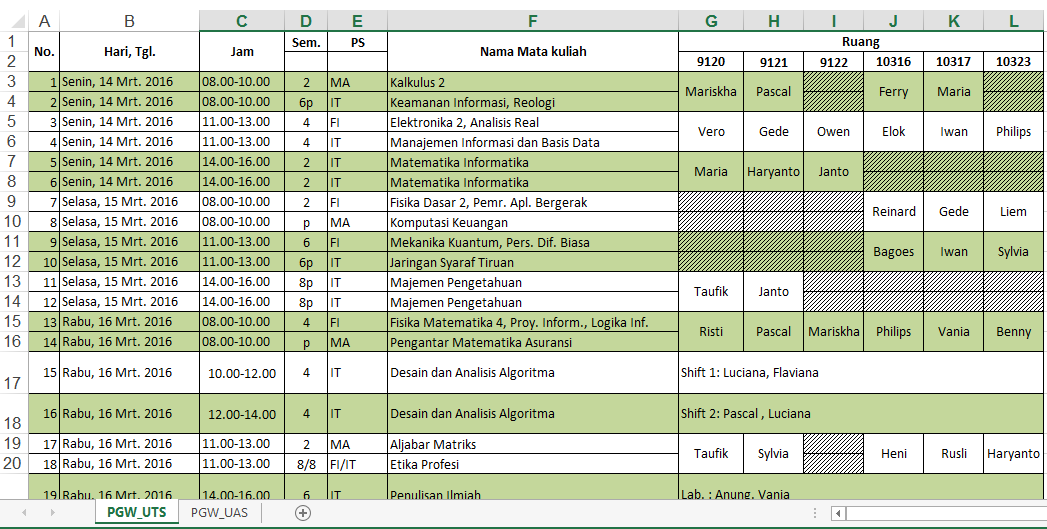
\includegraphics[scale=0.5]{Gambar/scJadwal}
	\caption{Jadwal mengawas ujian FTIS}
	\label{fig:jadwalLamapng}
	\end{figure}

Berikut penjelasan kolom-kolom yang ada di gambar \ref{fig:jadwalLamapng}.\\
File excel jadwal mengawas ujian yang dipublikasikan Tata Usaha FTIS yang terdiri dari 12 kolom A sampai dengan L.
Tabel ~\ref{tab:penjelasan_kolom} menjelaskan rincian dari masing-masing kolom pada excel tersebut. 
\begin{table}[H]
		\centering
		\caption{Tabel penjelasan kolom pada excel mengawas ujian}
		\label{tab:penjelasan_kolom}
\begin{tabular}{|c|p{12cm}|}
		\hline
		\textbf{No} & \textbf{Kolom dan Deskripsi} \\ \hline \hline
		1 & \textbf{No}\\
			&	Menyatakan nomer urut jadwal mengawas ujian.\\ \hline
		2 & \textbf{Hari, Tanggal}\\
			&	Kolom dalam bentuk String berisi hari dan tanggal. Terdapat singkatan yang diberikan TU dalam contoh ini  Mrt. menunjukan bulan Maret\\ \hline	
		3 & \textbf{Jam}\\
			&	Kolom ini bertipe String dan menerangkan pukul dilaksakannya mengawas ujian.\\ \hline
		4 & \textbf{Semester}\\
			&	Kolom ini bertipe String dan mengerangkan semester dari mata kuliah yang diujiankan . Terdapat simbol p yang menerangkan matakuliah pilihan\\ \hline
		5 & \textbf{PS}\\
			&	Bertipe string berisi program studi yang terkait dengan ujian mata kuliah tersebut.\\ \hline
		6 & \textbf{Nama Mata Kuliah}\\
			&	Kolom bertipe String dan berisi tentang mata kuliah yang diujiankan.\\ \hline
		7 & \textbf{Ruangan}\\
			&	Kolom dengan merge 6 kolom dan pada baris kedua terdapat 6 kolom ruangan ujian yaitu 9120, 9121, 9122, 10316, 10317, 10323. Masing kolom ruangan berisi nama pengawas ujian bertipe String. Ruangan tidak terpakai ditandai dengan garis-garis miring. Jika ada isi kolom ruangan yang dimerge sebanyak 6 kolom menandakan ruangan tersebut adalah laboratorium komputer FTIS.\\ \hline
	\end{tabular}	
\end{table}

Dari rincian tabel ~\ref{tab:penjelasan_kolom} berikut analisis \textit{flowchart} cara perangkat lunak membaca file excel : 
\begin{figure}[H]
	\centering
	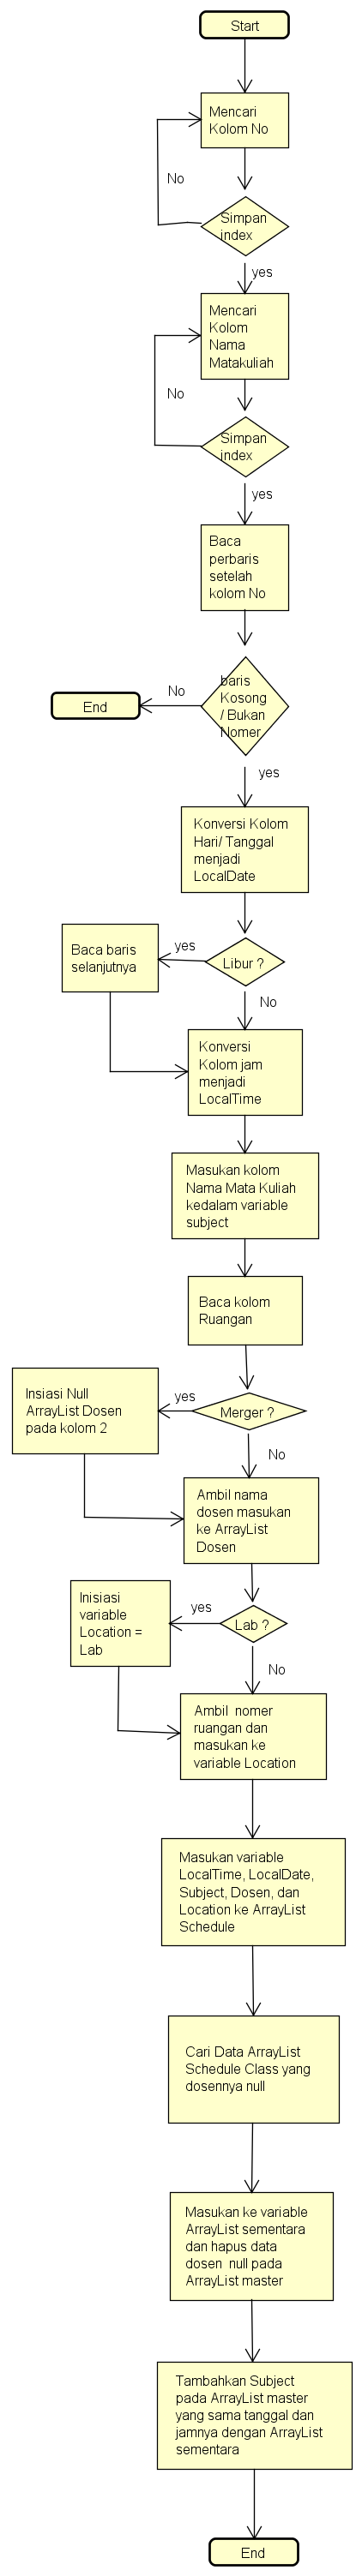
\includegraphics[scale=0.3]{Gambar/FlowchartBacaExcel}
	\caption{\textit{Flowchart} membaca excel}
	\label{fig:flowchartMembacaExcel}
	\end{figure}
\begin{enumerate}
	\item Kolom \textbf{No.} dapat dijadikan acuan dalam membaca baris jadwal Excel pada perangkat lunak. Jika PL menemukan kolom No pada excel maka simpan baris dan kolomnya pada variabel tertentu untuk menandakan bahwa baris selanjutnya merupakan data yang dibutuhkan oleh perangkat lunak. Selanjutnya nomer pada kolom No. juga dapat dijadikan penanda dalam perangkat lunak menentukan banyak data yang dibaca, jika baris selanjutnya dari kolom No. merupakan angka maka dipastikan baris tersebut memuat data jadwal mengawas.
		\item Kolom \textbf{Hari, Tgl.} memuat tanggal dan hari ujian menggunakan koma (,) sebagai pemisah hari dan tanggal dan titik (.) sebagai penanda singkatan bulan. Untuk mendapatkan tanggal yang sesuai dengan format \textit{LocalDate} maka perangkat lunak harus melakukan \textit{parsing} memisahkan hari dengan tanggal, kemudian mengkonversi bulan menjadi sebuah angka sehingga sesuai dengan format \textit{LocalDate}, lalu disimpan pada sebuah variabel.
		\item Kolom \textbf{Jam} menggunakan \textit{hyphen}(-) sebagai pemisah antara jam dimulainya ujian dan waktu ujian berakhir. perangkat lunak dapat melakukan \textit{parsing} untuk memisahkan waktu tersebut menjadi dua variabel, lalu dikonversi sesuai dengan ketentuan \textit{LocalTime}.
		\item Kolom \textbf{Nama Mata kuliah} memuat nama mata kuliah yang diujiankan, karena satu dosen dapat mengawas salah satu dari 2 matakuliah sehingga pada kolom ruangan yang memuat dua matakuliah yang ditandai dengan \textit{merger} dua baris yang berisi nama pengawas ujian.
		\item kolom \textbf{Ruangan} pada kolom ini terdapat 6 ruangan yang masing-masing kolom dan baris akan disimpan pada varible untuk dicocokan nanti pada saat membaca file excel satu per satu untuk menentukan lokasi ujian tersebut berlangsung.
		\item Jika perangkat lunak menemukan kata \textit{LIBUR} atau menemukan mata kuliah yang tidak ada dosen pengawasnya maka baris tersebut akan dilewati menuju baris selanjutnya.
		\item Jika perangkat lunak menemukan kata \textit{Shift} atau \textit{Lab} maka otomatis perangkat lunak akan menginisiasi tempat berlangsungnya ujian adalah Laboratorium Komputer.
		\item Semua variabel LocalDate, LocalTime, \textit{subject}, dosen, dan \textit{location} yang telah terisi kemudian dimasukan ke dalam sebuah ArayList \textit{schedule}.
		\item ArrayList \textit{schedule} kemudian diperiksa kembali sehingga jika pada data excel dosen memiliki 2 jadwal mengawas, maka pada ArrayList \textit{schedule} satu dosen tersebut memiliki 2 \textit{subject}.
		\item Poses ini menghasilkan \textit{output} berupa sebuah ArrayList \textit{schedule} yang memuat semua data file excel jadwal mengawas ujian yang telah dikonversi dan distandarisasi. 
\end{enumerate}

Selanjutnya adalah analisis berupa wawancara dengan dosen mengenai jadwal mengawas ujian. Hasilnya dosen FTIS tidak memerlukan kolom semseter dan program studi pada file excel jadwal mengawas. Hal ini disebabkan karena dosen FTIS dapat saling mengawas ujian antar program studi selama program studi tersebut masih dalam lingkup FTIS.Dari analisis tersebut maka kolom yang butuhkan untuk ditampilkan pada PL, yaitu :
\begin{table}[H]
		\centering
		\caption{Tabel analisa kolom pada excel mengawas ujian}
		\label{tab:analisa_kolom}
\begin{tabular}{|c|p{12cm}|}
		\hline
		\textbf{No} & \textbf{Kolom dan Deskripsi} \\ \hline \hline
		1 & \textbf{Hari, Tanggal}\\
			&	Kolom ini bertipe String dan terdapat singkatan seperti Mrt, maka akan dibuatkan fungsi pada saat implementasi agar seragam dan sesuai dengan format tgl dan waktu pada Java.\\ \hline	
		2 & \textbf{Jam}\\
			&	Kolom ini bertipe String, maka dibutuhkan konversi String kedalam fungsi jam pada saat implementasi.\\ \hline
		3 & \textbf{Nama Mata Kuliah}\\
			&	Kolom ini dapat menerangkan deskripsi mata kuliah pada PL.\\ \hline
		4 & \textbf{Dosen}\\
			&	Kolom ini merupakan isi dari tabel kelas pada excel, pada PL akan ditampilkan sebagai kolom tersendiri menerangkan nama pengawas ujian.\\ \hline		
		7 & \textbf{Ruangan}\\
			&	Kolom ini akan berisi ruangan ujian, mata kuliah, waktu dan tanggal.\\ \hline
	\end{tabular}
\end{table}

\subsection{Flowchart Konversi ArrayList Jadwal ke iCalendar}
Setelah dibaca file excel akan berubah menjadi ArrayList \textit{schedule}, kemudian data list tersebut yang menjadi \textit{input} untuk dikonversi menjadi iCalendar. Berikut alur dari konversi tersebut :

\begin{figure}[H]
	\centering
	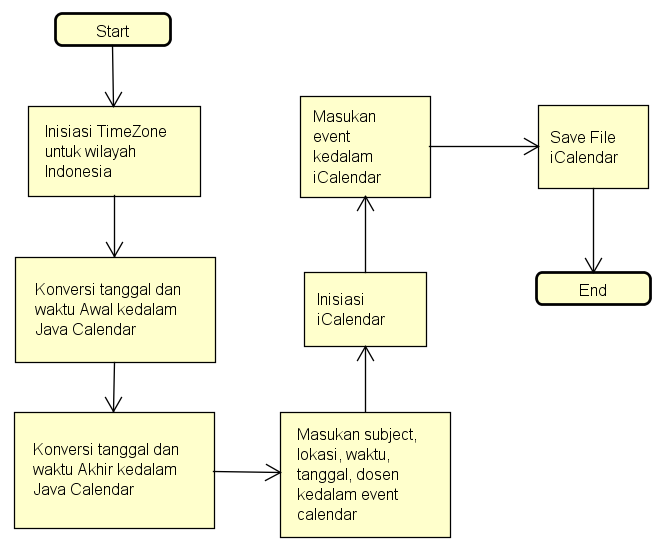
\includegraphics[scale=0.4]{Gambar/FlowchartConvertiCalendar}
	\caption{\textit{Flowchart} alur konversi excel ke iCalendar}
	\label{fig:flowchartKonversiiCalendar}
	\end{figure}
\begin{enumerate}
	\item Menginisiasi waktu indonesia.
	\item Mengkonversi waktu awal atau waktu masuk ujian kedalam format Java Calendar.
	\item Mengkonversi waktu akhir atau waktu selesai ujian kedalam format Java Calendar.
	\item Masukan mata kuliah/\textit{subject}, lokasi, jam, tanggal dari ArrayList jadwal kedalam variabel event Kalender.
	\item Inisiasi iCalendar.
	\item Masukan semua komponen event pada iCalendar.
	\item \textit{Output} icalendar dapat disimpan pada alamat folder yang diinginkan.
\end{enumerate}

\subsection{Analisis Kebutuhan Perangkat Lunak}
Perangkat Lunak ini akan memiliki fitur sebagai berikut : 
	\begin{enumerate}
		\item Perangkat lunak ini dapat menerima dan membaca\textit{input} file excel jadwal mengawas ujian yang dikeluarkan oleh TU FTIS.
		\item Perangkat lunak ini dapat mengubah file excel menjadi iCalendar.
		\item File iCalendar dapat diunduh oleh pengguna.
		\item Pengguna dapat melakukan \textit{sort} terhadap nama pengawas ujian.
	\end{enumerate}

\subsubsection{Deskripsi Pengguna}
Pengguna perangkat lunak ini merupakan dosen yang aktif mengajar di FTIS.
	
\section{Use Case Perangkat Lunak}

Berikut diagram use case berserta skenario yang tertera pada gambar \ref{fig:useCaseJadwal}

\begin{figure}[h]
	\centering
	\includegraphics[scale=0.5]{Gambar/useCaseJadwal}
	\caption{Diagram use case perangkat lunak konversi jadwal mengawas ujian}
	\label{fig:useCaseJadwal}
	\end{figure}

\begin{enumerate}
	\item Skenario Memasukan input file excel \\
	{\renewcommand\labelitemi{}
		\begin{itemize}
			\item Deskripsi		: Kegiatan memasukan input file excel.
			\item Aktor				: Pengawas
			\item Prakondisi	: -
			\item Skenario		:
				\begin{itemize}
					\item Pengawas memasukan file excel mengawas ujian yang diterbitkan oleh TU
				\end{itemize}
		\end{itemize}
		}
		
	\item Skenario Melakukan Sorting nama
	{\renewcommand\labelitemi{}
	\begin{itemize}
			\item Deskripsi		: Kegiatan mensorting jadwal mengawas.
			\item Aktor				: pengawas
			\item Prakondisi	: -
			\item Skenario		:
				\begin{itemize}
					\item Pengawas
					dapat melakukan sorting nama dari jadwal ujian yang telah berupa iCal sesuai nama yang di inginkan. 
				\end{itemize}
		\end{itemize}
		}
		
		\item Skenario Mengunduh File iCal 
		{\renewcommand\labelitemi{}
		\begin{itemize}
			\item Deskripsi		: Kegiatan Mengunduh file iCal.
			\item Aktor				: Dosen 
			\item Prakondisi	: -
			\item Skenario		:
				\begin{itemize}
					\item Pengawas mengunduh file iCal yang telah dikonversi oleh perangkat lunak.
				\end{itemize}
		\end{itemize}
		}
		
		\item Skenario Membaca File Excel
		{\renewcommand\labelitemi{}
		\begin{itemize}
			\item Deskripsi		: Membaca File Excel.
			\item Aktor				: System 
			\item Prakondisi	: File bertipe excel dan berekstensi .xlsx
			\item Skenario		:
				\begin{itemize}
					\item System membaca file excel jadwal mengawas ujian.
				\end{itemize}
		\end{itemize}
		}
		
		\item Skenario Membaca File Excel
		{\renewcommand\labelitemi{}
		\begin{itemize}
			\item Deskripsi		: Membaca File Excel.
			\item Aktor				: System 
			\item Prakondisi	: File bertipe excel dan berekstensi .xlsx .
			\item Skenario		:
				\begin{itemize}
					\item System membaca file excel jadwal mengawas ujian.
				\end{itemize}
		\end{itemize}
		}
		
		\item Skenario Konversi File Excel Menjadi ArrayList Jadwal
		{\renewcommand\labelitemi{}
		\begin{itemize}
			\item Deskripsi		: konversi file excel menjadi ArrayList Jadwal.
			\item Aktor				: System 
			\item Prakondisi	: File excel telah dimasukan.
			\item Skenario		:
				\begin{itemize}
					\item System mengkonversi file excel yang telah dibaca menjadi ArrayList jadwal.
				\end{itemize}
		\end{itemize}
		}
		
		\item Skenario Menampilkan Jadwal Ke Layar
		{\renewcommand\labelitemi{}
		\begin{itemize}
			\item Deskripsi		: Menampilkan jadwal ke layar.
			\item Aktor				: System 
			\item Prakondisi	: File excel telah dikonversi menjadi ArrayList jadwal
			\item Skenario		:
				\begin{itemize}
					\item System nampilkan jadwal yang telah dikonversi dalam bentuk TableView ke layar.
				\end{itemize}
		\end{itemize}
		}
		
		\item Skenario Menyusun Tabel Sesuai Nama Pengawas
		{\renewcommand\labelitemi{}
		\begin{itemize}
			\item Deskripsi		: Menyusun tabel sesuai nama pengawas.
			\item Aktor				: System 
			\item Prakondisi	: TextBox Sort telah diisikan nama pengawas
			\item Skenario		:
				\begin{itemize}
					\item System menyusun tabel sesuai dengan nama pengawas yang dimasukan oleh pengguna pada TextBox Sort.
				\end{itemize}
		\end{itemize}
		}
		
		\item Skenario Mengkonversi File Seleksi ke iCalendar
		{\renewcommand\labelitemi{}
		\begin{itemize}
			\item Deskripsi		: Mengkonversi file seleksi ke icalendars.
			\item Aktor				: System 
			\item Prakondisi	: Pengguna menyeleksi satu item pada tabel yang akan dikonversi menjadi iCalendar
			\item Skenario		:
				\begin{itemize}
					\item System mengkonversi item yang telah diseleksi oleh pengguna pada tabel menjadi iCalendar.
				\end{itemize}
		\end{itemize}
		}
		
		\item Skenario Menyimpan File iCalendar Pada Destinasi Folder
		{\renewcommand\labelitemi{}
		\begin{itemize}
			\item Deskripsi		: Menyimpan file iCalendar pada destinasi folder.
			\item Aktor				: System 
			\item Prakondisi	: Pengguna telah menentukan destinasi folder dan memasukan nama file iCalendar
			\item Skenario		:
				\begin{itemize}
					\item System menyimpan file iCalendar yang telah dikonversi sebelumnya pada destinasi folder yang dipilih oleh pengguna beserta nama filenya.
				\end{itemize}
		\end{itemize}
		}
\end{enumerate}

\section{Diagram Aktifitas}
Pada subbab ini akan dibahas mengenai prosedur setiap aktifitas dari perangkat lunak.

\subsection{Memasukan Excel Jadwal Mengawas Ujian}
Tahap ini merupakan tahap awal proses file input dimasukkan kedalam perangkat lunak dimana file input yang dimaksud merupakan excel jadwal yang dikeluarkan TU FTIS. Berikut step-step untuk memasukan excel kedalam perangkat lunak.
\begin{figure}[h]
	\centering
	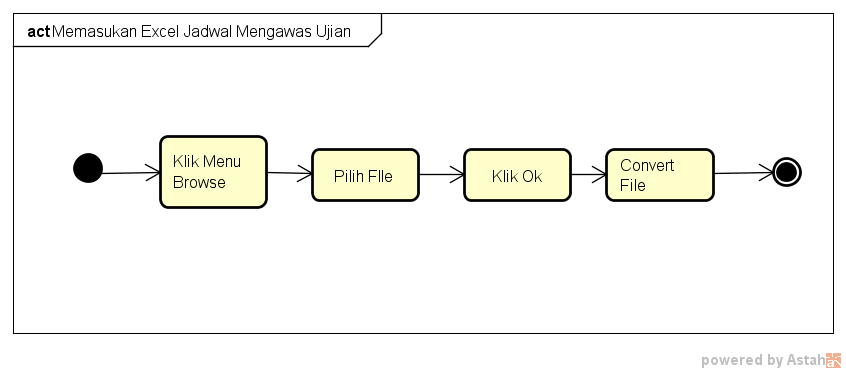
\includegraphics[scale=0.3]{Gambar/Memasukan-Excel-Jadwal-Mengawas-Ujian}
	\caption{Prosedur memasukan file excel jadwal mengawas ujian}
	\end{figure}
	
\begin{enumerate}
	\item Pengguna mengklik menu Browse yang ada di perangkat lunak. 
	\item Perangkat lunak menseleksi file yang berekstensi .xlsx yang dapat dipilih oleh pengguna.
	\item Pengguna memilih file excel yang akan dimasukkan.
	\item Pengguna mengklik tombol oke pada window.
	\item Pengguna mengklik tombol Convert untuk mengkonversi file excel.
	\item Perangkat lunak mengkonversi file excel menjadi ArrayList jadwal.
	\item Perangkat Lunak menampikan TableView jadwal yang telah dikonversi. 
\end{enumerate}

\subsection{Sorting Nama Pengawas}
Tahap ini menjelaskan bagaimana pengguna dapat memanfaatkan fitur dari perangkat lunak dengan mensorting nama dosen, dengan begitu jadwal pengawas yang dicari dapat diunduh dengan mudah. Berikut step-step untuk mensorting nama pengawas.
\begin{figure}[H]
	\centering
	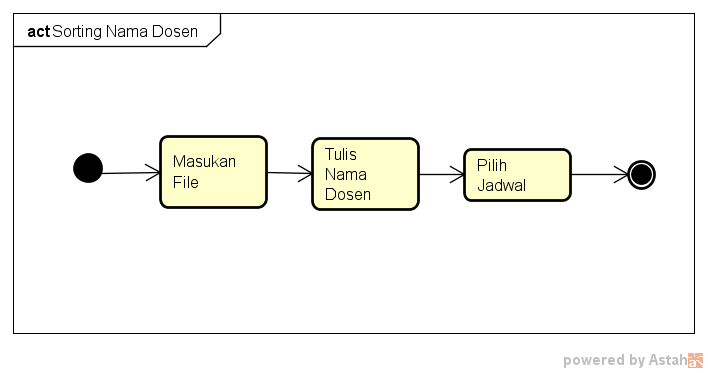
\includegraphics[scale=0.5]{Gambar/Sorting-Nama-Dosen}
	\caption{Prodsedur sorting nama pengawas}
	\end{figure}

\begin{enumerate}
	\item Pengguna menuliskan nama pengawas yang dicari.
	\item Perangkat lunak mencocokan nama pengawas dengan ArrayList jadwal.
	\item Data dengan nama pengawas yang sama akan disimpan pada ArrayList sementara.
	\item Atur kembali urutan tabel menggunakan ArrayList sementara lalu tampilkan ke pengguna.
\end{enumerate}

\subsection{Unduh File iCal}
Tahap ini merupakan tahap terakhir, file excel yang telah dimasukkan lalu dikonversi menjadi iCal selanjutnya pengguna tinggal memilih jadwal mana yang akan diunduh. File iCal yang telah dikonversi tersebut dapat diintegrasikan dengan aplikasi iCalendar seperti Google Calendar, Microsoft Outlook, dan Apple Calendar. Berikut step-step untuk mengunduh file iCal.
\begin{figure}[h]
	\centering
	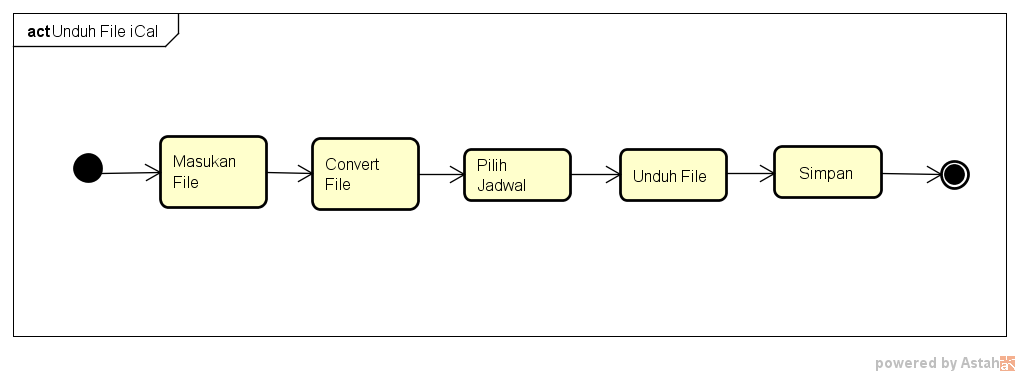
\includegraphics[scale=0.5]{Gambar/Unduh-File-iCal}
	\caption{Prosedur Mengunduh File iCal}
	\end{figure}

\begin{enumerate}
	\item Pengguna memilih jadwal yang akan dikonversi pada tabel.
	\item Pengguna mengklik tombol Convert to iCal pada perangkat lunak.
	\item Perangkat lunak mengkonversi jadwal yang dipilih oleh pengguna menjadi iCalendar.
	\item Pengguna menentukan destinasi folder penyimpanan dan menuliskan nama file iCalendar.
	\item Pengguna mengklik tombol simpan pada perangkat lunak.
\end{enumerate}

\section{Pemodelan Kelas}
Setelah file excel mengawas ujian tersebut dijabarkan dan dianalisis, pada subbab ini akan di jelaskan mengenai pembagian fungsi
kelas dalam rancangan perangkat lunak.

\subsubsection{Pemodelan Rancangan Kelas}
\begin{figure}[H]
	\centering
	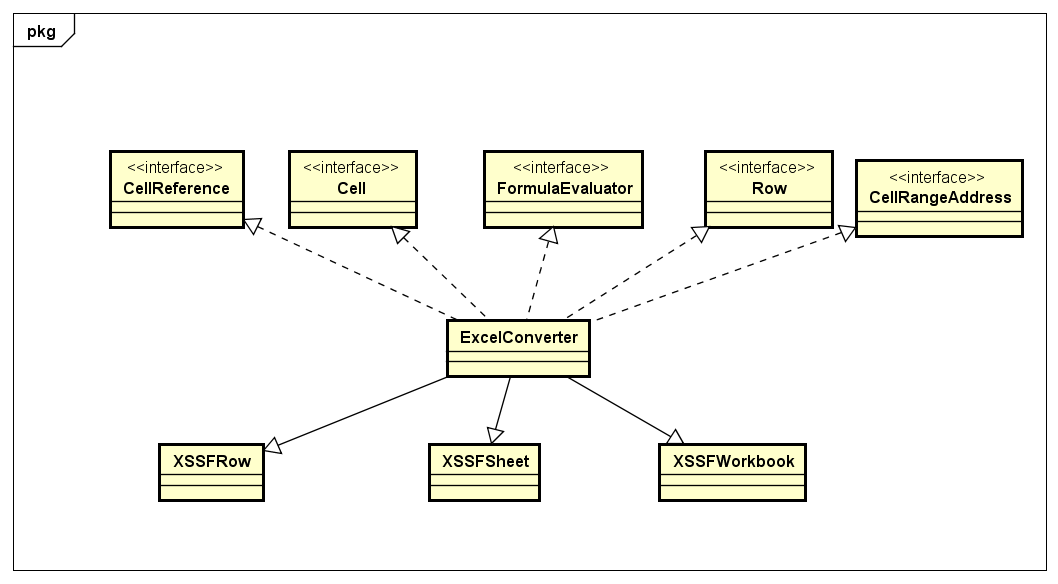
\includegraphics[scale=0.5]{Gambar/pemodelanExcelConverter}
	\caption{Gambar Pemodelan ExcelConverter}
	\label{fig:pemodelanExcelConverter}
\end{figure}

\begin{figure}[H]
	\centering
	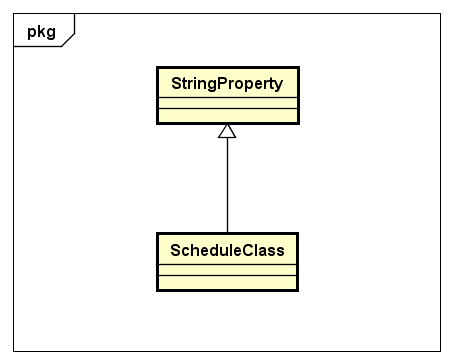
\includegraphics[scale=0.5]{Gambar/pemodelanScheduleClass}
	\caption{Gambar Pemodelan ScheduleClass}
	\label{fig:pemodelanExcelConverter}
\end{figure}

\begin{figure}[H]
	\centering
	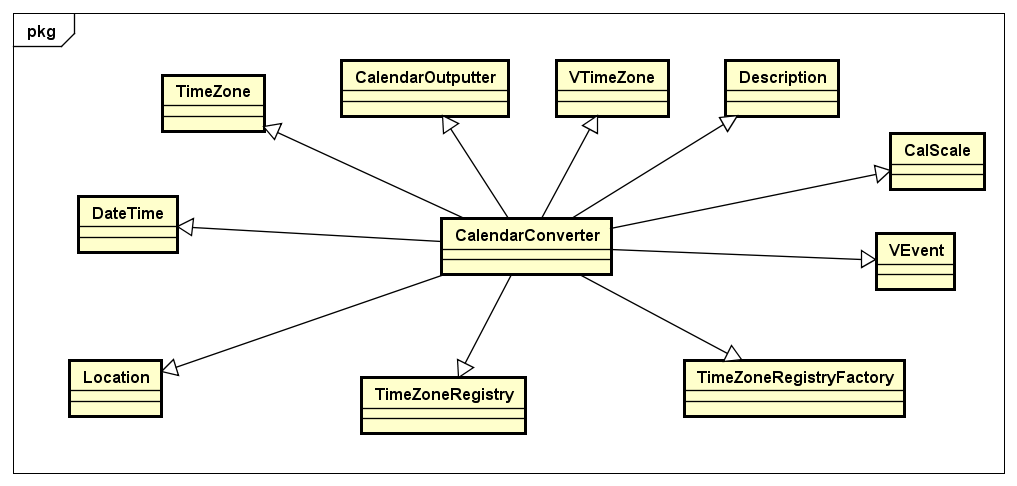
\includegraphics[scale=0.5]{Gambar/pemodelanCalendarConverter}
	\caption{Gambar Pemodelan CalendarConverter}
	\label{fig:pemodelanExcelConverter}
\end{figure}

\begin{figure}[H]
	\centering
	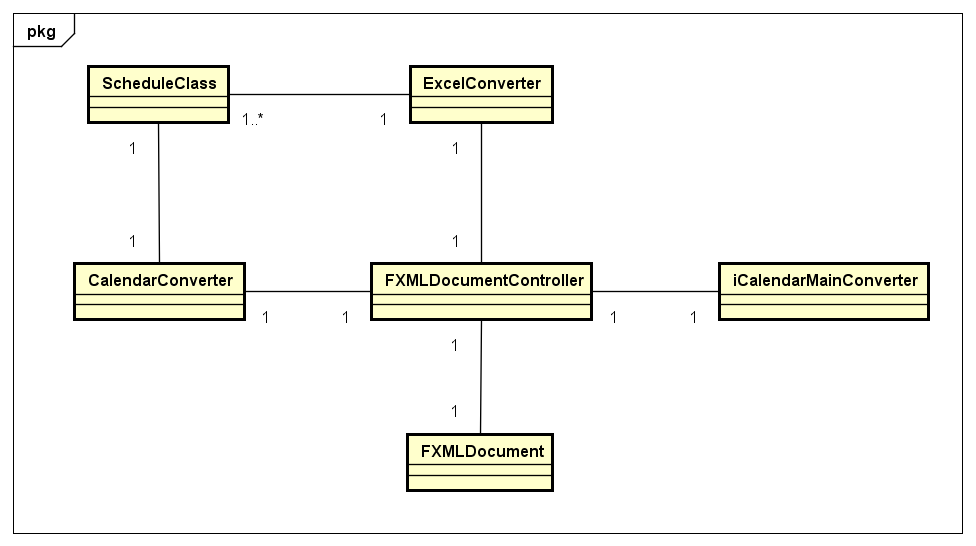
\includegraphics[scale=0.5]{Gambar/pemodelan-kelas}
	\caption{Gambar Pemodelan Kelas}
	\label{fig:pemodelanKelasSeluruh}
\end{figure}

Berikut penjelasan fungsi dari kelas dari gambar \ref{fig:pemodelanKelasSeluruh} :	
\begin{enumerate}
	\item \textbf{ScheduleClass}\\
	Kelas ini berfungsi menampung jadwal pengawas yang telah dikonversi oleh kelas ExcelConverter.
	\item \textbf{ExcelConverter}\\
	Kelas ini bertugas membaca file excel jadwal mengawas ujian sehingga dapat ditampilkan oleh perangkat lunak.
	\item \textbf{FXMLDocumentController}\\
	Kelas ini mempunyai peran untuk mendapatkan file \textit{input} yang dimasukkan oleh pengguna,  memberi perintah 
	kepada kelas ExcelConverter untuk membaca \textit{input}, menampilkannya kembali ke perangkat lunak dan memberikan perintah
	kepada CalendarConverter untuk mengkonversikannya dalam iCal.
	\item \textbf{CalendarConverter}\\
	Kelas ini berfungsi mengkonversi file yang telah dibaca kedalam format .ics atau iCalendar.
	\item \textbf{iCalendarMainConverter}\\
	kelas ini berfungsi sebagai \textit{main} pada perangkat lunak dimana kelas ini mengeksekusi dan menghubungkan seluruh elemen kelas 
	pada perangkat lunak ini.
\end{enumerate}
}{}
\ifdefstring{\vbabd}{1}{\chapter{Perancangan}
\label{chap:design}

Berdasarkan analisa dari bab 3, pada bab ini akan dibahas mengenai perancangan diagram kelas, dan perancangan antarmuka dari
program.

\section{Perancangan Diagram Kelas}
Berdasarkan hasil analisis dari bab 3, telah dijelaskan pemodelan struktur kelas yang akan digunakan pada program, selanjutnya pada subbab ini merupakan terjemahan dari pemodelan kelas dalam bentuk rancangan diagram kelas pada gambar ~\ref{fig:pemodelan-kelas}.   
\begin{figure}[H]
	\centering
	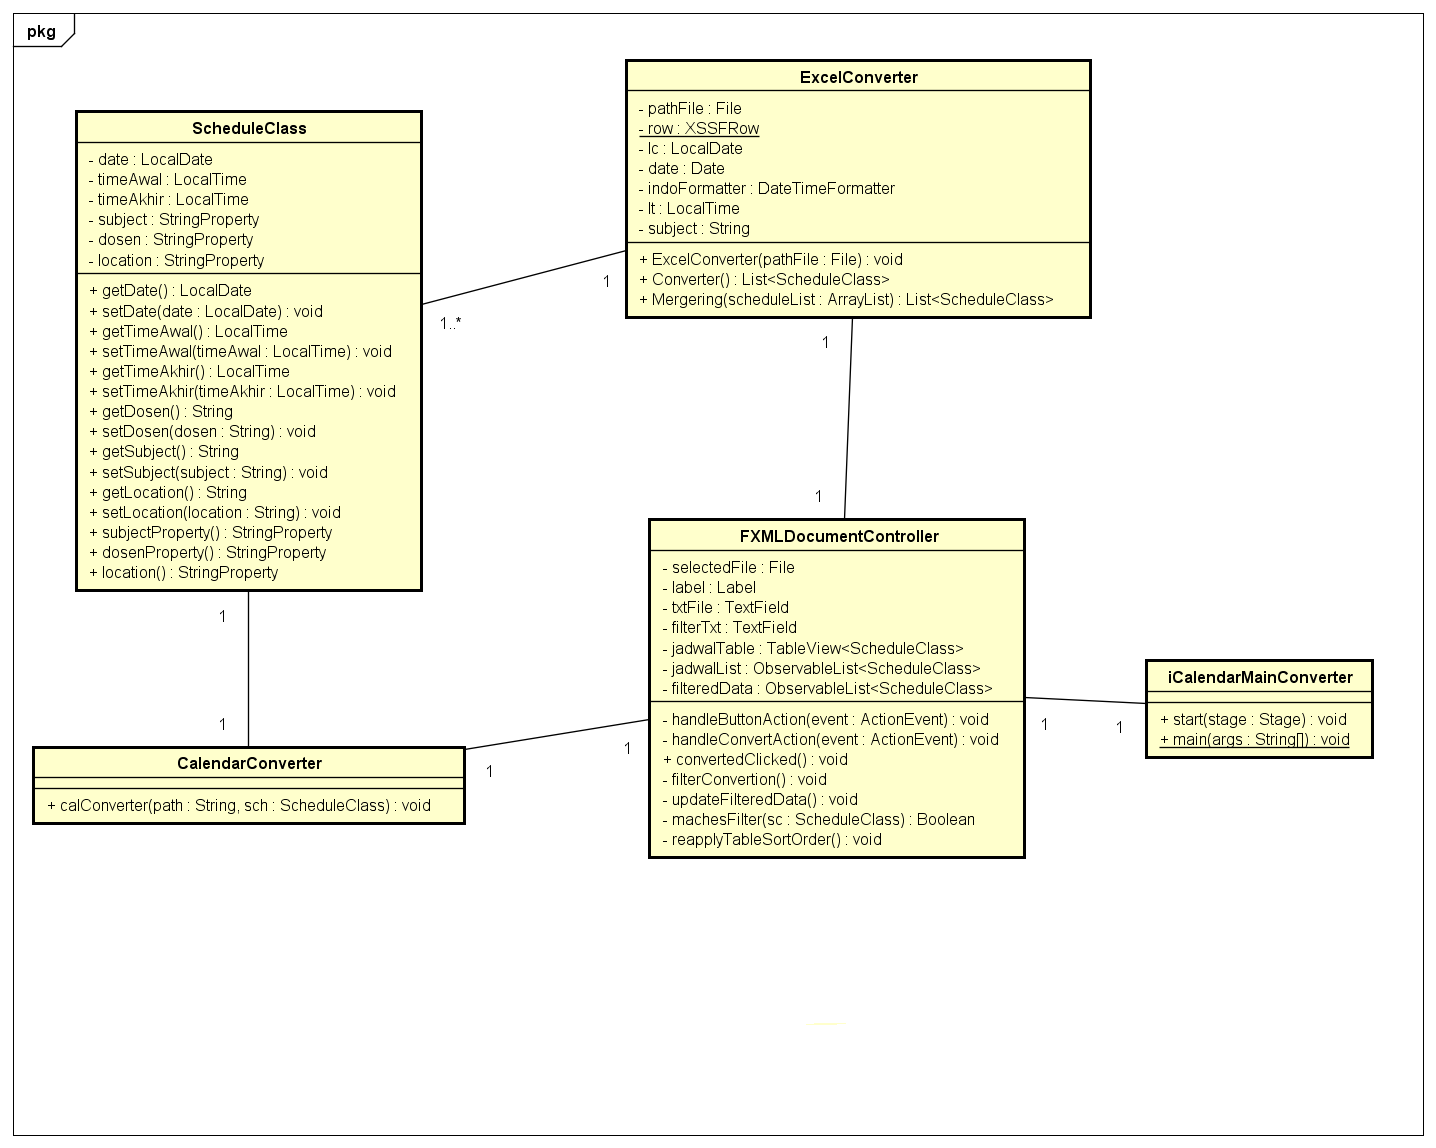
\includegraphics[scale=0.4]{Gambar/kelas-diagram}
	\caption{Gambar Kelas Diagram}
	\label{fig:pemodelan-kelas}
\end{figure}

Berikut ini rincian kelas pada diagram kelas yang tercantum dalam tabel-tabel dibawah ini :

\begin{table}[H]
	\centering
		\caption{Tabel Kelas \textit{ScheduleClass}}
		\label{tab:schedule_class}
		\begin{tabular}{ | c | c | c |}
			\hline
				\multicolumn{3}{|c|}{Atribut} \\ \hline 
				Nama atribut & Tipe Data  & Fungsi \\ \hline
				date & LocalDate & Atribut tanggal\\ \hline
				timeAwal & LocalTime & Atribut jam ujian dimulai\\ \hline
				timeAkhir & LocalTime & Atribut jam ujian berakhir\\ \hline
				subject & StringProperty & Atribut mata kuliah\\ \hline
				dosen & StringProperty & Atribut nama dosen\\ \hline
				location & StringProperty & Atribut lokasi ujian\\ \hline
				\multicolumn{3}{|c|}{Method} \\ \hline
				\multicolumn{2}{|c|}{Nama Method} & Fungsi \\ \hline
				\multicolumn{2}{|l|}{\textbf{getDate()}} & Mendapatkan tanggal\\ \hline
				\multicolumn{2}{|l|}{\textbf{setDate(date: LocalDate)}} & Set tanggal \\ \hline
				\multicolumn{2}{|l|}{\textbf{getTimeAwal()}} & Mendapatkan jam awal ujian \\ \hline
				\multicolumn{2}{|l|}{\textbf{setTimeAwal(timeAwal: LocalTime)}} & Set jam awal ujian\\ \hline
				\multicolumn{2}{|l|}{\textbf{getTimeAkhir()}} & Mendapatkan jam akhir ujian\\ \hline
				\multicolumn{2}{|l|}{\textbf{setTimeAkhir(timeAkhir: LocalTime)}} & Set jam akhir ujian\\ \hline
				\multicolumn{2}{|l|}{\textbf{getDosen()}} & Mendapatkan nama dosen\\ \hline
				\multicolumn{2}{|l|}{\textbf{setDosen(dosen: String)}} & Set nama dosen\\ \hline
				\multicolumn{2}{|l|}{\textbf{getSubject()}} & Mendapatkan nama mata kuliah\\ \hline
				\multicolumn{2}{|l|}{\textbf{setSubject(subject: String)}}& Set mata kuliah \\ \hline
				\multicolumn{2}{|l|}{\textbf{getLocation()}} & Mendapatkan lokasi ujian\\ \hline
				\multicolumn{2}{|l|}{\textbf{setLocation(location: String)}} & Set lokasi ujian\\ \hline
				\multicolumn{2}{|l|}{\textbf{subjectProperty()}} & Mendapatkan properti mata kuliah\\ \hline
				\multicolumn{2}{|l|}{\textbf{dosenProperty()}} & Mendapatkan properti dosen\\ \hline
				\multicolumn{2}{|l|}{\textbf{location()}} & Mendapatkan properti lokasi\\ \hline
		\end{tabular}
\end{table}

\begin{table}[H]
	\centering
		\caption{Tabel Kelas \textit{ExcelConverter}}
		\label{tab:excel_converter}
		\begin{tabular}{ | c | c | p{4cm} |}
			\hline
				\multicolumn{3}{|c|}{Atribut} \\ \hline 
				Nama atribut & Tipe Data  & Fungsi \\ \hline
				pathFile & File & Atribut path file excel mengawas\\ \hline
				row & XSSFRow & Atribut baris dari Excel\\ \hline
				lc & LocalDate & Atribut tanggal ujian\\ \hline
				indoFormater & DateTimeFormatter & Atribut konversi ke timezone jakarta\\ \hline
				lt & LocalTime & Atribut jam ujian\\ \hline
				subject & String & Atribut matakuliah\\ \hline
				\multicolumn{3}{|c|}{Method} \\ \hline
				\multicolumn{2}{|c|}{Nama Method} & Fungsi \\ \hline
				\multicolumn{2}{|c|}{\textbf{ExcelConverter(path: File)}} & Konstruktor untuk mendapatkan path file dari excel mengawas ujian\\ \hline
				\multicolumn{2}{|c|}{\textbf{Converter()}} & Konversi excel menjadi list scheduleClass \\ \hline
				\multicolumn{2}{|c|}{\textbf{Mergering(scheduleList: ArrayList)}} & Mengabungkan duplikat entri mengawas dosen \\ \hline
		\end{tabular}
\end{table}

\begin{table}[H]
	\centering
		\caption{Tabel Kelas \textit{CalendarConverter}}
		\label{tab:excel_converter}
		\begin{tabular}{ | c | c | p{4cm} |}
			\hline
				\multicolumn{3}{|c|}{Method}\\ \hline
				\multicolumn{2}{|c|}{Nama Method} & Fungsi \\ \hline
				\multicolumn{2}{|c|}{\textbf{calConverter(path: String, sch: ScheduleClass)}} & Mengkonversi scheduleClass yang dipilih kedalam iCal dan menyimpannya pada path yang ditentukan\\ \hline
		\end{tabular}
\end{table}

\begin{table}[H]
	\centering
		\caption{Tabel Kelas \textit{FXMLDocumentController}}
		\label{tab:FXMLDocumentController}
		\begin{tabular}{ | c | c | p{4cm} |}
			\hline
				\multicolumn{3}{|c|}{Atribut} \\ \hline 
				Nama atribut & Tipe Data  & Fungsi \\ \hline
				selectedFile & File & Atribut file yang dipilih user\\ \hline
				label & Label & Atribut label\\ \hline
				txtFile & TextField & Atribut menampilkan path file yang dipilih\\ \hline
				filterTxt & TextField & Atribut untuk menampilkan filter teks\\ \hline
				jadwalTable & TableView<ScheduleClass> & Atribut menampilkan tabel jadwal\\ \hline
				jadwalList & ObservableList<ScheduleClass> & Atribut untuk menyimpan jadwal\\ \hline
				filteredData & ObservableList<ScheduleClass> & Atribut untuk menyimpan data yang telah di filter\\ \hline
				\multicolumn{3}{|c|}{Method} \\ \hline
				\multicolumn{2}{|c|}{Nama Method} & Fungsi \\ \hline
				\multicolumn{2}{|c|}{\textbf{handleButtonAction(event: ActionEvent)}} & Method untuk melakukan browse dan menyimpan file excel\\ \hline
				\multicolumn{2}{|c|}{\textbf{handleConvertAction(event: ActionEvent)}} & Method untuk membaca file excel \\ \hline
				\multicolumn{2}{|c|}{\textbf{convertedClicked()}} & Method untuk konversi \textit{selected item} menjadi iCal  \\ \hline
				\multicolumn{2}{|c|}{\textbf{filterConvertion()}} & Method untuk menerima masukan filter dari user \\ \hline
				\multicolumn{2}{|c|}{\textbf{updateFilteredData()}} & Menginisiasi list filteredData \\ \hline
				\multicolumn{2}{|c|}{\textbf{matchesFilter(sc: ScheduleClass)}} & Mencocokan nama dosen sesuai yang di inginkan user \\ \hline
				\multicolumn{2}{|c|}{\textbf{reapplyTableSortOrder()}} & Mengatur urutan tabel setelah di filter \\ \hline
		\end{tabular}
\end{table}

\begin{table}[H]
	\centering
		\caption{Tabel Kelas \textit{iCalendarMainConverter}}
		\label{tab:iCalendarMainConverter}
		\begin{tabular}{ | c | c | p{4cm} |}
			\hline
				\multicolumn{3}{|c|}{Method}  \\ \hline
				\multicolumn{2}{|c|}{Nama Method} & Fungsi \\ \hline
				\multicolumn{2}{|c|}{\textbf{start(stage: Stage)}} & Menampilkan window\\ \hline
			\multicolumn{2}{|c|}{\textbf{main(args: String[])}} & Mengeksekusi program\\ \hline
		\end{tabular}
\end{table}

\section{Perancangan Antarmuka}
Setelah melalui serangkaian anlisis dan perancangan diagram kelas pada sub bab ini akan dijelaskan mengenai gambaran bentuk program mengawas ujian tersebut.

\begin{enumerate}
	\item Halaman awal program\\
	Ini adalah tampilan awal pada saat user pertama kali menjalankan program.		
	\begin{figure}[H]
		\centering
		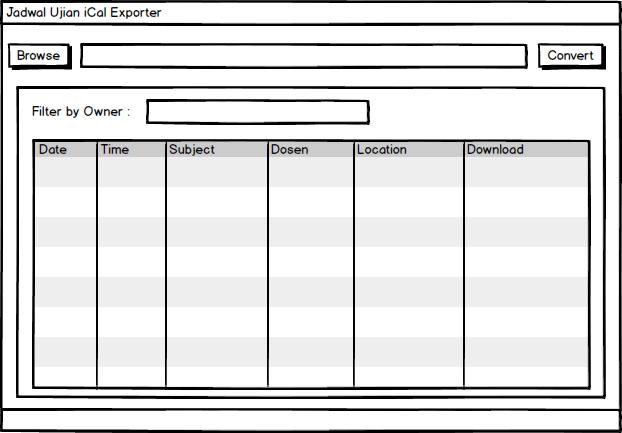
\includegraphics[scale=0.5]{Gambar/antarmuka}
		\caption{Tampilan awal Program}
		\label{fig:tampilan_awal}
		\end{figure}
		
		Pada gambar ~\ref{fig:tampilan_awal} terdapat beberapa \textit{button} dan \textit{textbox} yang memiliki fungsi sebagai berikut.
		\begin{itemize}
			\item \textit{}{Browse} : berfungsi untuk membuka \textit{pop-up window} sebagai sarana user memilih file excel yang akan dimasukan.
			\item \textit{Texbox path} : alamat file yang telah dipilih oleh user akan dicatat pada \textit{textbox} ini.
			\item \textit{Convert} : tombol ini berfungsi mengeksekusi program untuk membaca file yang telah dimasukan oleh user.
			\item \textit{Texbox filter} : merupakan fitur untuk memfilter jadwal mengawas berdasarkan nama dosen yang sesuai dengan \textit{input} user.
			\item \textit{TableView} : jadwal yang telah dibaca pada excel selanjutnya akan ditampilkan pada tabel ini. tabel ini terdiri dari kolom tanggal, waktu, matakuliah, dosen, lokasi, dan \textit{download} untuk mengunduh file iCal.		
		\end{itemize}
	\item Halaman untuk melakukan \textit{Browse} file excel\\
	Halaman ini merupakan halaman dimana user melakukan pemilihan input file excel jadwal mengawas. Halaman \textit{browser} menyesuaikan tipe sistem operasi yang dipakai.
		\begin{figure}[H]
		\centering
		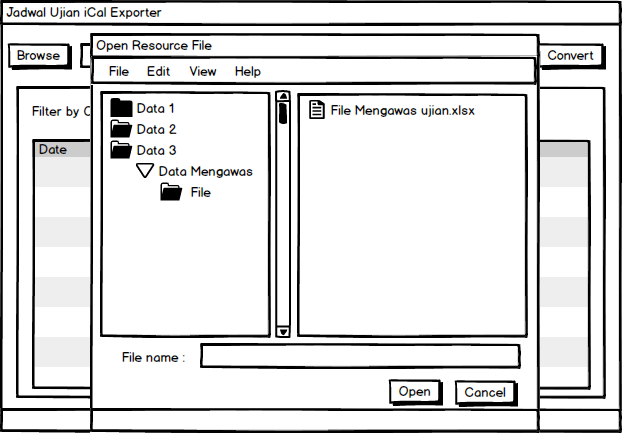
\includegraphics[scale=0.5]{Gambar/antarmuka3}
		\caption{Tampilan \textit{Browse} file excel}
		\label{fig:browse}
		\end{figure}
	\item Halaman setelah excel dibaca\\
	Halaman ini menujukan ketika file excel telah sukses dibaca dan ditampilkan pada \textit{tableview}.
		\begin{figure}[H]
		\centering
		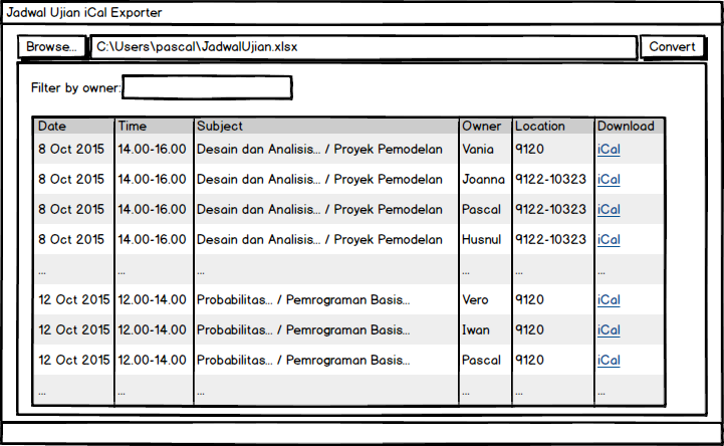
\includegraphics[scale=0.5]{Gambar/antarmuka2}
		\caption{Tampilan setelah excel dibaca}
		\label{fig:excel_dibaca}
		\end{figure}
	\item Halaman untuk menyimpan iCal\\
	Halaman ini dimana user telah memilih salah satu jadwal dan akan menyimpannya dalam betuk iCal. Halaman \textit{save} menyesuaikan sistem operasi yang dipakai. 
		\begin{figure}[H]
		\centering
		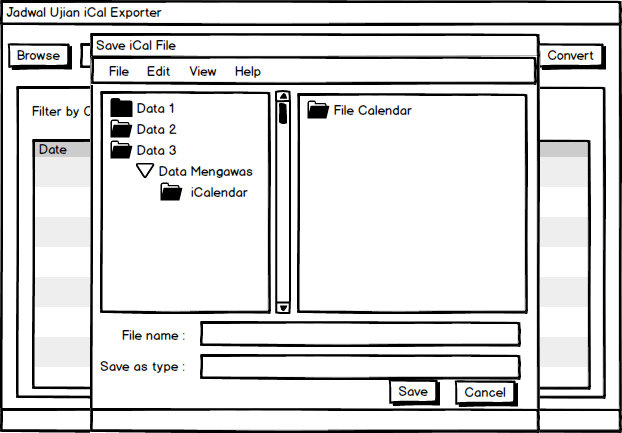
\includegraphics[scale=0.5]{Gambar/antarmuka4}
		\caption{Tampilan untuk menyimpan iCal}
		\label{fig:jadwalpng}
		\end{figure}
\end{enumerate}

\section{Rancangan \textit{Method-Method} Utama}
Berikut ini adalah rancangan \textit{method} utama program jadwal mengawas ujian yang akan dibangun perangkat lunaknya :
\begin{enumerate}
	\item Converter() - ExcelConverter\\
	\begin{tabular}{l c p{9cm}}
		Input & : & - \\ 
		Output & : & List<ScheduleClass>  \\ 
		Deskripsi & : & Method ini membaca excel yang di input oleh user dan mengkonversikannya kedalam bentuk list\\
		Algoritma & : & \begin{enumerate}
			\item Ambil path file yang telah di input oleh user
			\item Cari kolom No. pada file excel dan jadikan acuan bahwa program akan membaca setelah dari index kolom tersebut
			\item Baca baris per baris namun cek terlebih dahulu apakah di kolom No. baris tersebut masih berupa nomer, apabila tidak maka berhenti membaca karena baris yang berisi jadwal sudah terbaca semua
			\item Cek apakah baris mengandung kata \textit{LIBUR} bila iya maka lewati saja
			\item Pisahkan hari dan tanggal lalu konversi menjadi localDate. 
			\item Pisahkan jam menjadi jamAwal dan jamAkhir, lalu konversi menjadi localTime.
			\item jika menemukan kata \textit{Shift} atau \textit{Lab} maka lokasi ujian adalah Lab
			\item Masukan semua kedalam sebuah arrayList<ScheduleClass>
		\end{enumerate}
		\end{tabular}	
	
	\item Mergering() - ExcelConverter\\
	\begin{tabular}{l c p{9cm}}
		Input & : & List<ScheduleClass> \\ 
		Output & : & List<ScheduleClass> \\ 
		Deskripsi & : & Method ini mengatasi duplikat \textit{entry} dari dosen yang mempunyai dua jadwal mengawas pada hari yang sama\\
		Algoritma & : & 
			\begin{enumerate}
				\item Cari subject/mata kuliah yang tidak memiliki dosen pada arrayList yang telah di proses oleh \textit{method} Convert() karena bila program membaca kolom merger maka hanya kolom pertama saja yang dibaca sehingga kolom keduanya kosong.
				\item Masukan baris yang tidak memiliki dosen kedalam arrayList baru
				\item Hapus baris yang tidak memiliki dosen pada arrayList master
				\item Cocokan waktu dan tanggal ujian arrayList master dengan temp, bila sama maka tambahkan matakuliah/subject pada arrayList master
			\end{enumerate}
		\end{tabular}	
	
	\item calConverter() - CalendarConverter\\
	\begin{tabular}{l c p{9cm}}
		Input & : & sch: ScheduleClass , path: String\\ 
		Output & : & void \\ 
		Deskripsi & : & Method ini mengkonversi ScheduleClass menjadi iCal\\
		Algoritma & : & 
			\begin{enumerate}
				\item Inisiasi variable timezone Indonesia
				\item Konversi tanggal, bulan, dan tahun kedalam GregorianCalender
				\item Masukan event berdasarkan subject/mata kuliah , lokasi, dan dosen yang mengawas.
				\item Inisiasi kalender dan masukan variable tanggal dan event yang telah dibuat sebelumnya kedalam variable kalender tersebut
				\item Simpan pada path yang telah di pilih oleh user
			\end{enumerate}
		\end{tabular}	
		
	\item filterConvertion() - FXMLDocumentController\\
	\begin{tabular}{l c p{9cm}}
		Input & : & void\\ 
		Output & : & void \\ 
		Deskripsi & : & Method ini menjalankan filter data dosen sesuai input user\\
		Algoritma & : & 
			\begin{enumerate}
				\item Inisiasi tabel dengan list yang sudah di filter
				\item Masukan nilai yang sama kedalam list filter jika dosen yang dicari sesuai dengan input user.
				\item Atur kembali urutan tabel pada perangkat lunak
			\end{enumerate}
		\end{tabular}	
\end{enumerate}
}{}
\ifdefstring{\vbabe}{1}{\chapter{Implementasi dan Pengujian}
\label{chap:implementation}
Pada bagian ini akan dijelaskan mengenai lingkungan implementasi perangkat keras maupun perangkat lunak. Serta implementasi program iCalendar Converter beserta tampilan antar muka. Terakhir akan dibahas mengenai pengujian pada perangkat lunak ini.

\section{Implementasi}
Pada bab ini akan dijabarkan mengenai lingkungan pengembangan perangkat lunak disertai dengan pengujian.

\subsection{Lingkungan Implementasi}
Dalam mengimplementasikan program terdapat dua lingkungan pendukung, yaitu lingkungan perangkat keras dan lingkungan perangkat lunak.
\subsubsection{Lingkungan Perangkat Keras}
Dalam mengembangkan perangkat ini, digunakan spesifikasi perangkat keras sebagai berikut:
\begin{itemize}
	\item \textit{Processor} : Intel Core i7 2.4 Ghz
	\item \textit{Memory} : 8 GB
	\item \textit{Hardisk} : 640 GB
	\item VGA : Nvidia GeForce 540M
	\item \textit{keyboard} dan \textit{mouse standard}
\end{itemize}

\subsubsection{Lingkungan Perangkat Lunak}
Untuk pengembangan perangkat lunak iCalendar Converter, digunakan spesifikasi sebagai berikut:
\begin{itemize}
	\item IDE : Netbeans 8.1
	\item JDK : 1.8
	\item JRE : Java Runtime Enviroment 8
	\item Serta library pihak ketiga seperti JavaFX, Apache POI, dan iCal4j
	\item Editor antarmuka menggunakan SceneBuilder
\end{itemize}

\subsection{Implementasi Program}
Subbab ini menjelaskan tahap dimana program akan dibuat dan dikembangkan dari hasil analisis dan perancangan kelas-kelas maupun \textit{method} yang digunakan. Kode program lengkap dapat dilihat pada Lampiran A. 
Berikut ini merupakan penjelasan kode program dari perangkat lunak iCalendarConverter :
\begin{enumerate}
	\item Kode Program untuk menyimpan jadwal \\
	ScheduleClass merupakan kelas model yang ditujukan untuk menyimpan informasi jadwal yang telah dibaca.\\
	Baris (115-127) kelas ScheduleClass pada lampiran ~\ref{lst:ScheduleClass} menjelaskan tentang penggunaan StringProperty 
	dimana sebuah property memungkin untuk memberitahu jika ada perubahan pada variable tersebut. Property membantu untuk menjaga tampilan agar singkron dengan data. Pada ScheduleClass variable yang menggunakan StringProperty adalah dosen, subject, dan location.	
	\item Kode program untuk membaca Excel \\
	ExcelConverter merupakan kelas yang dikhususkan untuk membaca excel dan mengeluarkan \textit{output} berupa Arraylist dari kelas model ScheduleClass.\\
	Berikut ini merupakan urutan dari algoritma yang digunakan pada Excel Converter :
\begin{enumerate}
		\item Baris (68-84) pada lampiran ~\ref{lst:ExcelConverter} menjelaskan bagaimana program mencari kolom No. dan Nama Mata Kuliah pada excel, sebagai acuan bahwa setelah kolom itu merupakan data jadwal yang akan dibaca oleh program. Setelah diketahui dimana kolom No. dan Nama Kuliah berada, nomer baris dan kolomnya akan dimasukan kedalam variable sebagai acuan membaca program dimulai pada baris itu. Pemilihan kolom No. sebagai acuan karena isi kolom No. menandakan berapa banyak data jadwal yang ada, sehingga bila isi dari kolom No. bukan angka maka program akan berhenti membaca. Selanjutnya, pemilihan Nama Mata Kuliah sebagai acuan selain karena data pada kolom itu akan dimasukan ke kelas model, pun juga karena setelah kolom tersebut terdapat kolom ruang kuliah yang akan dimasukan kedalam variable lokasi pada program.
		Selain itu, nomer kolom ruangan dapat menjadi acuan lokasi dosen mengawas.
		\item Baris (85-87) pada lampiran ~\ref{lst:ExcelConverter} menjelaskan bahwa i sebagai acuan program membaca baris, sedangkan j sebagai acuan program membaca kolom.
		\item Baris (89-93) pada lampiran ~\ref{lst:ExcelConverter} menjelaskan bahwa bila baris ke i program membaca dan isinya kosong maka berhenti membaca.
		\item Baris (96-100) pada lampiran ~\ref{lst:ExcelConverter} menjelaskan bila isi pada kolom No. bukanlah angka dan \textit{blank} maka program berhenti membaca.
		\item Baris (101-107) pada lampiran ~\ref{lst:ExcelConverter} menjelaskan	bila isi kolom No. adalah kosong maka lewati barisnya dan baca baris selanjutnya.
		\item Baris (108-129) pada lampiran ~\ref{lst:ExcelConverter} menjelaskan bahwa bila kolom tersebut tanggal maka, jika isinya kosong maka lewati barisnya, jika tidak kosong maka pisahkan isinya menurut tanda - dan tanda , . Lalu, jika ada singkatan Mrt ganti menjadi 3, jika ada singktan Okt ganti menjadi 10 dan jika ada singkatan 16 maka ganti menjadi 2016. Sehingga format tanggal menjadi 2016-03-01 sebagai contoh. Setelah itu masukan ke variable LocalDate.
		\item Baris (130-163) pada lampiran ~\ref{lst:ExcelConverter} menjelaskan bahwa bila kolom tersebut adalah jam maka, jika isinya LIBUR maka lewati baris tersebut, jika isinya Shift maka pasti baris dibawahnya adalah jam, sehingga ambil value baris dibawahnya lalu pisahkan menurut tanda - dan ganti tanda . dengan tanda : . Lalu, masukan ke variable LocalTime. Jika isi kolom berisi jam saja, maka pisahkan menurut tanda - dan ganti tanda . dengan tanda : . Lalu, masukan ke variable LocalTime.
		\item Baris (164-166) pada lampiran ~\ref{lst:ExcelConverter} menjelaskan bila kolom tersebut adalah Nama Mata Kuliah maka masukan ke variable String Subject.
		\item Baris (173-192) pada lampiran ~\ref{lst:ExcelConverter} menjelaskan bila kolom tersebut adalah ruangan yang bearti isinya adalah nama dosen yang mengawas maka, jika isi kolom diawali dengan Lab maka pisahkan menurut tanda : dan pisahkan kembali menurut tanda , sehingga menghasilkan nama dosen saja. Selanjutnya, masukan nama dosen ke ArrayList dosen dan isi ArrayList location dengan kata Lab. Jika isi kolom tidak di awali dengan kata lab maka masukan nama dosen ke ArrayList dosen dan isi ArrayList location dengan mengambil nomor kolom dari ruangan tersebut dan mencocokannya dengan posisi nama dosen tersebut berada dan isi nomer ruangan kedalam ArrayList Location.
		\item Baris (193-215) pada lampiran ~\ref{lst:ExcelConverter} menjelaskan bahwa karena dua mata kuliah berisikan dua baris kolom dosen yang di \textit{merger} jadi satu dan Apache POI hanya dapat membaca baris pertama kolom yang dimerger maka pada baris ini ArrayList dosen dan location disi dengan String kosong.
		\item Baris (219-221) pada lampiran ~\ref{lst:ExcelConverter} menjelaskan masukan semua variable yang diisi kedalam ArrayList ScheduleClass sesuai jumlah ArrayList nama dosen.
		\item Baris (222-223) pada lampiran ~\ref{lst:ExcelConverter} menjelaskan hapus semua isi ArrayList dosen agar tidak ada duplikasi.
		\item Baris (227) pada lampiran ~\ref{lst:ExcelConverter} menjelaskan hasil ArrayList method Converter() akan kembali dicek oleh method mergering().
		\item Baris (235-242) pada lampiran ~\ref{lst:ExcelConverter} menjelaskan jika ada dosen yang isinya kosong pada ArrayList ScheduleList maka pindahkan isinya ke ArrayList baru yang bernama ScheduleListSmt. Hal ini karena dua matakuliah yang berbeda di awas oleh satu dosen dan sehingga nantinya subject yang variable dosennya kosong akan dipindahkan ke variable dosen yang ada nama dosennya.
		\item Baris (243-250) pada lampiran ~\ref{lst:ExcelConverter} menjelaskan hapus isi ArrayList ScheduleList yang sama dengan ArrayList SchedulelistSmt.
		\item Baris (251-263) pada lampiran ~\ref{lst:ExcelConverter} menjelaskan jika tanggal dan jam pada ArrayList ScheduleList sama dengan ArrayList ScheduleListSmt maka tambahkan subject dari ArrayList ScheduleList dengan subject yang ada di ArrayList ScheduleListSmt.
		\item Baris (264) pada lampiran ~\ref{lst:ExcelConverter} menjelaskan kembalian ArrayList ScheduleList.				
	\end{enumerate}

\item Kode Program untuk Konversi Kalendar \\
Kelas CalendarConverter merupakan kelas yang dikhususkan untuk mengkonversi ScheduleClass menjadi file iCalendar. \\
Berikut ini penjelasan dari implementasi kelas CalendarConverter :
\begin{enumerate}
	\item Baris (41-43) pada lampiran ~\ref{lst:CalendarConverter} menjelaskan pembuatan timeZone untuk wilayah Indonesia.
	\item Baris (46-52) pada lampiran ~\ref{lst:CalendarConverter} menjelaskan pembuatan tanggal dan waktu dimulainya ujian dengan mengkonversi tahun, bulan, tanggal, jam, dan menit dari ScheduleClass.
	\item Baris (55-61) pada lampiran ~\ref{lst:CalendarConverter} menjelaskan pembuatan tanggal dan waktu ujian tersebut berakhir dengan mengkonversi tahun, bulan, tanggal, jam, dan menit dari ScheduleClass.
	\item Baris (65-72) pada lampiran ~\ref{lst:CalendarConverter} menjelaskan pembuatan event pada kalendar.
	\item Baris (80) pada lampiran ~\ref{lst:CalendarConverter} memasukan timeZone pada kalendar.
	\item Baris (83-85) pada lampiran ~\ref{lst:CalendarConverter} menjelaskan pembuat identitas pembuat calendar.
	\item Baris (89-92) pada lampiran ~\ref{lst:CalendarConverter} menjelaskan cara pembuatan calendar.
	\item Baris (95-96) pada lampiran ~\ref{lst:CalendarConverter} memasukan event yang telah dibuat kedalam kalendar dan print sesudahnya.
	\item Baris (99-105) pada lampiran ~\ref{lst:CalendarConverter} menjelaskan cara menyimpan file iCalendar pada direktori tertentu.
\end{enumerate}

\item Kode Program \textit{Controller} \\
Kelas FXMLDocumentController merupakan kelas yang bertugas menjadi penghubung kelas \textit{view} dengan kelas-kelas lainnya. Di kelas ini hasil dari excel yang telah dibaca akan ditampilkan pada tabelview dan semua fungsi \textit{button} dan  \textit{textbox} di atur dalam kelas ini. \\
Berikut ini penjelasan dari kode-kode dalam kelas FXMLDocumentController :
\begin{enumerate}
	\item Baris (55-58) pada lampiran ~\ref{lst:FXMLDocumentController} menjelaskan file yang akan dipilih nanti harus berekstensi .xls atau .xlsx.
	\item Baris (59) pada lampiran ~\ref{lst:FXMLDocumentController} menjelaskan bagaimana memunculkan \textit{pop-up window} untuk memilih file input.
	\item Baris (61-68) pada lampiran ~\ref{lst:FXMLDocumentController} menjelaskan jika file tidak kosong maka ambil \textit{path}file tersebut dan isikan \textit{textbox browse} dengan \textit{path} tersebut.
	\item Baris (74-75) pada lampiran ~\ref{lst:FXMLDocumentController} menjelaskan konversi file excel tersebut, kemudian ambil hasilnya dan masukan kedalam ObservableArrayList.
	\item Baris (78-84) pada lampiran ~\ref{lst:FXMLDocumentController} menjelaskan cara menampilkan hasil konversi kedalam \textit{tableview} dengan mengisikan sesuai urutan kolom pada \textit{tableview}.
	\item Baris (86-95) pada lampiran ~\ref{lst:FXMLDocumentController} menjelaskan masukan semua ObservableArrayList jadwalList kedalam ObservableArrayList filteredData untuk keperluan filter nanti dan jika ada perubahan pada ObservableArrayList jadwalList maka \textit{update} pula ObservableArrayList filteredData.
	\item Baris (108) pada lampiran ~\ref{lst:FXMLDocumentController} menjelaskan ambil kelas ScheduleClass yang dipilih oleh user dan masukan kedalm variable selected.
	\item Baris (111-112) pada lampiran ~\ref{lst:FXMLDocumentController} menjelaskan bahwa setiap file yang akan disimpan diberikan ekstensi .ics .
	\item Baris (113) pada lampiran ~\ref{lst:FXMLDocumentController} menjelaskan cara memunculkan \textit{save dialog}.
	\item Baris (117-126) pada lampiran ~\ref{lst:FXMLDocumentController} menjelaskan ambil path direktori dimana user akan menyimpan file, lalu konversi jadwal yang telah dipilih oleh user dan simpan di direktori yang sudah ditentukan.
	\item Baris (131-140) pada lampiran ~\ref{lst:FXMLDocumentController} menjelaskan jika \textit{textbox filter} di isi oleh user maka jadwal di tabel pun berubah sesuai dengan nama dosen yang di tuliskan user.
	\item Baris (145-154) pada lampiran ~\ref{lst:FXMLDocumentController} menjelaskan cara \textit{update} filteredData sesuai nama dosen yang di input oleh user.
	\item Baris (158-170) pada lampiran ~\ref{lst:FXMLDocumentController} menjelaskan
\end{enumerate}
	
\end{enumerate}

\section{Implementasi Antarmuka}
Berikut ini implementasi antarmuka dari perangkat lunak iCalendarConverter :
\begin{enumerate}
	\item Tampilan perangkat lunak iCalendarConverter
		\begin{figure}[H]
		\centering
		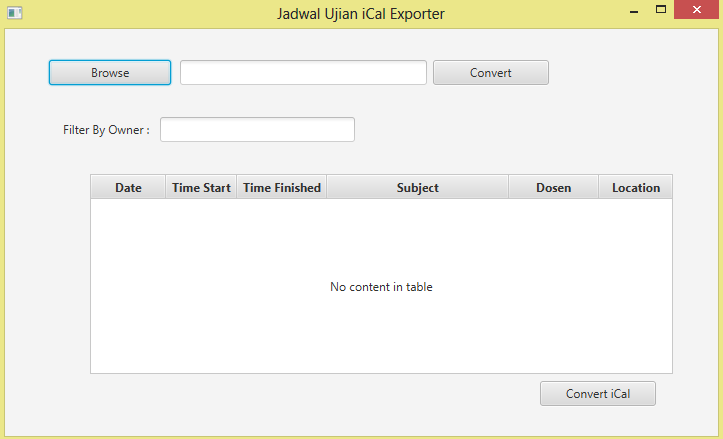
\includegraphics[scale=0.7]{Gambar/implementAntarmuka}
		\caption{Tampilan antarmuka perangkat lunak}
		\label{fig:implementAntarmuka}
		\end{figure}
	\item Tampilan Antarmuka ketika file excel jadwal mengawas telah dimasukan
		\begin{figure}[H]
		\centering
		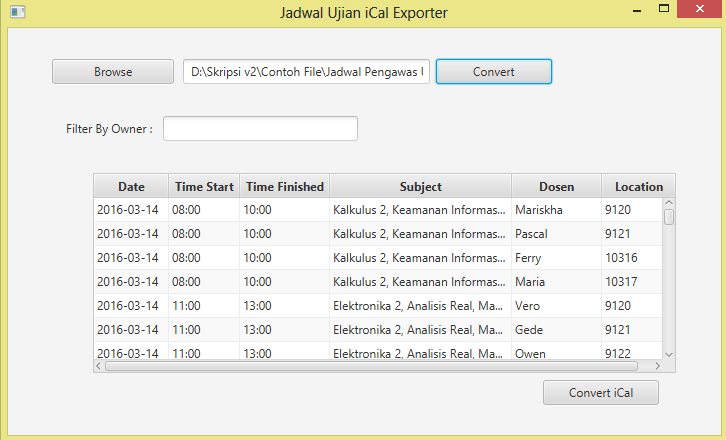
\includegraphics[scale=0.7]{Gambar/implementAntarmuka2}
		\caption{Tampilan antarmuka setelah file mengawas dimasukan}
		\label{fig:implementAntarmuka}
		\end{figure}
\end{enumerate}

\section{Pengujian}
Pada subbab ini akan dilakukan pengujian pada perangkat lunak untuk mengetahui apakah program dapat berjalan sesuai dengan apa yang di inginkan. Terdapat dua pengujian yaitu :
\begin{enumerate}
	\item Pengujian Fungsional.
	\item Pengujian Eksperimental.
\end{enumerate}

\subsection{Pengujian Fungsional}
Pada pengujian ini akan di uji mengenai fungsionalitas dari perangkat lunak ini, Berikut hasil pengujiannya : 
\begin{table}[H]
	\centering
		\caption{Tabel hasil pengujian fungsional}
		\label{tab:fungsional}
		\begin{tabular}{ | p{4cm} | p{4cm} | p{4cm} | c |}
			\hline
				Hal yang diuji & Hasil yang diharapkan & Hasil Pengujian & Status \\ \hline
				Browse file Excel & PL dapat melakukan browse file excel & PL dapat melakukan browse file excel & OK \\ \hline
				Path File Excel & PL dapat menangkap path file dari input & PL dapat menangkap path file dari input & OK \\ \hline
				Menampilkan Jadwal ke layar & PL menampilkan ke layar file excel yang telah dibaca  & PL menampilkan ke layar file excel yang telah dibaca & OK \\ \hline
				Konversi ke iCal & PL dapat mengkonversi jadwal kedalam iCalendar & PL dapat mengkonversi jadwal kedalam iCalendar & OK \\ \hline
				Filter nama dosen & PL dapat menampilkan nama dosen yang telah di filter & PL dapat menampilkan nama dosen yang telah di filter & OK \\ \hline
				Hasil Filter dapat dikonversi ke iCal & Hasil Filter pada PL dapat di konversikan kedalam iCal & Hasil Filter pada PL dapat di konversikan kedalam iCal & OK \\ \hline
				Import Google Calendar & Hasil konversi PL dapat di masukan kedalam Google Calendar & Hasil konversi PL dapat di masukan kedalam Google Calendar & OK \\ \hline
				Dapat dibuka di Outlook & Hasil konversi PL dapat di buka di Outlook & Hasil konversi PL dapat di buka di Outlook & OK \\ \hline
				Hasil filter dapat di import Google Calendar & Hasil filter konversi PL dapat di masukan kedalam Google Calendar & Hasil filter konversi PL dapat di masukan kedalam Google Calendar & OK \\ \hline
				Hasil filter Dapat dibuka di Outlook & Hasil filter konversi PL dapat di buka di Outlook & Hasil filter konversi PL dapat di buka di Outlook & OK \\ \hline
		\end{tabular}
\end{table}

Berikut ini adalah tampilan dari hasil pengujian yang telah dilakukan pada tabel ~\ref{tab:fungsional} :
\begin{enumerate}
	\item Browse File
		\begin{figure}[H]
		\centering
		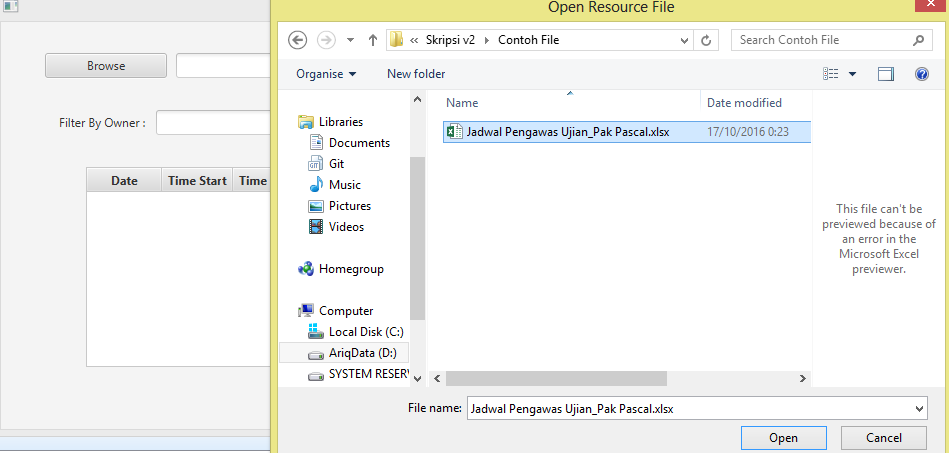
\includegraphics[scale=0.7]{Gambar/browseFile}
		\caption{Tampilan browse file excel mengawas ujian}
		\label{fig:browseFile}
		\end{figure}
	\item Path File Excel
		\begin{figure}[H]
		\centering
		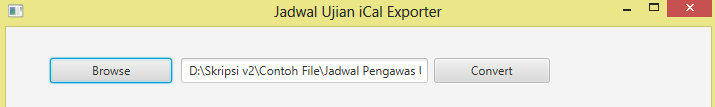
\includegraphics[scale=0.7]{Gambar/pathFile}
		\caption{Tampilan path file excel mengawas ujian}
		\label{fig:pathFile}
		\end{figure}
	\item Menampilkan jadwal ke layar
		\begin{figure}[H]
		\centering
		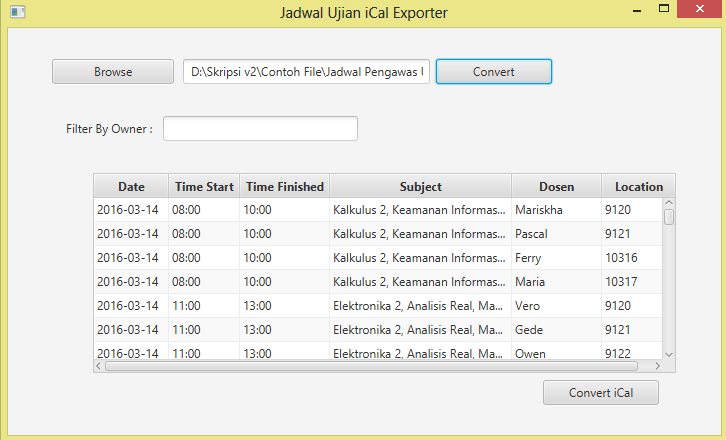
\includegraphics[scale=0.7]{Gambar/implementAntarmuka2}
		\caption{PL menampilkan jadwal ke layar}
		\label{fig:jadwalKeLayar}
		\end{figure}
	\item Konversi ke iCal
		\begin{figure}[H]
		\centering
		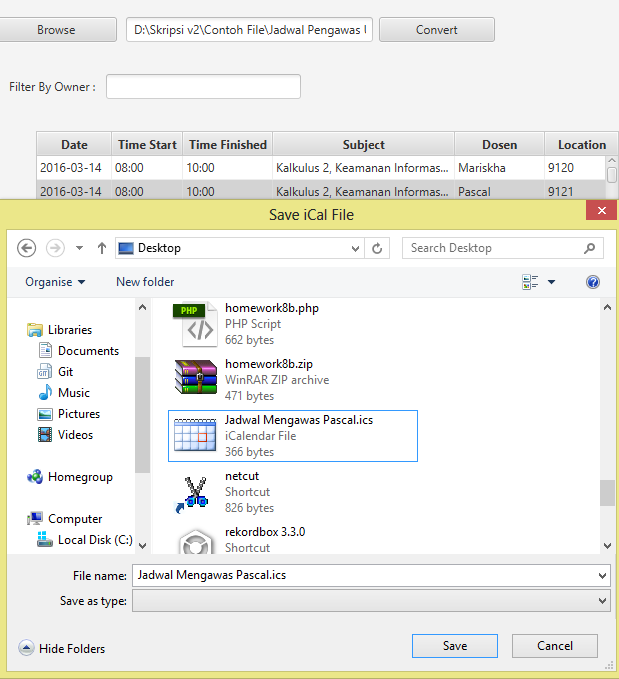
\includegraphics[scale=0.5]{Gambar/konversiiCal}
		\caption{PL mengkonversi jadwal ke format iCal}
		\label{fig:konversiiCal}
		\end{figure}
		
		\begin{figure}[H]
		\centering
		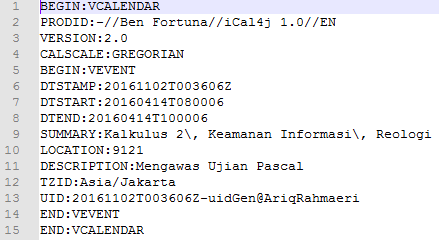
\includegraphics[scale=0.7]{Gambar/fileiCal}
		\caption{File iCal}
		\label{fig:fileiCal}
		\end{figure}
	\item Filter nama dosen
		\begin{figure}[H]
		\centering
		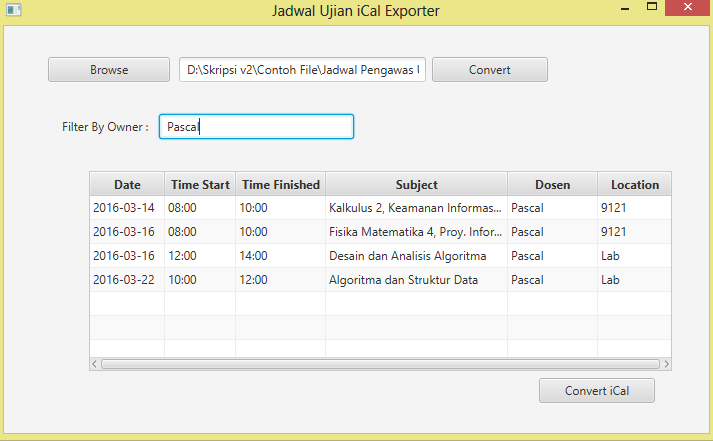
\includegraphics[scale=0.7]{Gambar/filterDosen}
		\caption{Hasil pengujian filter nama dosen}
		\label{fig:filterDosen}
		\end{figure}
	\item Convert hasil filter kedalam iCal
		\begin{figure}[H]
		\centering
		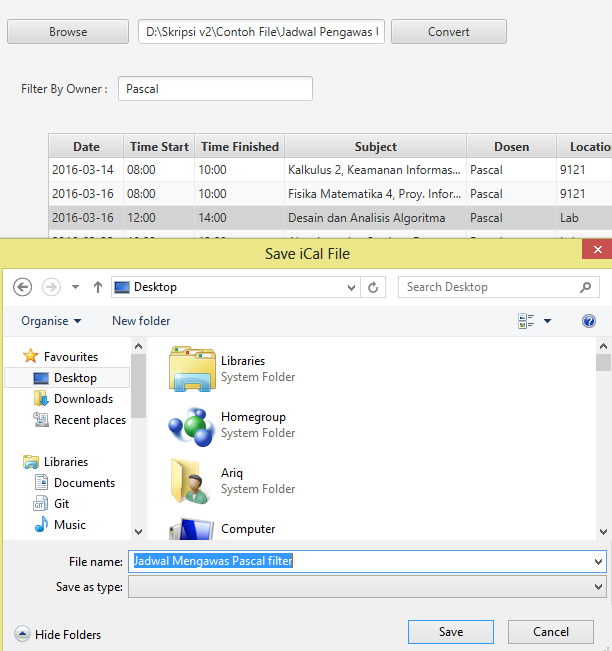
\includegraphics[scale=0.5]{Gambar/filterKonvertiCal}
		\caption{Hasil pengujian convert hasil filter kedalam iCal}
		\label{fig:filterKonvertiCal}
		\end{figure}
		
		\begin{figure}[H]
		\centering
		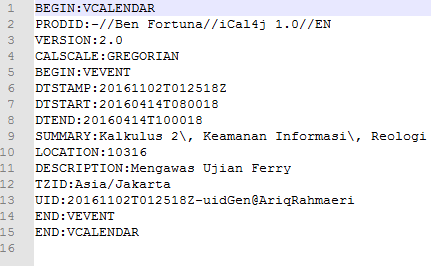
\includegraphics[scale=0.5]{Gambar/fileiCalFilter}
		\caption{File iCal Filter}
		\label{fig:fileiCalFilter}
		\end{figure}
	
	\item Import Google Calendar
		\begin{figure}[H]
		\centering
		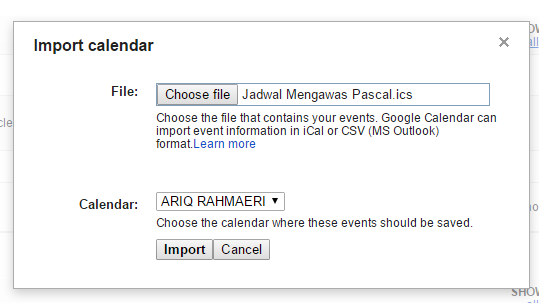
\includegraphics[scale=0.7]{Gambar/importGC}
		\caption{Hasil pengujian import kedalam Google Calendar}
		\label{fig:importGC}
		\end{figure}
		
		\begin{figure}[H]
		\centering
		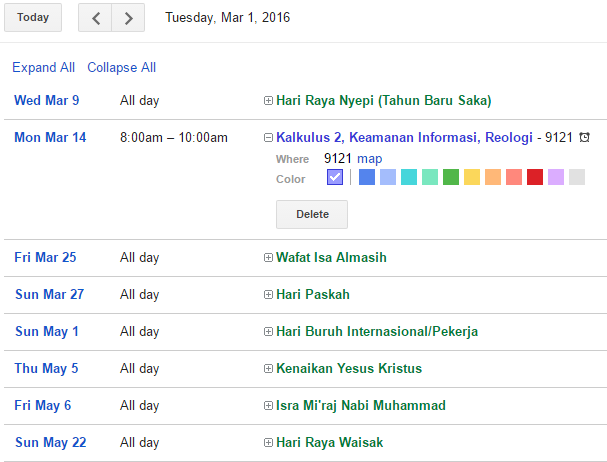
\includegraphics[scale=0.7]{Gambar/hasilGC}
		\caption{Hasil import ke Google Calendar}
		\label{fig:hasilGC}
		\end{figure}
		
		\begin{figure}[H]
		\centering
		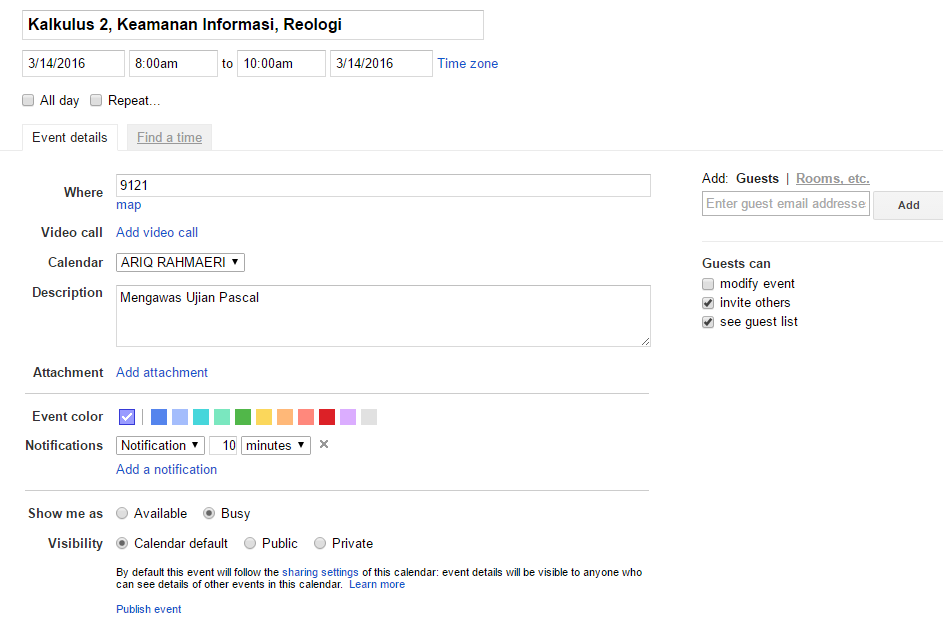
\includegraphics[scale=0.5]{Gambar/hasilGC2}
		\caption{Hasil import ke Google Calendar bagian 2 }
		\label{fig:hasilGC2}
		\end{figure}
		
		\item Buka di MS Outlook
			\begin{figure}[H]
			\centering
			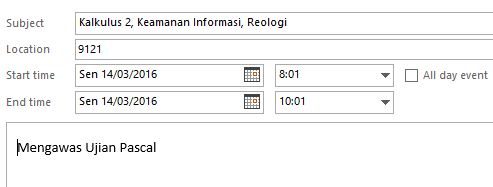
\includegraphics[scale=0.7]{Gambar/hasilOutlook}
			\caption{File hasil Konversi dapat dibuka di MS Outlook }
			\label{fig:hasilOutlook}
			\end{figure}
		
		\item Import hasil filter kedalam Google Calendar
			\begin{figure}[H]
			\centering
			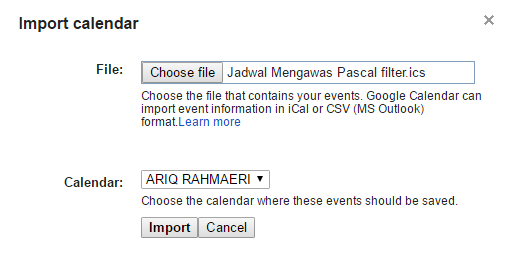
\includegraphics[scale=0.7]{Gambar/importGCFilter}
			\caption{Hasil pengujian import file yang di filter kedalam Google Calendar }
			\label{fig:importGCFilter}
			\end{figure}
			
			\begin{figure}[H]
			\centering
			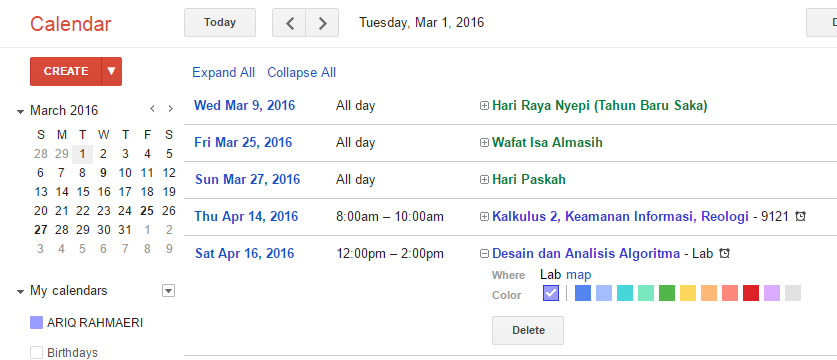
\includegraphics[scale=0.7]{Gambar/hasilGCFilter}
			\caption{Hasil import file yang di filter ke Google Calendar}
			\label{fig:hasilGCFilter}
			\end{figure}
			
			\begin{figure}[H]
			\centering
			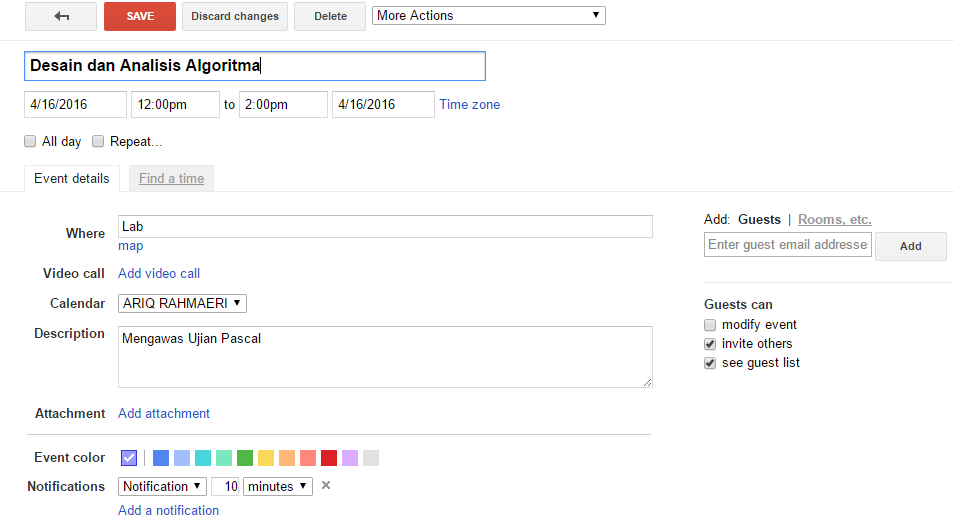
\includegraphics[scale=0.5]{Gambar/hasilGCFilter2}
			\caption{Hasil import file yang di filter ke Google Calendar bagian 2 }
			\label{fig:hasilGCFilter2}
			\end{figure}
			
		\item Buka hasil filter di MS Outlook
			\begin{figure}[H]
			\centering
			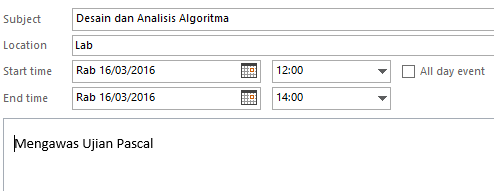
\includegraphics[scale=0.7]{Gambar/hasilOutlookFilter}
			\caption{File hasil filter dapat dibuka di MS Outlook }
			\label{fig:hasilOutlookFilter}
			\end{figure}
			
		
\end{enumerate} 

}{}
\ifdefstring{\vbabf}{1}{\chapter{Kesimpulan}
\label{chap:summary}

Kesimpulan dari pembangunan perangkat lunak ini adalah bahwa jadwal mengawas ujian yang dikeluarkan oleh TU dapat digunakan sebagai input PL untuk ditampilkan ke layar dan dikonversikan menjadi iCal. Dengan adanya iCal jadwal mengawas ujian yang dikeluarkan oleh TU tidak perlu dicetak dan dibagikan kepada dosen satu persatu. Cukup dengan memasukannya pada PL dan mengintegrasikannya pada \textit{platform} aplikasi yang mendukung iCalendar sehingga jadwal dapat dengan mudah di lihat pada \textit{smartphone} maupun perangkat lainnya yang terintegrasi dengan aplikasi iCalendar tersebut. Cara pembacaan file excel mengawas pada penelitian ini belum bisa dibilang yang paling efektif dan efisien. Pengembangan lebih lanjut sangat memungkinkan untuk memperkaya fitur-fitur yang ada pada perangkat lunak ini, sehingga semakin memudahkan dosen untuk mendapatkan jadwal mengawas ujian.  }{}
\ifdefstring{\vbabg}{1}{\include{Bab/bab7}}{}
\ifdefstring{\vbabh}{1}{\include{Bab/bab8}}{}
\ifdefstring{\vbabi}{1}{\include{Bab/bab9}}{}

\bibliographystyle{ieeetr}
\bibliography{pustaka}

\appendix
\apptoc

\tampillmp{\vlmp}
\ifdefstring{\vlmpa}{1}{\chapter{The Program}
\label{app:A}

The interface of the program is shown in Figure~\ref{fig:appxa2}:

\begin{figure}[H]
\centering
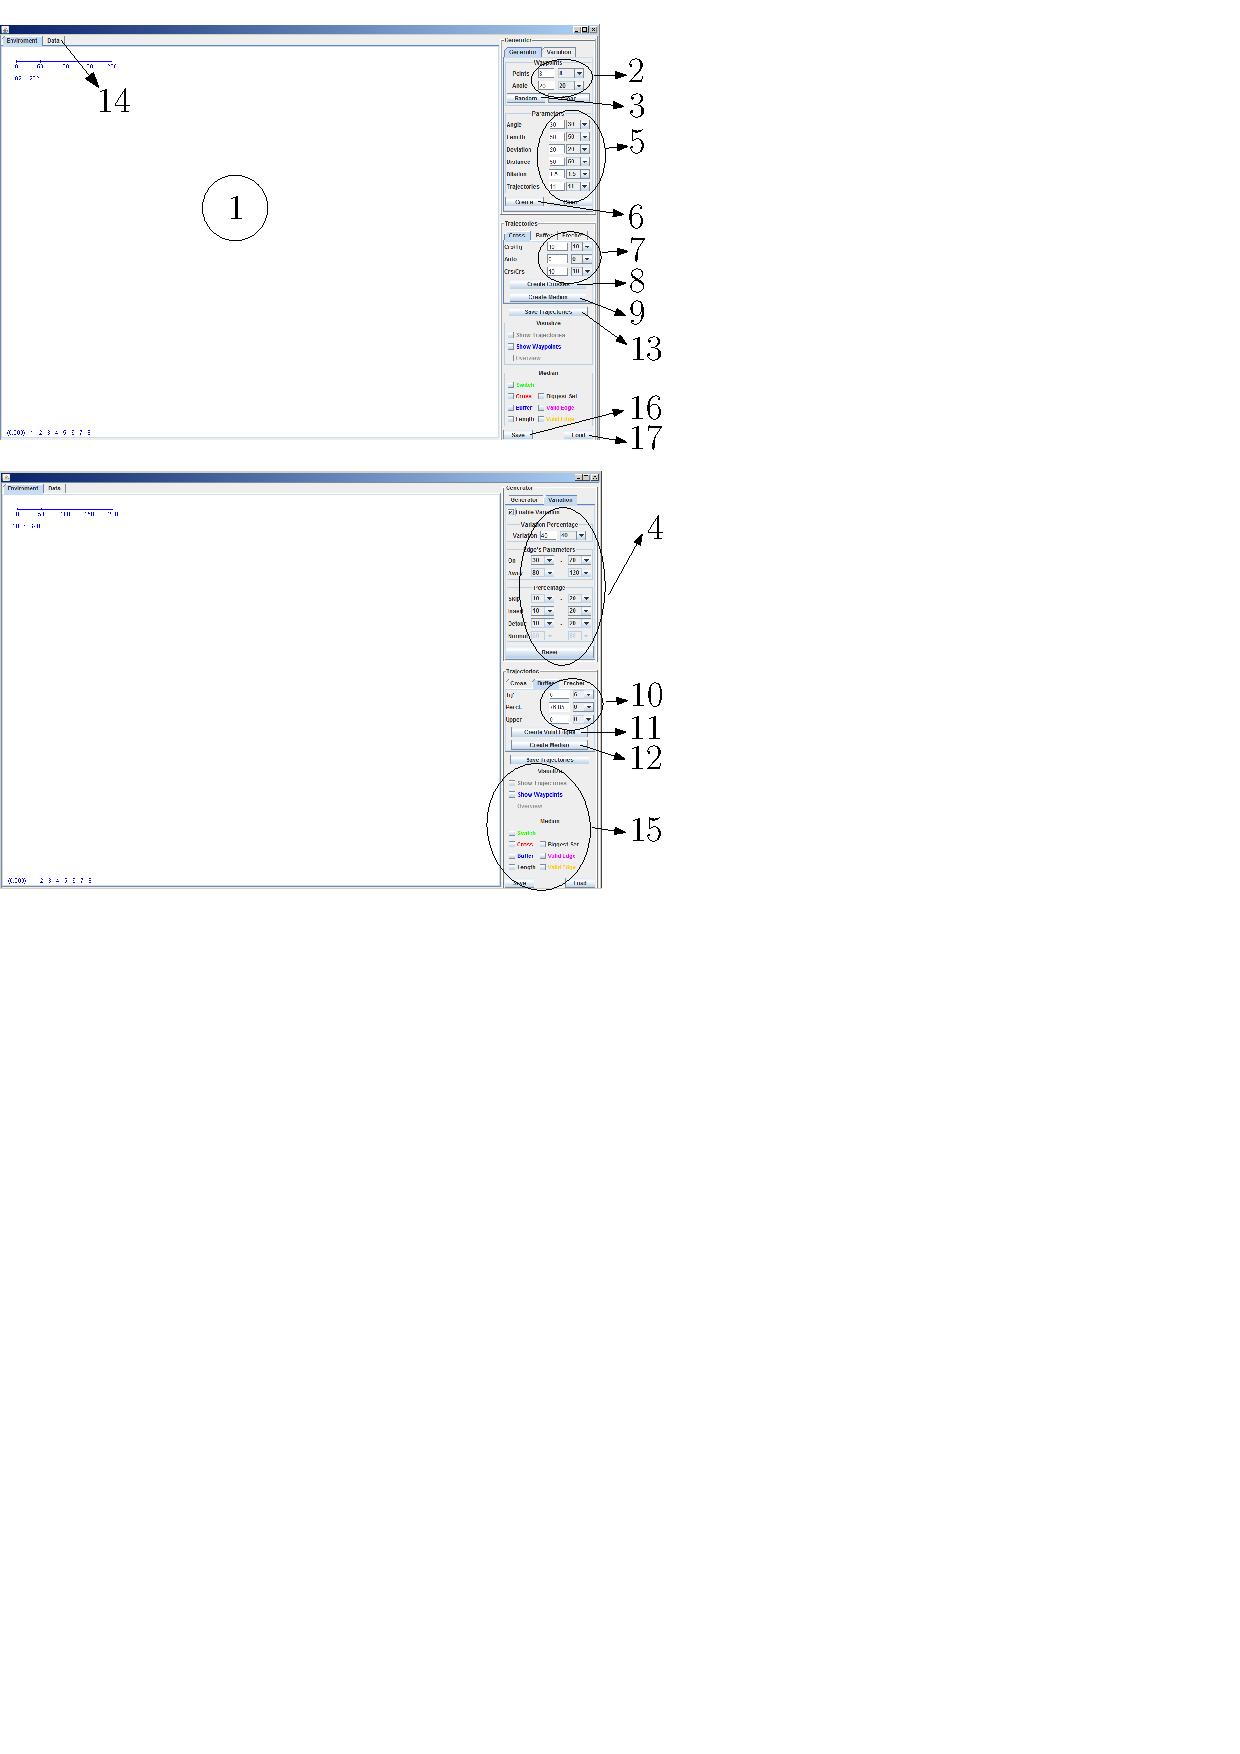
\includegraphics[scale=1]{Gambar/appxa2}
\caption[Interface of the program]{Interface of the program} 
\label{fig:appxa2}
\end{figure}

Step by step to compute the median trajectory using the program:
\begin{enumerate}
\item
Create several waypoints. 
Click anywhere in the ``Environment'' area(1) or create them automatically by setting the parameters for waypoint(2) or clicking the button ``Random''(3).
\item
The ``Variation'' tab could be used to create variations by providing values needed to make them(4).
\item
Create a set of trajectories by setting all parameters(5) and clicking the button ``Create''(6).
\item
Compute the median using the homotopic algorithm: 
\begin{itemize}
\item Define all parameters needed for the homotopic algorithm(7).
\item Create crosses by clicking the ``Create Crosses'' button(8).\item Compute the median by clicking the ``Compute Median'' button(9).
\end{itemize}
\item
Compute the median using the switching method and the buffer algorithm: 
\begin{itemize}
\item Define all parameters needed for the buffer algorithm(10).
\item Create valid edges by clicking the ``Create Valid Edges''button(11). 
\item Compute the median by clicking the ``Compute Median''button(12).
\end{itemize}
\item
Save the resulting median by clicking the ``Save Trajectories'' button(13).
The result is saved in the computer memory and can be seen in ``Data'' tab(14) 
\item 
The set of trajectories and its median trajectories will appear in the ``Environment'' area(1) and the user can change what to display by selecting various choices in ``Visualize'' and ``Median'' area(15).
\item
To save all data to the disk, click the ``Save''(16) button. A file dialog menu will appear.
\item
To load data from the disk, click the ``Load''(17) button.
\end{enumerate}}{}
\ifdefstring{\vlmpb}{1}{%versi 2 (8-10-2016)
\chapter{File Excel}
\label{lamp:B}

\begin{figure}[H]
		\centering
		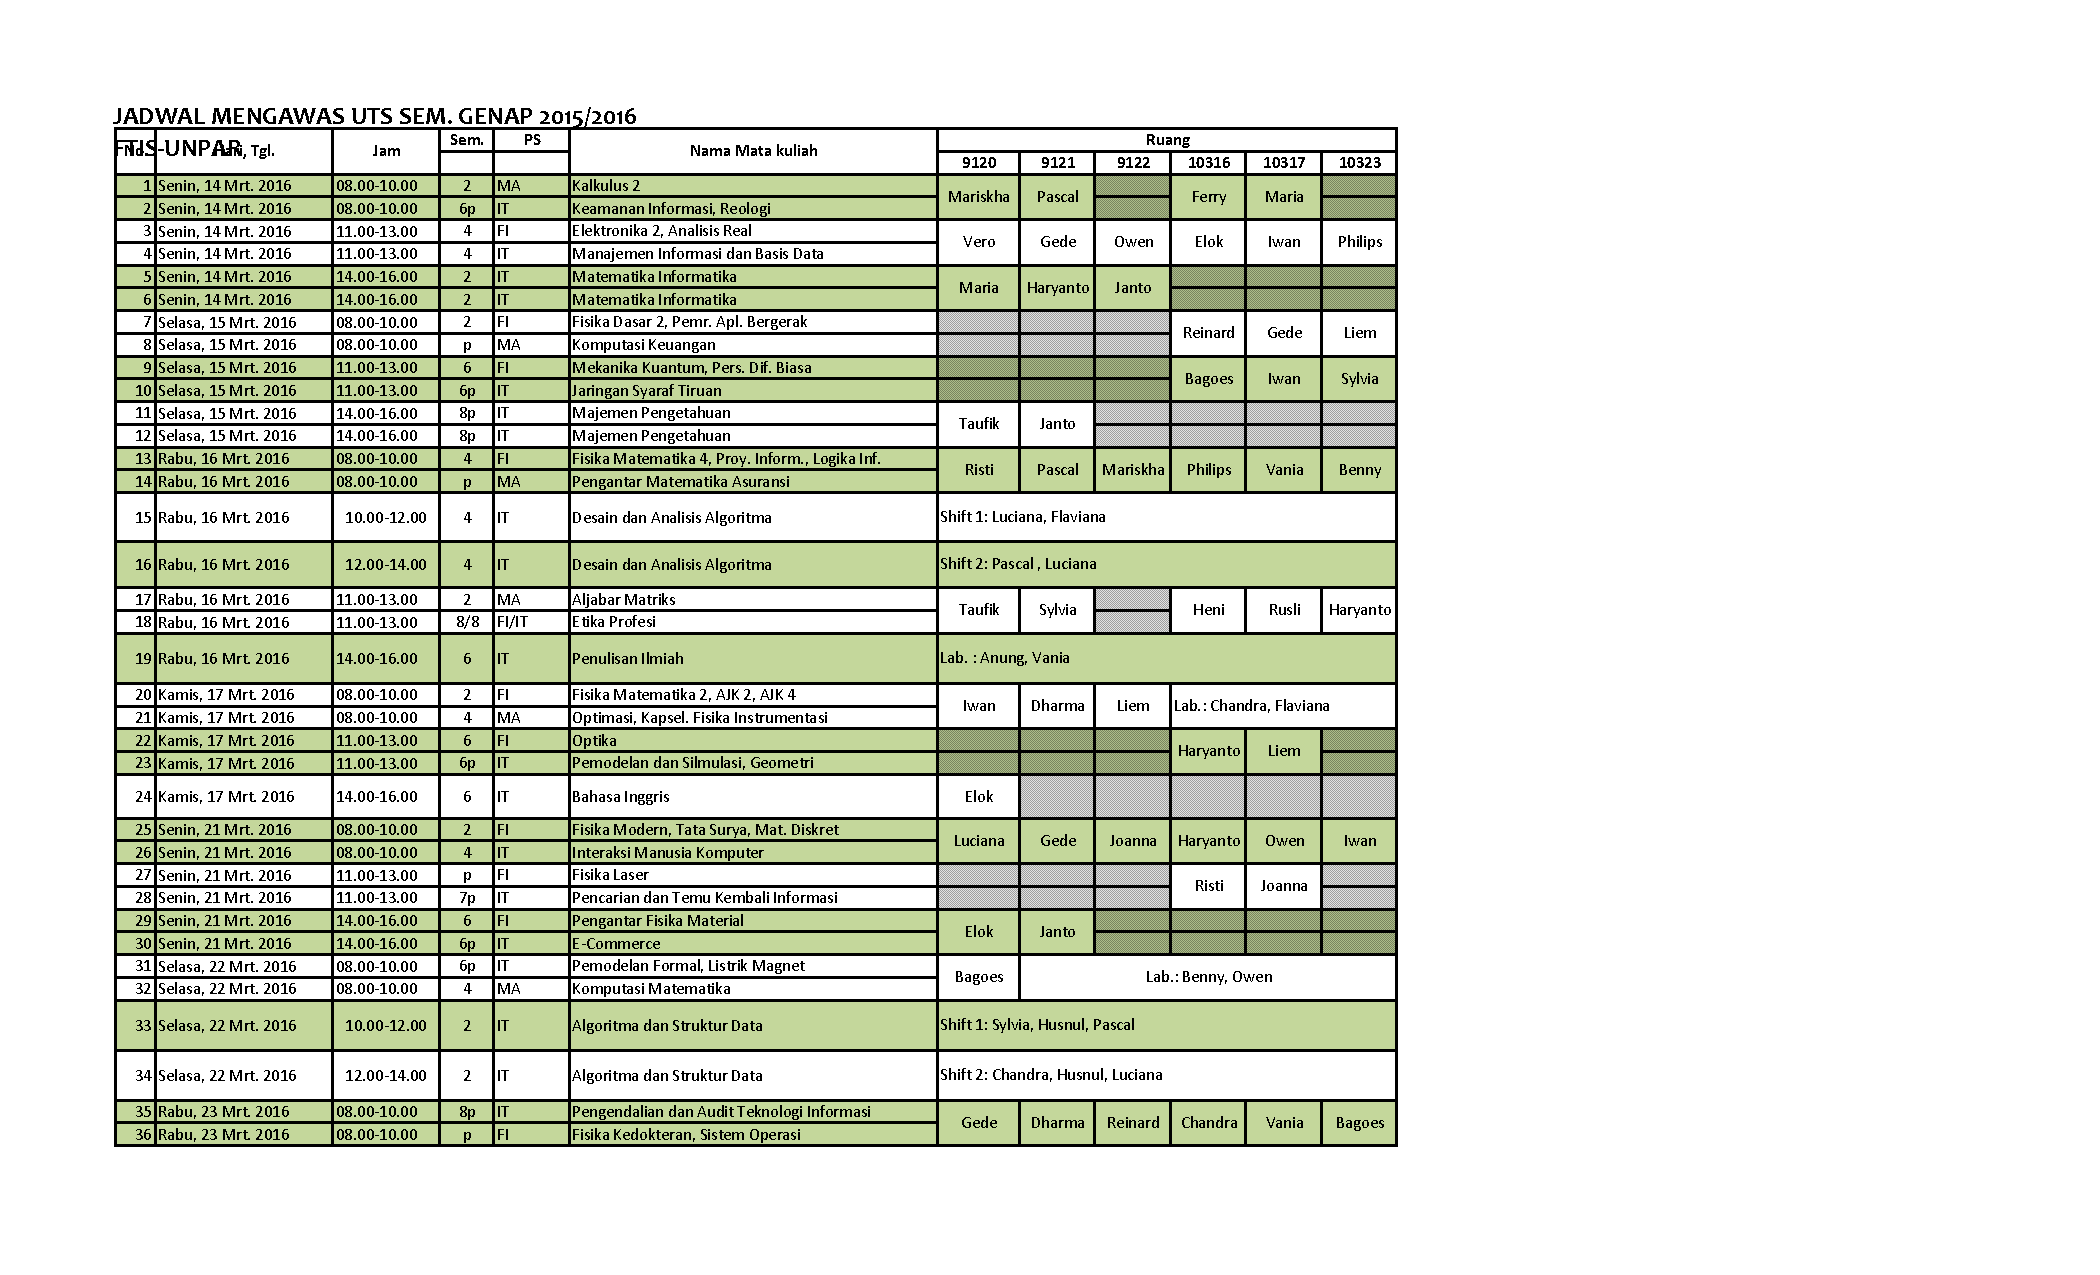
\includegraphics[scale=0.7]{Gambar/JadwalPengawasUjianPakPascal}
		\caption{File Excel Jadwal Mengawas Format Lama}
		\label{fig:formatLama}
\end{figure}

\begin{figure}[H]
		\centering
		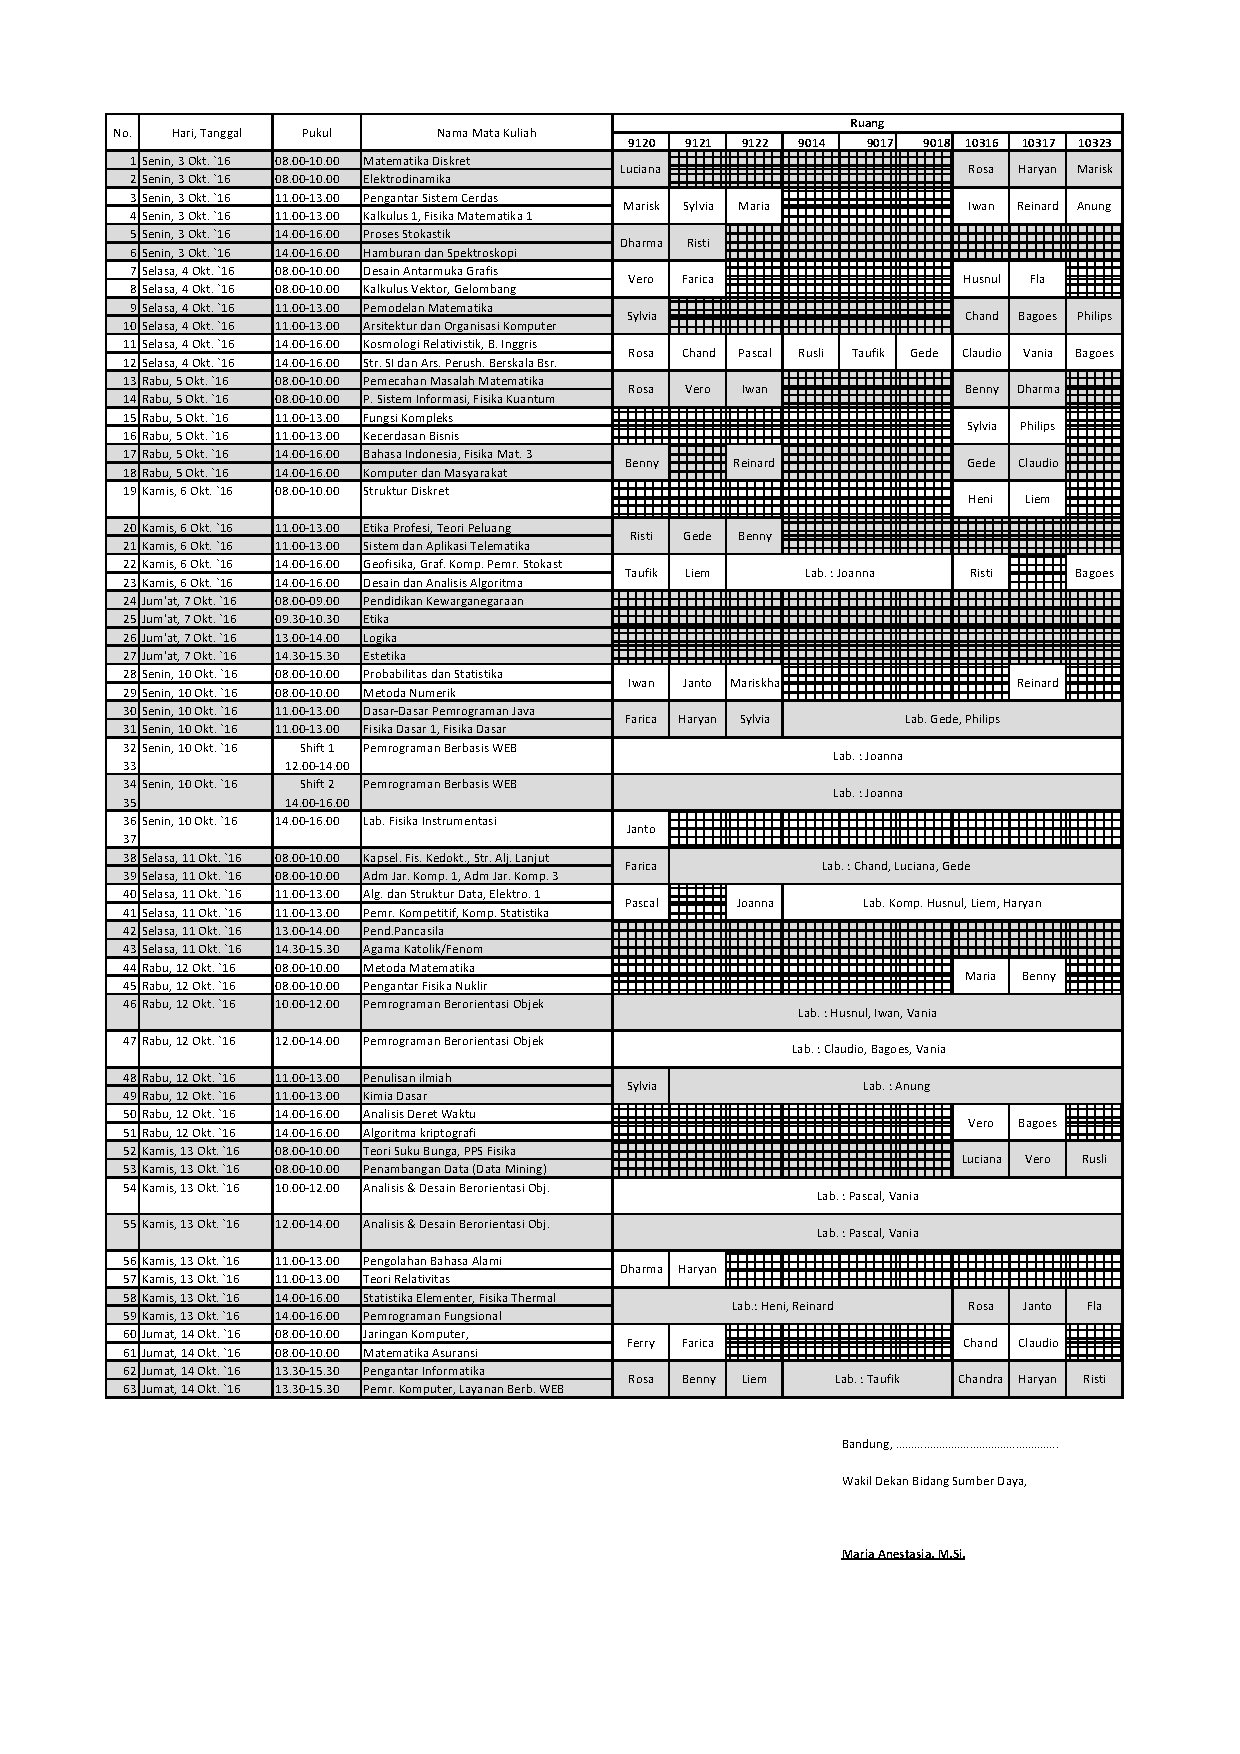
\includegraphics[scale=0.7]{Gambar/JadwalPengawasUTS20161}
		\caption{File Excel Jadwal Mengawas Format Lama}
		\label{fig:formatBaru}
\end{figure}

}{}
\ifdefstring{\vlmpc}{1}{\chapter{The Source Code}
\label{app:C}

%selalu gunakan single spacing untuk source code !!!!!
\singlespacing 
% language: bahasa dari kode program
% terdapat beberapa pilihan : Java, C, C++, PHP, Matlab, R, dll
%
% basicstyle : ukuran font untuk kode program
% terdapat beberapa pilihan : tiny, scriptsize, footnotesize, dll
%
% caption : nama yang akan ditampilkan di dokumen akhir, lihat contoh
\begin{lstlisting}[language=Java,basicstyle=\tiny,caption=MyFurSet.java]

import java.util.ArrayList;
import java.util.Collections;
import java.util.HashSet;

/**
 *
 * @author Lionov
 */

//class for set of vertices close to furthest edge
public class MyFurSet {
    protected int id;                                  //id of the set
    protected MyEdge FurthestEdge;                     //the furthest edge
    protected HashSet<MyVertex> set;                   //set of vertices close to furthest edge
    protected ArrayList<ArrayList<Integer>> ordered;   //list of all vertices in the set for each trajectory
    protected ArrayList<Integer> closeID;              //store the ID of all vertices
    protected ArrayList<Double> closeDist;             //store the distance of all vertices
    protected int totaltrj;                            //total trajectories in the set

    /**
     * Constructor
     * @param id : id of the set
     * @param totaltrj : total number of trajectories in the set
     * @param FurthestEdge : the furthest edge
     */
    public MyFurSet(int id,int totaltrj,MyEdge FurthestEdge) {
        this.id = id;
        this.totaltrj = totaltrj;
        this.FurthestEdge = FurthestEdge;
        set = new HashSet<MyVertex>();
        ordered = new ArrayList<ArrayList<Integer>>();
        for (int i=0;i<totaltrj;i++) ordered.add(new ArrayList<Integer>());
        closeID = new ArrayList<Integer>(totaltrj);
        closeDist = new ArrayList<Double>(totaltrj);
        for (int i = 0;i <totaltrj;i++) {
            closeID.add(-1);
            closeDist.add(Double.MAX_VALUE);
        }
    }

    /**
     * set a vertex into the set
     * @param v : vertex to be added to the set
     */
    public void add(MyVertex v) {
        set.add(v);
    }

    /**
     * check whether vertex v is a member of the set
     * @param v : vertex to be checked
     * @return true if v is a member of the set, false otherwise
     */
    public boolean contains(MyVertex v) {
        return this.set.contains(v);
    }

    /**
     *  create a column for table Gamma, sorted for each row
     */
    public void createColumn() {
        for (MyVertex v : set) {
            for (Integer key : v.vertexnum.keySet()) {
                for (Integer values : v.vertexnum.get(key)) {
                    ordered.get(key).add(values);
                }
            }
        }
        for (ArrayList<Integer> al : ordered) Collections.sort(al);
    }


}
\end{lstlisting}}{}
\ifdefstring{\vlmpd}{1}{\include{Lampiran/lampD}}{}
\ifdefstring{\vlmpe}{1}{\include{Lampiran/lampE}}{}
\ifdefstring{\vlmpf}{1}{\include{Lampiran/lampF}}{}
\ifdefstring{\vlmpg}{1}{\include{Lampiran/lampG}}{}
\ifdefstring{\vlmph}{1}{\include{Lampiran/lampH}}{}
\ifdefstring{\vlmpi}{1}{\include{Lampiran/lampI}}{}

\end{document}
